\documentclass[Master, ngerman, UKenglish, bibstyle=alphabetic]{scrbook}
%------------------------------------------------------------------------------
% This file contains a skeleton thesis for
% a Physics or Astronomy Institute in the University of Bonn.

% Specify the thesis type as an option: PhD, Master, Diplom, Bachelor.
% Specify the thesis stage as an option: Draft (default), Submit, Final, PILibrary.

% Specify the language(s) in the class and then use babel.
% If you need more than one language, give the default language last,
% e.g. ngerman, UKenglish for a thesis in British (UK) English where you want
% to be able to set the language to German for some part of it.

%------------------------------------------------------------------------------
% Pass TeX Live version to the package.
% Use command pdflatex --version to find out which version you are running.
% twoside=true is suitable for printing, while twoside=false is probably better for PDF version.
\usepackage[twoside=true, texlive=2017,subcaption=true]{ubonn-thesis}

%------------------------------------------------------------------------------
% Adjustments to standard biblatex style.
% Change option to backref=false when your thesis is ready to turn off back-referencing.
% Pass the option showurl=false to shorten your bibliography by not including url fields.
\usepackage[backref=true]{ubonn-biblatex}

%------------------------------------------------------------------------------
% Glossary package
% \usepackage[acronym,toc,nosuper]{glossaries}
% TikZ packages and libraries
% \usepackage{tikz}
% \usepackage{tikz-3dplot}
% \usepackage{pgfplots}
% \usetikzlibrary{positioning,shapes,arrows}
% \usetikzlibrary{decorations.pathmorphing}
% \usetikzlibrary{decorations.markings}
\usepackage{thesis_defs}

%------------------------------------------------------------------------------
% Instead of colouring  links, cites, table of contents etc.
% put them in a coloured box for the screen version.
% This is probably a good idea when you print your thesis.
\hypersetup{colorlinks=false,
   linkbordercolor=blue,citebordercolor=magenta,urlbordercolor=darkgreen
 }

%------------------------------------------------------------------------------
% When writing your thesis it is often helpful to have the date and
% time in the output file. Comment this out for the final version.
\ifoot[\today{} \thistime]{\today{} \thistime}

% In order to check if your labels are referenced try the refcheck package
% \usepackage{refcheck}

%------------------------------------------------------------------------------
% biblatex is included by ubonn-thesis. Look there for the settings used.
% See the options for settings that can be changed easily.
% For further changes copy the \RequirePackage[...]{biblatex} here
% and include ubonn-thesis with the option biblatex=false.

% Specify the bibliography files here and not at the end!
% Use standard_refs-bibtex if you use bibtex or bibtex8
% and standard_refs-biber  if you use biber
%\addbibresource{bib/thesis_refs.bib}
\addbibresource{bib/standard_refs-biber.bib}

%------------------------------------------------------------------------------
% The following definitions are used to produce the title pages
% needed at various stages
\newcommand{\thesistitle}{Determination of the beam asymmetry $\Sigma$ in $\eta$- and $\eta'$-photoproduction using Bayesian statistics}
\newcommand*{\thesisauthor}{\textsc{Jakob Michael Krause}}
\newcommand*{\thesistown}{Vechta}
\renewcommand*{\InstituteName}{\HISKP}
\renewcommand*{\inInstitute}{\inHISKP}
\renewcommand*{\InstituteAddress}{\HISKPaddress}
% Adjust \thesisreferee...text depending on male/female referee
\newcommand*{\thesisrefereeonetext}{1.\ Gutachterin}
\newcommand*{\thesisrefereeone}{\textsc{Jun. Prof.\ Dr.\ Annika Thiel}}
\newcommand*{\thesisrefereetwotext}{2.\ Gutachter}
\newcommand*{\thesisrefereetwo}{\textsc{Prof.\ Dr.\ Jochen Dingfelder}}
% Date when thesis was submitted (Master/Diplom)
% Year or Month, Year when thesis was submitted (PhD)
\newcommand*{\thesissubmit}{19.09.2022}
% \newcommand*{\thesissubmit}{Month 2021}
% Date of thesis examination (PhD)
\newcommand*{\thesispromotion}{XX.YY.2021}
% Month and year of the final printed version of the thesis
\newcommand*{\thesismonth}{Sep}
\newcommand*{\thesisyear}{2022}
\newcommand*{\thesisnumber}{BONN-IR-2021-XXX}
% Dedication
% \newcommand*{\thesisdedication}{}

%------------------------------------------------------------------------------
% The abstract is only needed for the printed version and should be in
% English regardless of the language of the thesis
\newcommand{\thesisabstract}{%
  \begin{otherlanguage}{UKenglish}
    This is your thesis abstract. It may be in a language that is
    different from the rest of your thesis.
  \end{otherlanguage}
}

%------------------------------------------------------------------------------
% \includeonly can be used to select which chapters you want to process
% A simple \include command just inserts a \clearpage before and after the file
% Note that \includeonly can be quite picky! Do not forget to put a
% comma after the filename, otherwise it will simply be ignored!
\includeonly{%
   %thesis_intro,
   %thesis_appendix,
   %thesis_acknowledge,
   %experiment,
   event_selection,
   %sigma_eta,
   %sigma_etap,
   %conclusion
 }

%------------------------------------------------------------------------------
% Give a list of directories where figures can be found. Do not leave
% any spaces in the list and end the directory name with a /
\graphicspath{%
  {figs/}%
  {figs/cover/}%
}

%------------------------------------------------------------------------------
% Make a glossary and a list of acronyms
% \makeglossaries

% Glossary entries
% \input{thesis_glossary}

% Draft version - add the word DRAFT on the cover pages
\ifthenelse{\equal{\ThesisVersion}{Draft}}{%
  \usepackage{background}
  \backgroundsetup{contents=DRAFT, color=blue!30}
}

%------------------------------------------------------------------------------
\begin{document}

% Make cover and title pages
\makethesistitle

\pagestyle{scrplain}

%------------------------------------------------------------------------------
% You can add your acknowledgements here - don't forget to also add
% them to \includeonly above
%------------------------------------------------------------------------------
\chapter*{Acknowledgements}
\label{sec:ack}
%------------------------------------------------------------------------------

I would like to thank ...

You should probably use \texttt{\textbackslash chapter*} for
acknowledgements at the beginning of a thesis and
\texttt{\textbackslash chapter} for the end.

%%% Local Variables: 
%%% mode: latex
%%% TeX-master: "../mythesis"
%%% End: 


\tableofcontents

\mainmatter
\pagestyle{scrheadings}

% Turn off DRAFT for the following pages
\ifthenelse{\equal{\ThesisVersion}{Draft}}{%
  \backgroundsetup{contents={}}
}{}

%------------------------------------------------------------------------------
% Add your chapters here - don't forget to also add them to \includeonly above
% !TEX root = master_thesis.tex

%==============================================================================
\chapter{Introduction}
\label{sec:intro}
%This chapter will give a brief introduction into the theoretical concepts that motivate this work. First the Standard Model of Particle Physics is sketched along with characteristics of the strong interaction. Next, the photoproduction of mesons and the importance of polarization observables is explained. Lastly the particular motivation and structure of this work will be presented.
%==============================================================================
%\section{The Standard Model of Particle Physics}
The \emph{Standard Model of Particle Physics} (SM) is the most successful model aiming to describe the particles and forces of the universe. It distinguishes between \emph{fermions} and \emph{bosons}. While all matter consists of fermions, bosons are particles that mediate the fundamental interactions.

Matter consists of (anti-)quarks and (anti-)leptons with three generations of each. Table \ref{tab:sm0} shows all elementary fermions including some of their most important properties. Only the first and lightest generation consists of stable particles, i.e. the up and down quark as well as the electron and its neutrino. All other particles are heavier and not stable, they will thus decay fast via the strong, electromagnetic or weak interaction.

There are in fact four interactions described by the SM: strong, electromagnetic, weak and gravitational interaction \footnote{they are ordered here according to their relative strength}, where gravitation is mentioned here for the sake of completeness; on the mass scale of elementary particles gravitation is negligible. Strong and weak interaction are restricted to a finite range of the order of the nucleon radius, whereas electromagnetic interaction and gravitation have infinite range. Each interaction has its own coupling (charge). The strong interaction is mediated by gluons and couples to the color charge.% A summary of the SM interactions can be found in table \ref{tab:sm1}.
\begin{table}[htbp]
	\centering
	\begin{tabular}{cccccc}
		\toprule
		&\multicolumn{3}{c}{Generation}&el. charge&color charge\\
		&1 & 2 & 3 & & \\
		\hline
		Quarks & $u$&$c$&$t$& 2/3 & r,g,b\\
		&$d$&$s$&$b$& 1/3 & r,g,b\\
		Leptons& $e$&$\mu$&$\tau$&-1& -\\
		& $\nu_e$&$\nu_\mu$&$\nu_\tau$&0&-\\
		\bottomrule

	\end{tabular}
\caption{Summary of the particles of the SM}
\label{tab:sm0}
\end{table}
%\begin{table}[htbp]
%	\centering
%	\begin{tabular}{ccc}
%		\toprule
%		interaction & couples to & Gauge boson\\
%		\hline
%		strong & color & $g$\\
%		elm.& el. charge & $\gamma$\\
%		weak&weak charge & $W^\pm,Z^0$\\
%		\bottomrule
%	\end{tabular}
%
%	\caption{Summary of the interactions of the SM}
%	\label{tab:sm1}
%\end{table}



Gluons and quarks carry color charge and thus interact strongly. However, an isolated quark or gluon has not been observed. Only color neutral bound systems of quarks are seen, which are called hadrons. Hadrons with integer spin are called mesons and those with half-integer spin are called baryons. Color neutrality demands mesons consist of at least one quark and one anti-quark and baryons consist of at least three quarks.


 As already mentioned, isolated quarks are not seen. This can be understood in terms of the strong coupling constant $\alpha_s$. The coupling constant is a measure of the strength of the strong interaction. Because it is highly dependent on the momentum transfer in the observed strong reaction it is also called running coupling constant, which is depicted in figure \ref{fig:coupl}.
 \begin{figure}
 	\centering
 	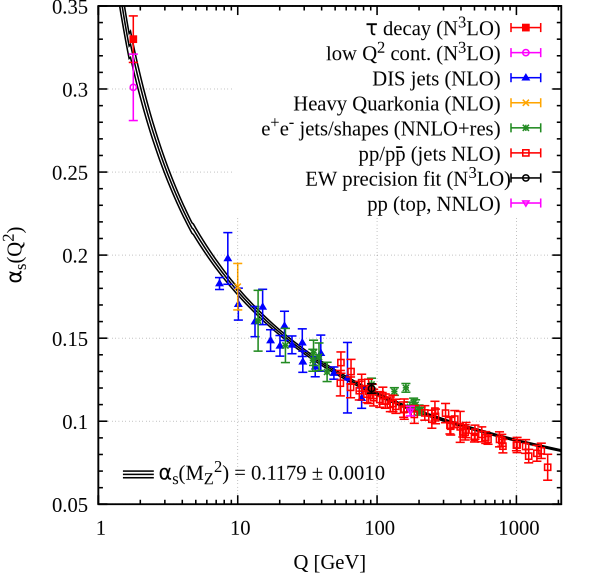
\includegraphics[width=.5\linewidth]{qcd}
 	\caption{Running coupling of QCD. The colored data points represent different methods to obtain a value for $\alpha_s$. For more details it may be referred to \cite{pdg}.}
 	\label{fig:coupl}
 \end{figure}

 For low ($<\SI{1}{\GeV}$) momentum transfers or large distances the coupling constant approaches infinity whereas it decreases for high ($\gg\SI{1}{\GeV}$) momentum transfers or short distances. These momentum ranges are referred to as \emph{confinement} and \emph{asymptotic freedom}, respectively; quarks are confined to remain in a bound state since if one tried to pull them apart the color field becomes so strong it will create a new quark anti-quark pair resulting in two new bound states. On the other hand, bound quarks behave quasi-free and can be described using perturbative quantum chromodynamics (pQCD) if probed at sufficiently large momentum transfers.

 It is more difficult however to describe QCD at momentum scales of $\approx \SI{1}{\GeV}$ since the coupling is too strong to justify a perturbative approach. Thus explicit modeling of QCD bound states is inevitable. One possibility is to describe baryons consisting of constituent quarks which are bound in a potential. Constituent quark models assume baryons are made up of three constituent quarks with effective masses differing from the bare quark mass. The effective mass is made up mostly from a sea of quark anti-quark pairs and gluons which surround the bare (valence) quarks. The explicit form of the binding potential is determined for each model.

 The Bonn model \cite{bonnmodel}, for example, is formulated as a relativistically covariant constituent quark model.
 A potential increasing linearly with the distance is employed to adequately describe confinement. The binding potential between the constituent quarks is described by an instanton-induced interaction. Baryon resonances are then states with an orbital or angular excitation of one of the quarks. Figure \ref{fig:bm} shows computed nucleon, that is Isospin $I=1/2$ resonances, of the Bonn model \cite{bonnmodel} on the left side of each column. These are compared to measured resonances and their PDG rating \cite{pdg} in the middle. Uncertainties are indicated by the colored areas. The resonances are identified by their total angular momentum and their parity $J\pi$. In addition also the total internal angular momentum along with isospin and again the total angular momentum $L_{2T2J}$ is given.
  \begin{figure}[htbp]
 	\centering
 	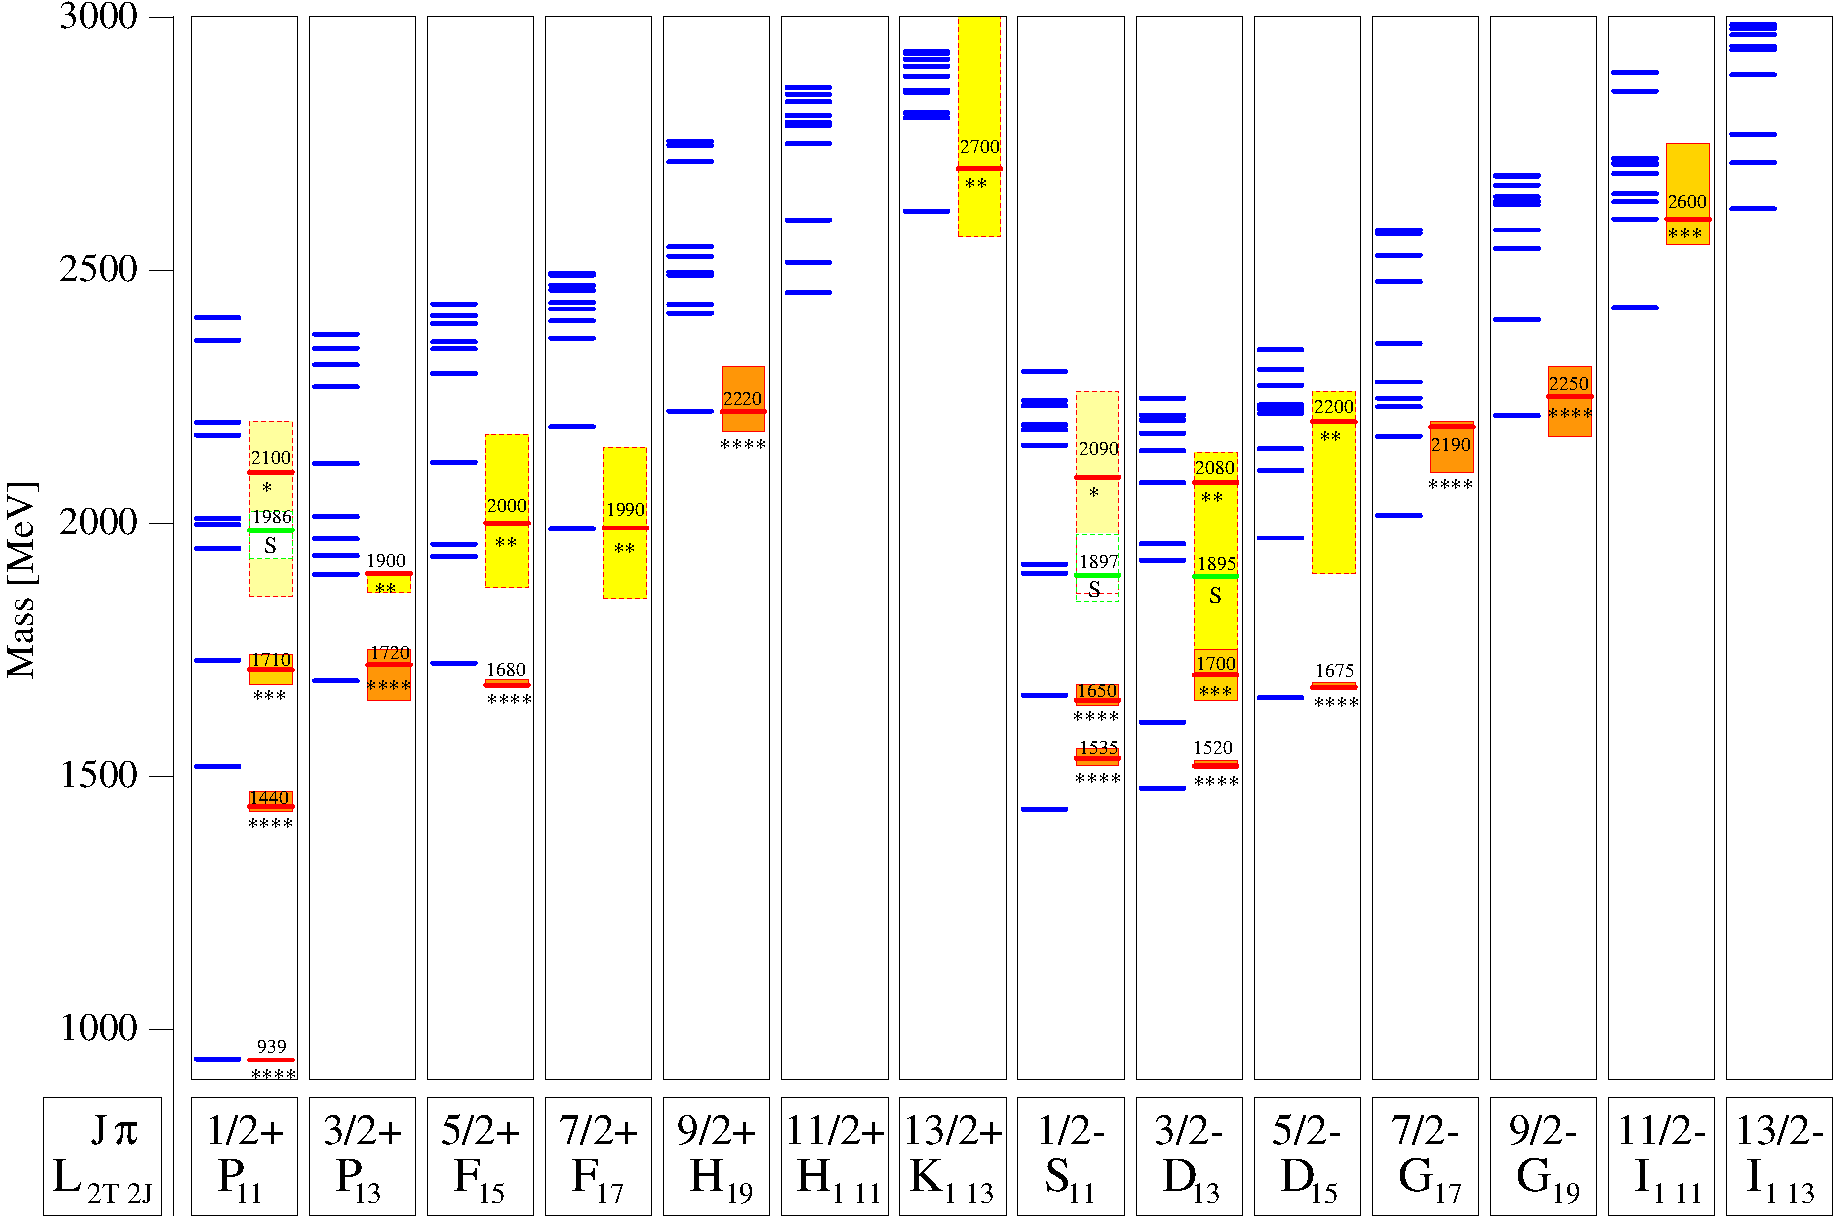
\includegraphics[width=\linewidth]{figs/NucM2.pdf}
 	\caption{Calculated nucleon (isospin $I=1/2$) resonances compared to measurements. Left in each column are the calculations \cite{bonnmodel}, the middle shows the measurements and PDG rating \cite{pdg}}
 	\label{fig:bm}
 \end{figure}
While generally good agreement exists for low lying resonances, especially for high masses there are much more resonances predicted than actually found. This is also known as the problem of the \enquote{missing resonances} indicating the poor understanding of QCD in the non-perturbative region. This can be due to several reasons: most of the knowledge about nucleon resonances and their properties was obtained investigating the $\pi N$ channel, biasing the data for resonances coupling weakly to this channel. Furthermore, the number of excited states with definite quantum numbers is related directly to the effective number of degrees-of-freedom accessible to the underlying theory. As a consequence, the number of degrees-of-freedom should be obtainable by comparing the measured states to the predicted states. Since nucleon resonances decay dominantly hadronic, their resonances are broad and overlapping. Thus on one hand the determination of excitation spectra proves to be a challenge on its own, demanding sophisticated methods, such as partial wave analysis (PWA). On the other hand it is not yet clear how many effective degrees-of-freedom exist for the nucleon in a constituent quark model. They could for example be decreased if the nucleon were made up of a quark and a di-quark structure. In either case it should prove fruitful to investigate the photoproduction of mesons off the nucleon for different final states to access the resonances and transitions between them which are of interest. This should ultimately add to the understanding of QCD in the non-perturbative regime. \cite{Krusche}


\section{Photoproduction of Pseudoscalar Mesons}
From the scattering theory point of view, photoproduction of mesons is well understood \cite{Krusche}. Figure \ref{fig:mes_bildchen} shows schematically the process thereof off the proton:

\begin{figure}[htbp]
	\centering
	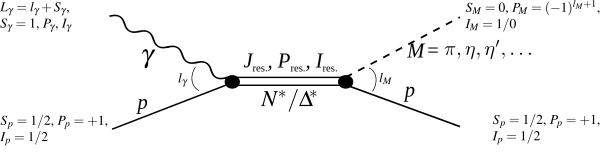
\includegraphics[width=\linewidth]{meson_bildchen}
	\caption{\textsc{Feynman} diagram for the s-channel photoproduction of pseudoscalar mesons, adapted from \cite{farahphd}}
	\label{fig:mes_bildchen}
\end{figure}

The analysis requires partial wave decomposition in both initial and final states \cite{Drechsel} since the intermediate resonance has definite angular momentum, parity  and isospin $J_\text{res.}, P_\text{res.}, I_\text{res.}$. The resonance is excited by a photon with (iso-) spin $I_\gamma,S_\gamma =1$ and parity $P_\gamma$ coupling electromagnetically to the target proton with (iso-) spin $I_p=1/2,S_p=1/2$ and parity $P_p$. The relative momentum is $l_\gamma$, such that the total momentum of the photon is $L_\gamma=l_\gamma+S_\gamma$. Subsequently the intermediate state will have the quantum numbers $J_\text{res.}, P_\text{res.}, I_\text{res.}$ and decay into a pseudoscalar ($S_M=0$) meson with isospin $I_M$, relative orbital angular momentum $l_M$ und Parity $P_M=(-1)^{l_M+1}$ and a proton. The following selection rules can be derived using parity and momentum conservation \cite{Krusche,farahphd}
\begin{align}
	%\left|L_\gamma-S_p\right|&=\left|L_\gamma-1/2\right|\leq J_\text{res.}\leq\left|L_\gamma+1/2\right|=\left|L_\gamma+S_p\right|,\\
	J_\text{res.}&=L_\gamma\oplus S_p = L_\gamma\oplus 1/2,\\
	P_\text{res.}&=P_p\cdot P_\gamma=P_\gamma,\\
	%\left|l_M-S_p\right|&=\left|l_M-1/2\right|\leq J_\text{res.}\leq\left|l_M+1/2\right|=\left|l_M+S_p\right|,\\
	J_\text{res.}&=l_M\oplus S_p = l_M\oplus 1/2\\
	P_\text{res.}&=P_p\cdot P_M=(-1)^{l_M+1},
\end{align}
where the usual rules for the coupling of angular momenta \cite{theo3} apply. Thus, knowledge of the photoproduction multipoles allows the identification of contributing resonances for particular mesonic final states. Table \ref{tab:qn} shows relevant resonances for the lowest order of photon multipoles ($L_\gamma=1$).

\begin{table}[htbp]
	\begin{tabular}{cccccc}
		\toprule
		E
	\end{tabular}
\caption{Allowed quantum numbers for the intermediate resonance state $N^*/\Delta^*$}
\label{tab:qn}
\end{table}

\section{Measurement of Polarization Observables}

\section{Introduction to \textsc{Bayesian} statistics}

\section{Motivation and Structure of this Thesis}
bla

% !TEX root = master_thesis.tex
\chapter{Experimental Setup}
As motivated in the previous chapter, it is promising to study the photoproduction of pseudoscalar mesons in order to determine a complete set of polarization observables. This requires a polarized photon beam and/or a polarized target. It is convenient to study photoproduction off a fixed target and investigate the resonances that occur in the process. Incidentally, these resonances can only be accessed via their decay products, such that suitable calorimeters are needed. The CBELSA/TAPS experiment is  located in Bonn  at the ELectron Stretcher Accelerator (ELSA), which can be used to generate a high energy photon beam using the \emph{bremsstrahlung} process, meets all above mentioned requirements. This chapter will elaborate on the already mentioned parts of the experiment that was used to collect the data needed for the determination of the target asymmetry in $\eta'$ photoproduction.

\section{Production of (polarized) high energy photon beam}
First of all, a high energy photon beam has to be produced.
\begin{figure}[htbp]
	\centering
	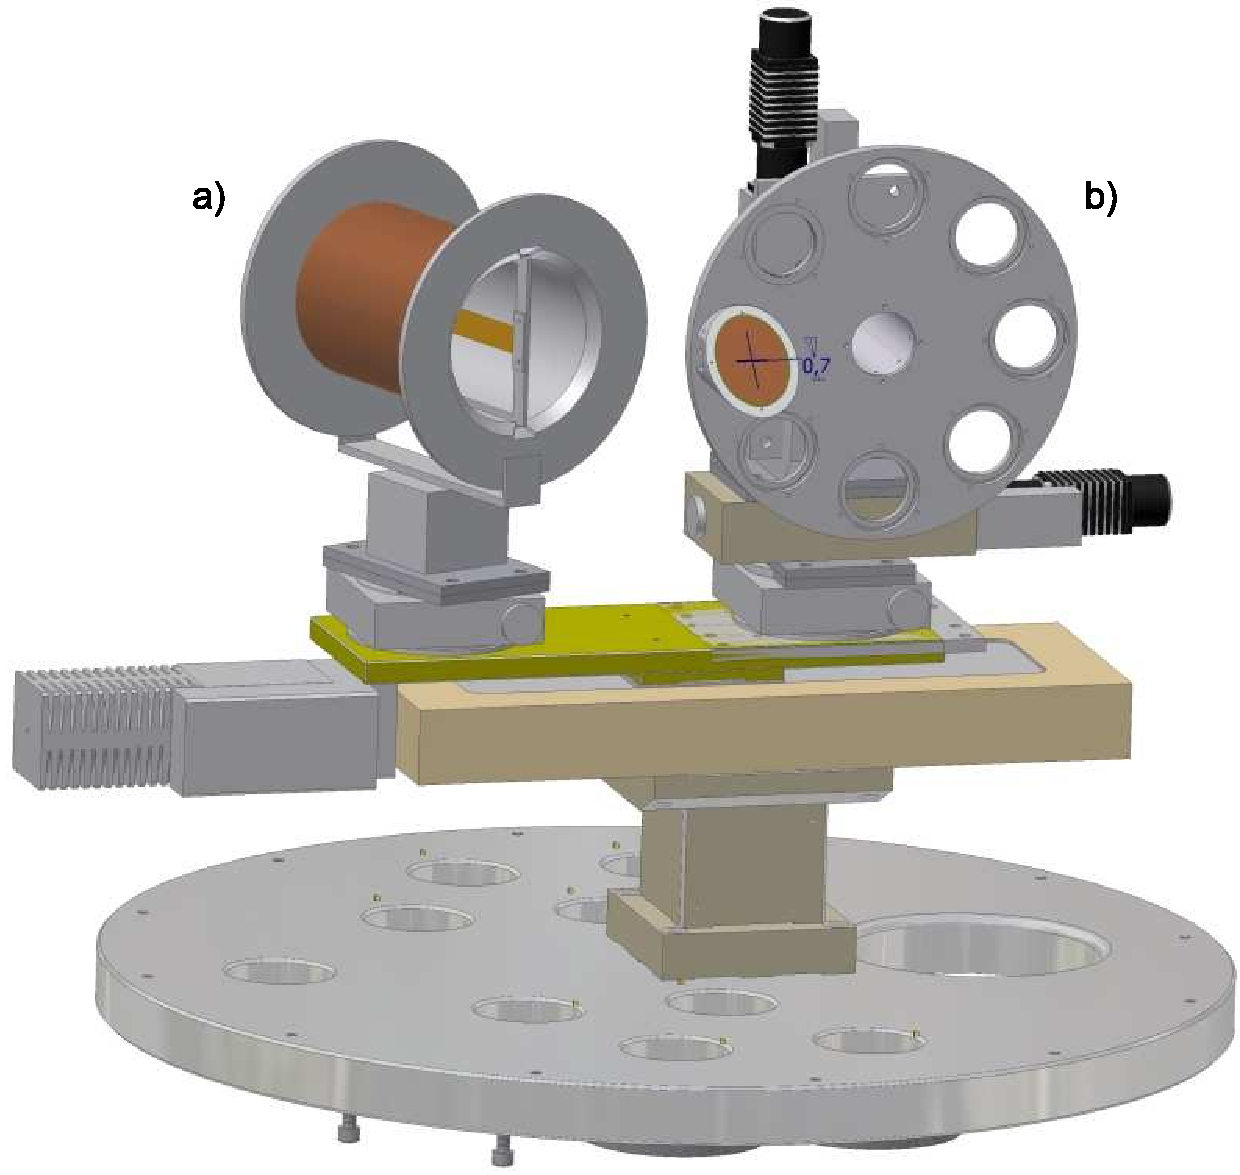
\includegraphics[width=.49\linewidth]{figs/goni-ganz.pdf}
	\caption{\cite{cb}}
\end{figure}
\begin{figure}[htbp]
	\centering
	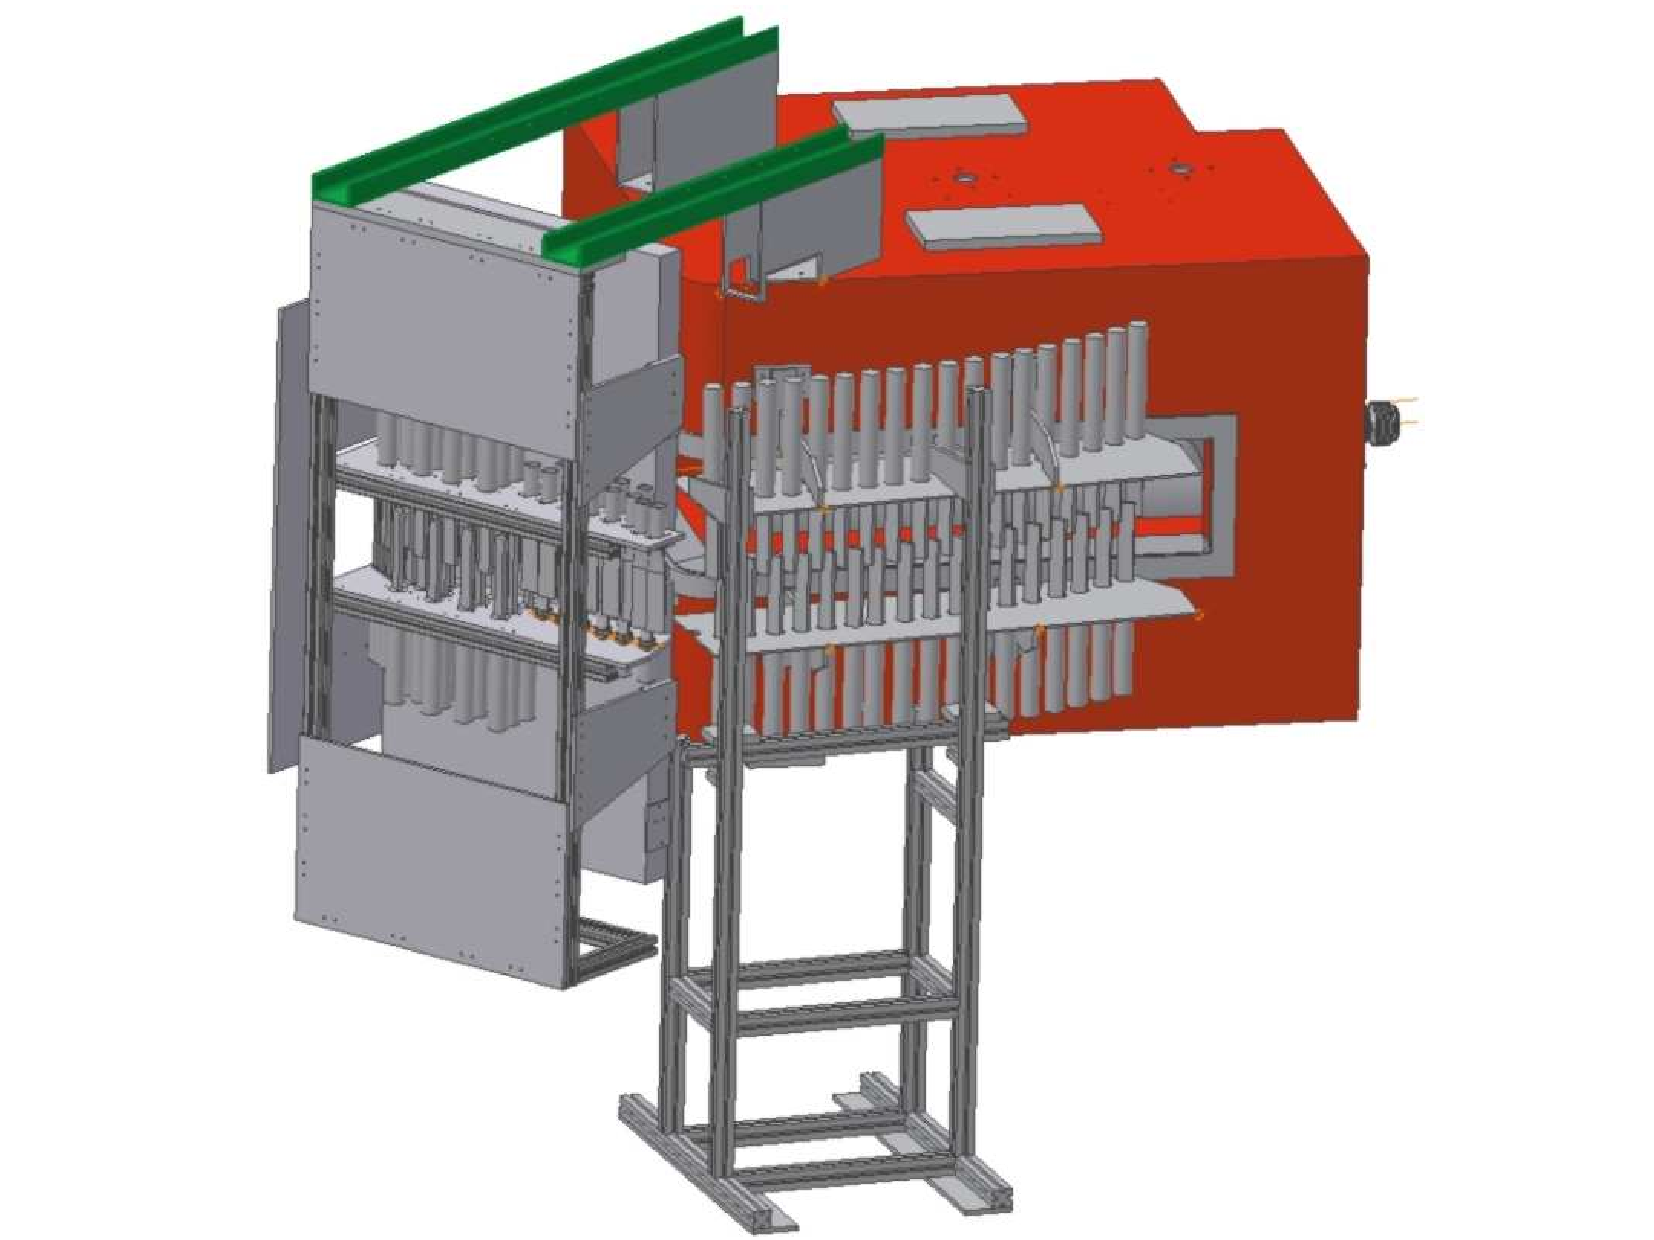
\includegraphics[width=.49\linewidth]{figs/Tagger.pdf}
	\caption{\cite{cb}}
\end{figure}
\subsection{Tagger}
\label{subsec:tag}
\section{Beam Target}

\begin{figure}[htbp]
	\centering
	\includegraphics[width=.5\linewidth]{figs/Target.pdf}
	\caption{\cite{cb}}
\end{figure}
\section{Calorimeters}
\begin{figure}[htbp]
	\centering
	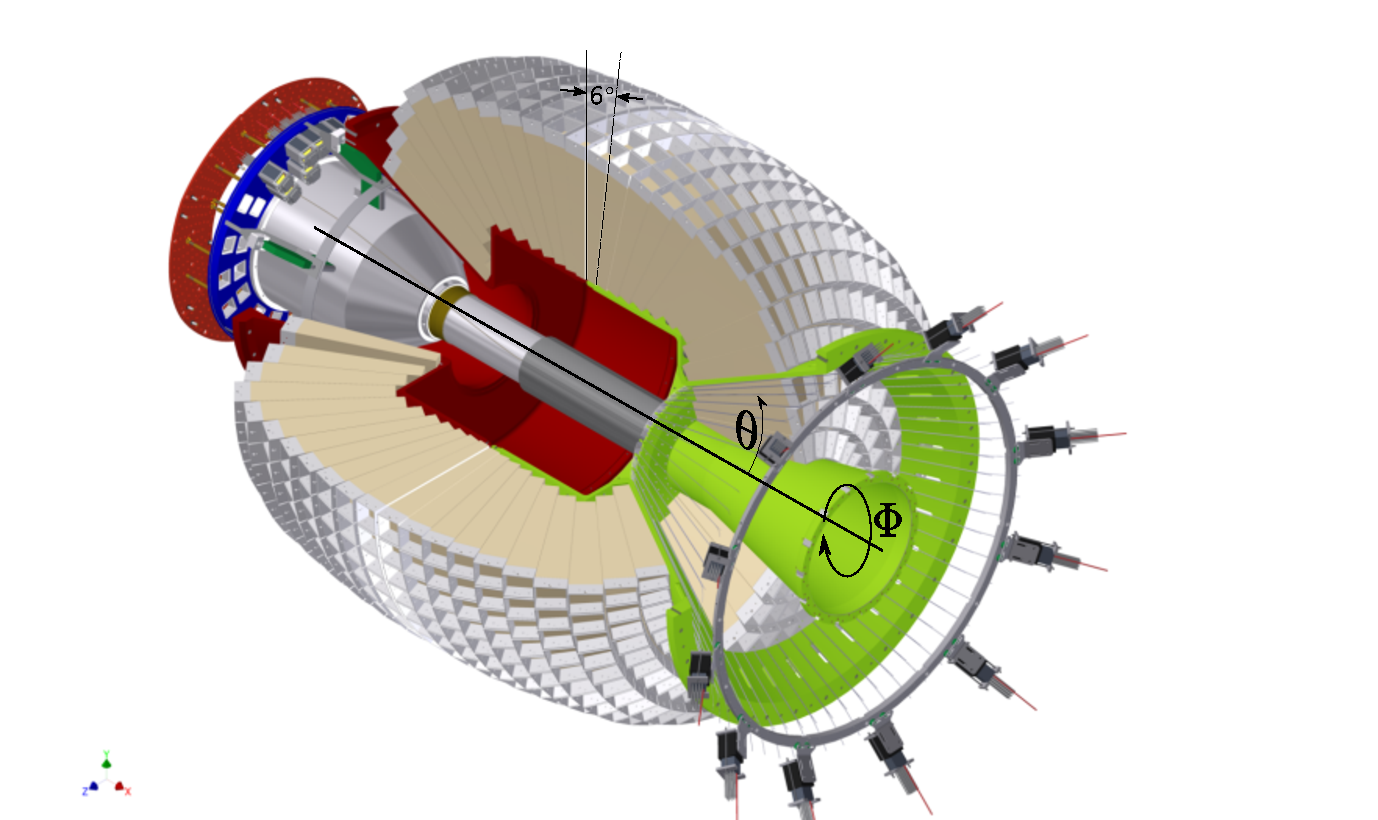
\includegraphics[width=\linewidth]{figs/cb_fp_in.pdf}
	\caption{\textsc{D. Walther} in \cite{urban}}
\end{figure}
\begin{figure}[htbp]
	\centering
	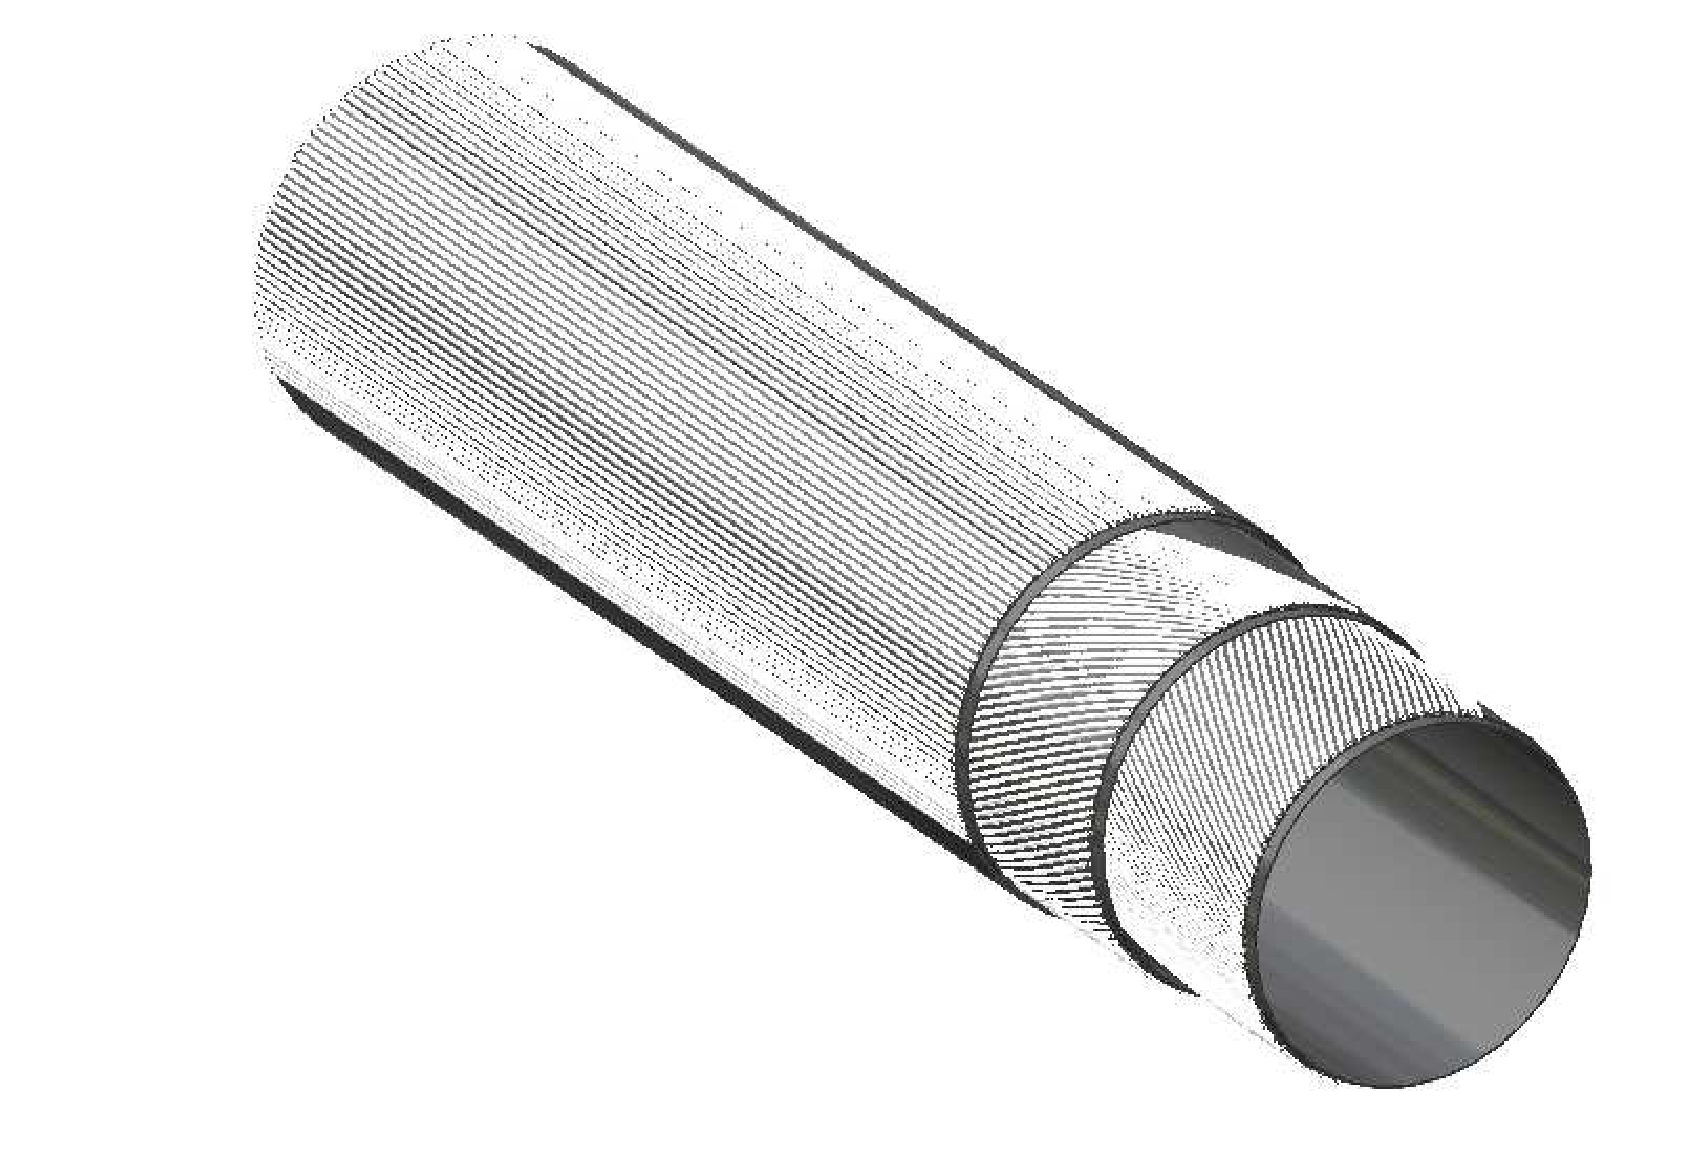
\includegraphics[width=.5\linewidth]{figs/faserorient.pdf}
	\caption{\cite{cb}}
\end{figure}
\begin{figure}[htbp]
	\centering
	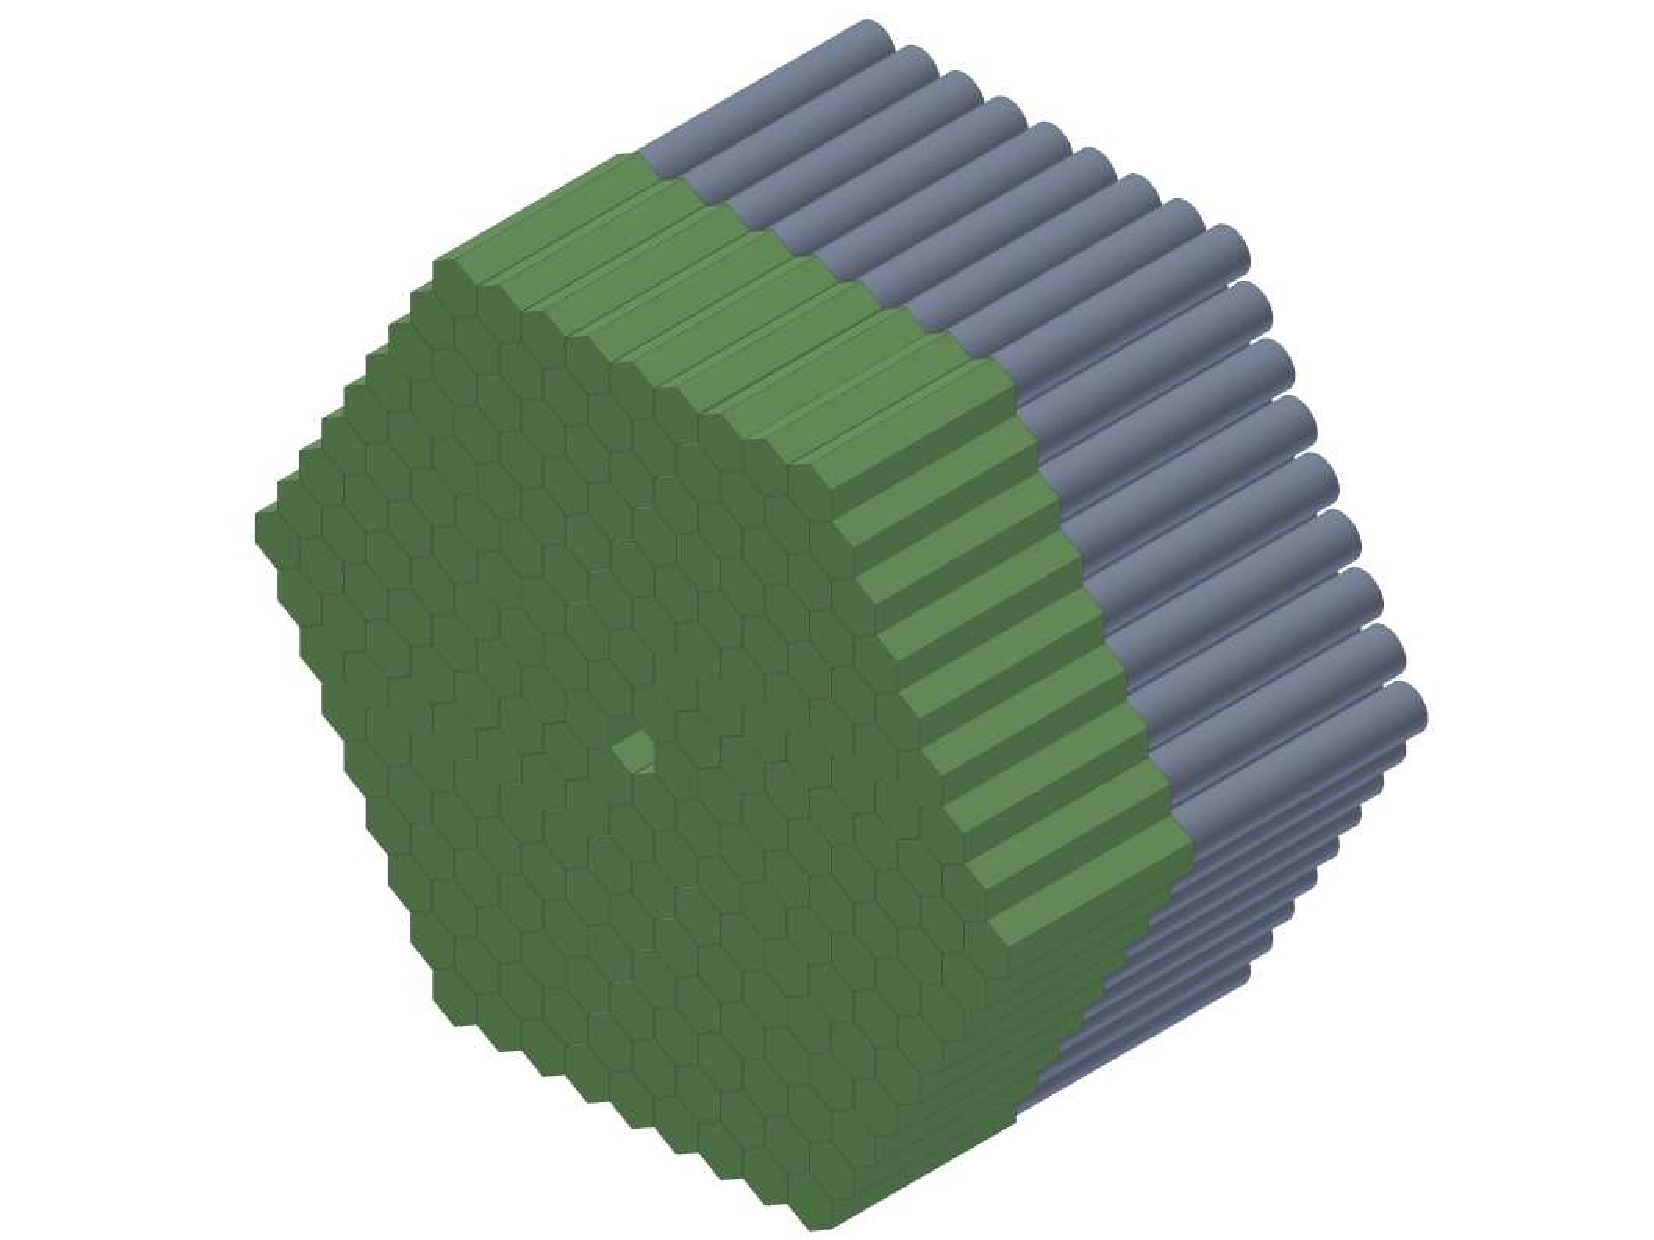
\includegraphics[width=.5\linewidth]{figs/mini-taps.pdf}
	\caption{\cite{cb}}
\end{figure}

\section{Trigger}
% !TEX root = master_thesis.tex
\chapter{Event selection}
The determination of polarization observables needs to be completed for particular reactions (cf. chapter \ref{chap:intro}), such as the photoproduction of e.g. a single $\eta'$ meson. However, the recorded events  contain data from the decay products of all possible final states in addition to combinatorical background. Thus, event candidates for the desired reaction have to be extracted before they are considered for further analysis. Table \ref{tab:etap} shows the five most probable decay modes of the $\eta'$ meson. Three of these result in final states which only contain photons and are thus reliably measurable with the CBELSA/TAPS experiment. Only the $\eta'\to\gamma\gamma$ decay channel was considered for further analysis; the $\omega\gamma$ channel provides negligible statistics and considering the acceptance of detecting six photons in the final state, the expected yield of the $\eta'\to\gamma\gamma$ decays should be roughly equal to the $\eta'\to\pi^0\pi^0\eta\to6\gamma$ final state \cite{farah}. Offering a cleaner, three-particle final state, the $\eta'\to\gamma\gamma$ channel was then favored in the course of this thesis.    
\begin{table}[htbp]
	\centering
	\begin{tabular}{cccc}
		\toprule
		\multicolumn{3}{c}{Decay mode}&Branching ratio\\
		\hline
		$\pi^+\pi^-\eta$&&&42.6\%\\
		$\rho^0\gamma$&$\to$&$\pi^+\pi^-\gamma$ &28.9\% (28.9\%)\\
	$\pi^0\pi^0\eta$&$\to$&$6\gamma$ & 22.8\% (8.8\%)\\
		$\omega\gamma$ &$\to$&$ \pi^+\pi^-\pi^0\gamma/\pi^0\gamma\gamma$&2.52\% (2.2\%/0.21\%)\\
	$\gamma\gamma$&&&2.3\%\\

		\bottomrule
	\end{tabular}
\caption{The five most probable decay modes of the $\eta'$ meson. The most probable further decay with according branching ratio is shown in brackets.\cite{pdg}}
\label{tab:etap}
\end{table}

\noindent The process of \emph{event selection} for the reaction $\gamma p \to p\eta'\to p\gamma\gamma$ is outlined in the following chapter. Note that in this thesis the analysis of data from $\eta$-photoproduction starts with this process already completed, which is described in detail in reference \cite{farahphd}.

\section{Preselection and charge cut}
Since the polarization degree can only be evaluated reliably up to \SI{1800}{\mega\eV} and the production threshold for $\eta'$ mesons is $E_\gamma=\SI{1447}{\mega\eV}$ \cite{pdg}, the beam photon energy range was restricted to \SIrange{1400}{1800}{\mega\eV} from the very beginning. The measured events are then generally classified depending on the number of particle energy deposits (PED). If the complete four-momenta of three final state particles are measured, they are referred to as 3PED events. Low energy protons however may either be only detected in the scintillators of the inner, forward or MiniTAPS detector -- giving only directional information (2.5 PED) -- or lost entirely (2 PED). Only 2.5PED and 3PED events were analyzed since the additional background contributions from 2PED events exceeded the additional signal contributions. It is worth noting that 3PED events are significantly dominant for $\eta'\to\gamma\gamma$ reactions; the production threshold for $\eta'$ mesons is so high energetic that the recoil proton will likely be detected. Figure \ref{fig:PEDs} shows the distribution of the different event classes for $\eta'\to\gamma\gamma$ production in \textsc{Monte Carlo} data, with a clear preference towards 3PED events.

\begin{figure}[htbp]
	\centering
	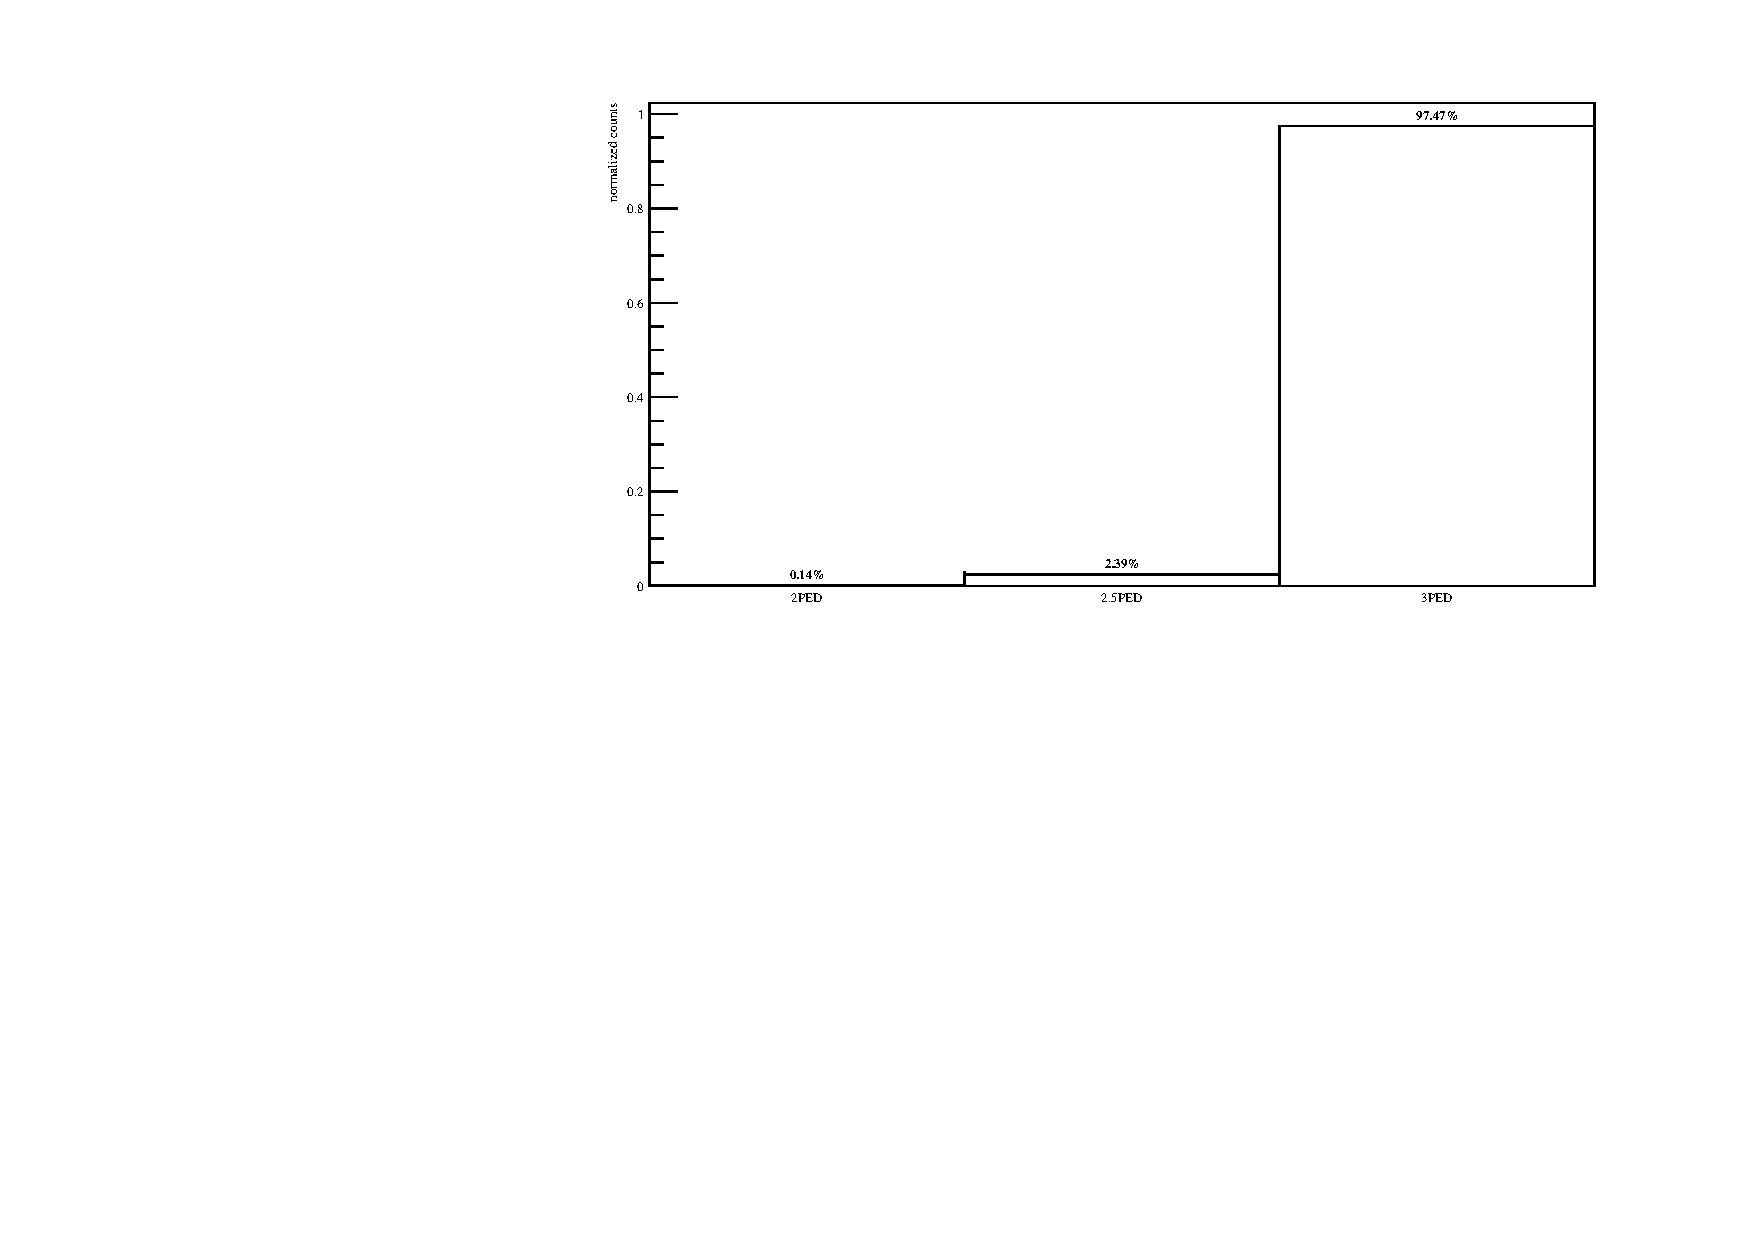
\includegraphics[width=\linewidth]{../figs/hydrogen/PEDs.pdf}
	\caption{Distribution of event classes in $\eta'\to\gamma\gamma$ production}
	\label{fig:PEDs}
\end{figure}
To further improve the signal to background ratio, the charge information of the final state particles was utilized in the next step. In particular, to select  $\eta'\to\gamma\gamma$ reactions, one charged and two uncharged particles in the final state were demanded. 

\section{Time of particles}
\label{sec:time}
Due to its high count rate the tagging system (see section \ref{subsec:tag}) will not only record beam photons which produce the detectable final state particles, but also several uncorrelated ones. To select only beam photons which will induce a photoproduction process the time information of the detected particles is used. It is shown in figure \ref{fig:time} for all particles involved in 2.5PED and 3PED events of $\eta'$ photoproduction. 
\begin{figure}[htbp]
	\centering
	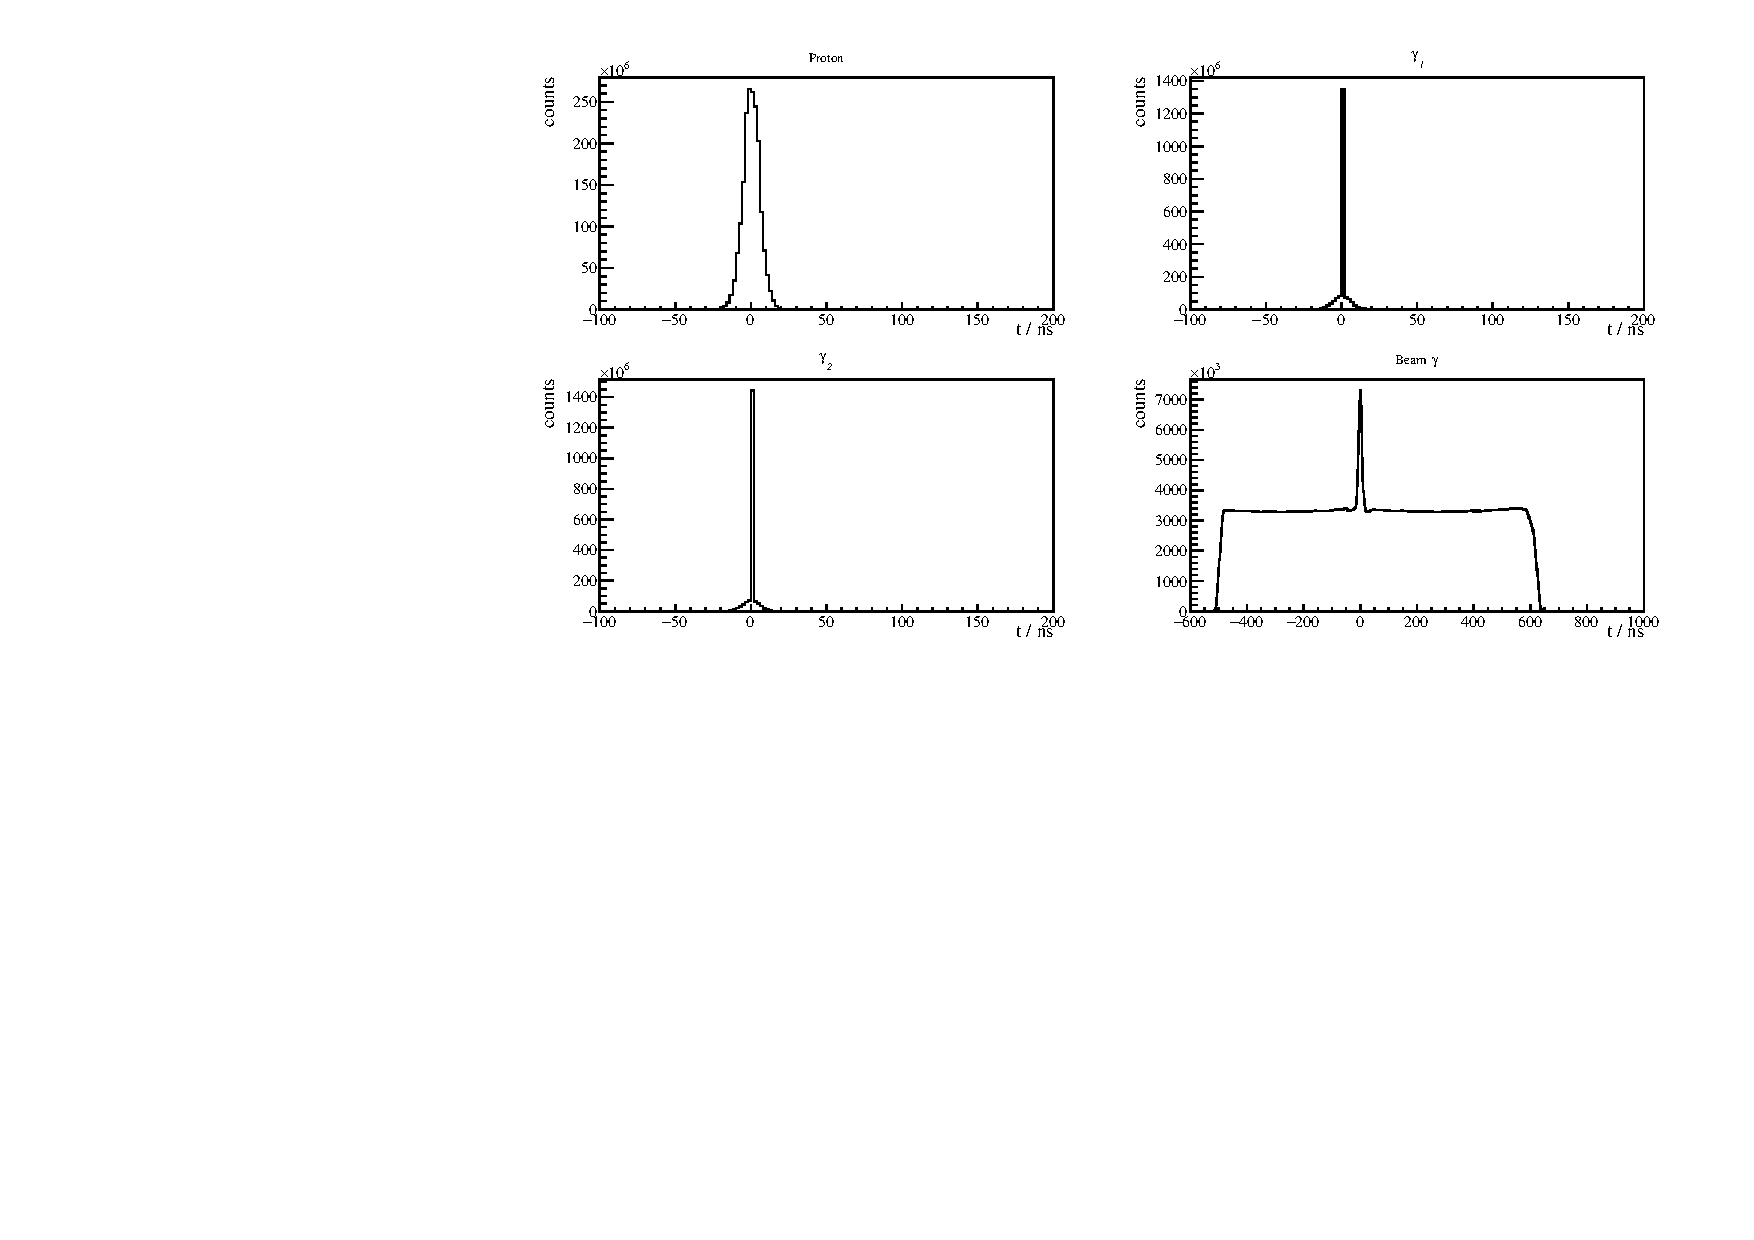
\includegraphics[width=\linewidth]{../figs/hydrogen/time/times.pdf}
	\caption{Time information of all final state particles and the beam photon for 3PED $\eta'$ production}
	\label{fig:time}
\end{figure} 
In all cases prompt peaks centered around \SI{0}{\nano\s} (the trigger time) are visible. Since the final state photons move with velocity $c$ their timing information does not underlie fluctuations, as is the case for the final state proton on the contrary. The tagged, uncorrelated beam photons are visible as flat background underneath the prompt peak in the time of the beam photon. Naturally, only coincident events may be referred to  as $\eta'$ candidates for the further analysis and thus only events with time information of at least one final state particle are kept. Photons need to be detected in the MiniTAPS or forward
detector to acquire time information. To determine coincidence it is convenient to define the \emph{reaction time} 
\begin{equation}
	t_\text{reaction}=\begin{cases}
		t_\text{beam}-t_\text{meson} & \text{ meson time exists}\\
		t_\text{beam}-t_\text{recoil} & \text{ meson time does not exist},
	\end{cases}
\end{equation}
where the meson time $t_\text{meson}$ is appointed either the averaged time of both decay photons or the time of a single photon if only one photon has time information. $t_\text{beam}$ and $t_\text{recoil}$ are the time of the beam photon and recoil proton, respectively. Figure \ref{fig:time_r} shows the reaction time for 2.5PED and 3PED events; a clear prompt peak centred at 0 is visible, the colored area indicates the chosen range of $t_\text{reaction}\in[-8,5]\si{\nano\s}$. However, this cut still contains random time background underneath the prompt peak. This may be accounted for by \emph{sideband substraction}, assuming the background is flat. All events residing in the prompt peak with $t_r\in[-8,5]\si{\nano\s}$ will be assigned a weight of $w_p=+1$ while sideband events with $t_r\in[-200,-100]\si{\nano\s}\lor t_r\in[100,200]\si{\nano\s}$ will be assigned a weight of $w_s=-\frac{13}{200}$. Events with $t_r$ neither in the sideband nor in the prompt peak get assigned a weight of $w=0$. Any histogram $N$ that is filled in the following will then consist of prompt peak events $N_\text{prompt}$ and sideband events $N_\text{sideband}$ $$N=N_\text{prompt}+w_s\cdot N_\text{sideband},$$ such that the random time background underneath the prompt peak is substracted. In addition, the time difference between meson and proton and between the two photons is demanded to be within $[-10,10]\si{\nano\s}$. All described cuts to the data, including the sideband substraction are referred to as the \emph{time cut} in the following.

\begin{figure}[htbp]
	\centering
	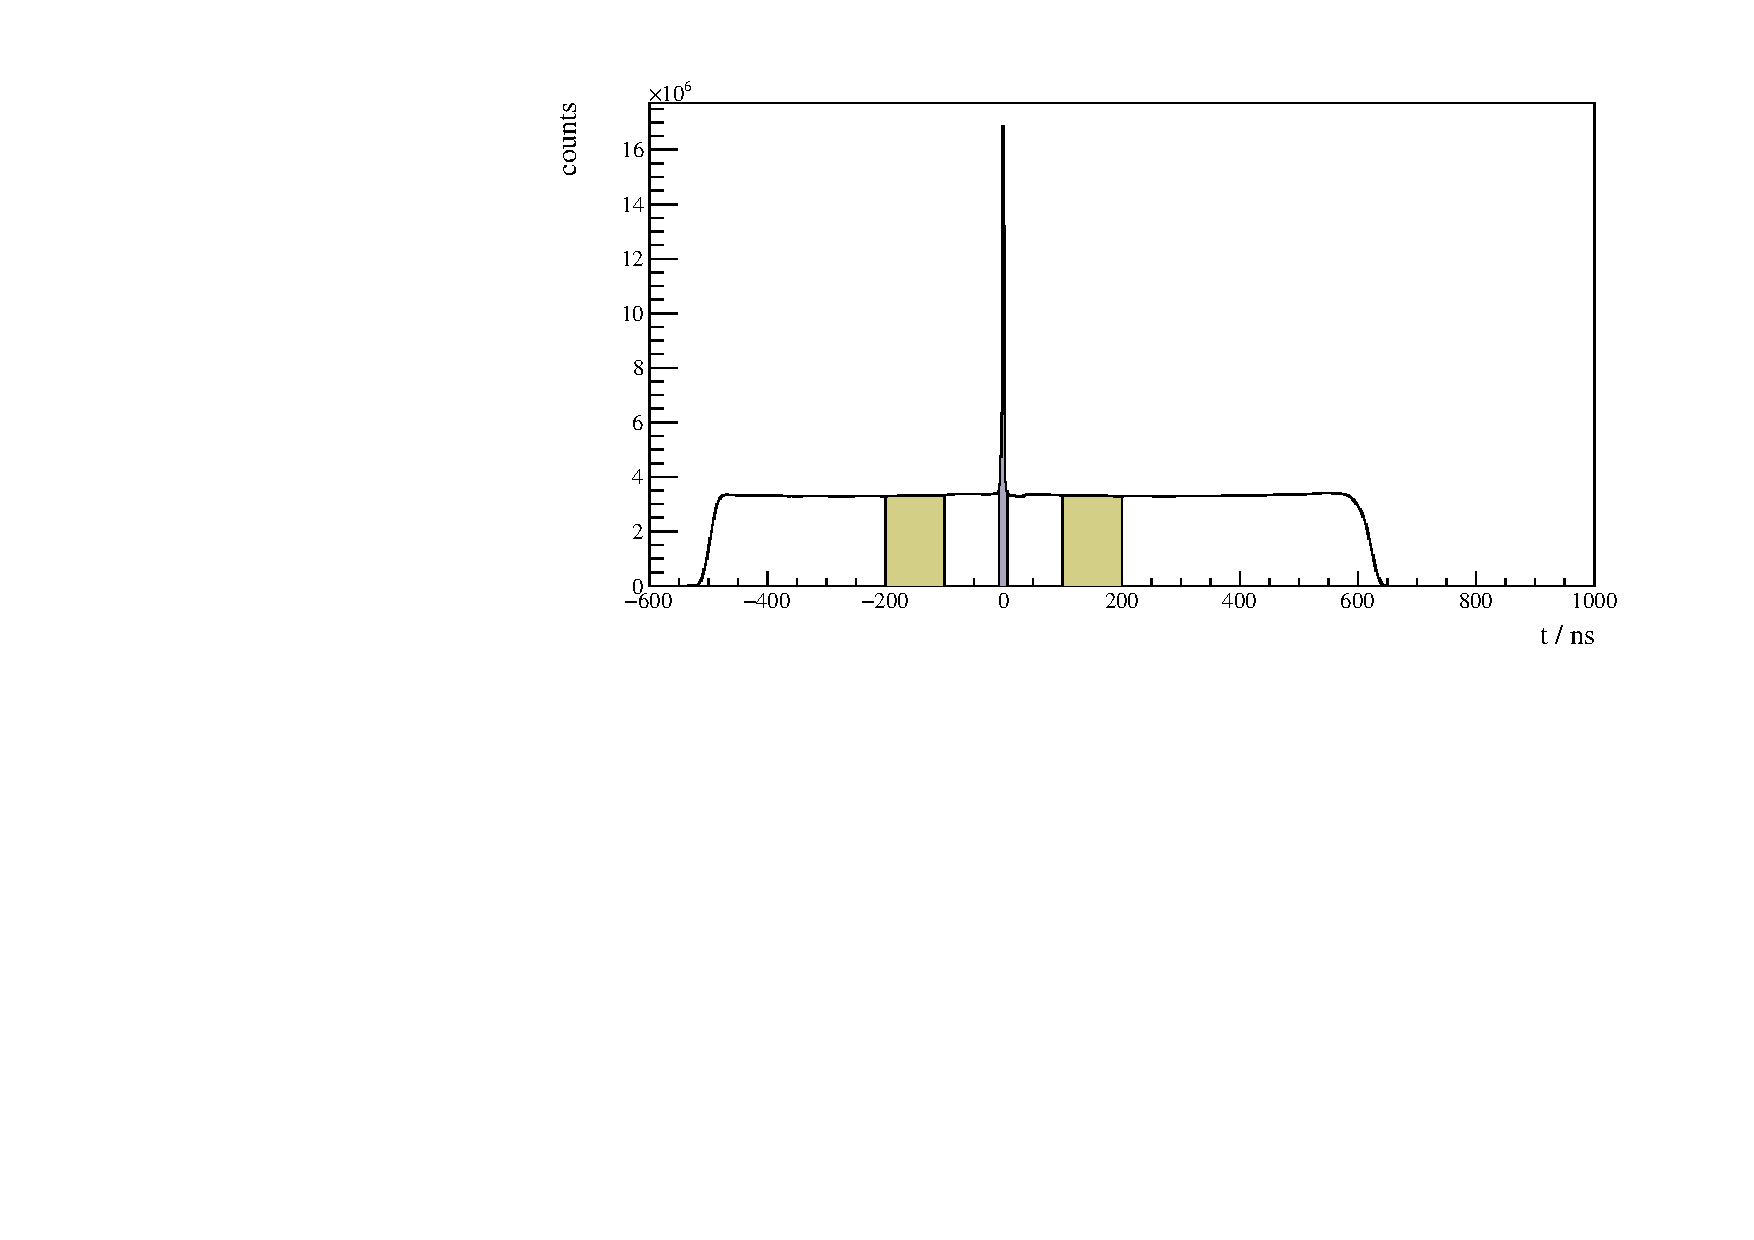
\includegraphics[width=\linewidth]{../figs/hydrogen/time/reaction_time.pdf}
	\caption{Reaction time $t_r$ for 3PED $\eta'$ production}
	\label{fig:time_r}
\end{figure} 

\section{Kinematic constraints}
Up until now mainly combinatorical background was discussed. However one can derive kinematical constraints from energy and momentum conservation to exclusively select the desired reaction. The derivation is discussed first, followed by the determination of the derived cut conditions.
\subsection{Derivation of cut conditions}
Let $p_\text{beam}$ and $p_p$ be the four momenta of the initial state beam photon and proton, respectively. Then \begin{equation}
	p_\text{beam}+p_p=p_\text{recoil}+p_\text{meson}
	\label{eq:kin}
\end{equation}
holds, with $p_\text{recoil}$ being the momentum of the recoiling proton and $p_\text{meson}$ the meson momentum.
\subsubsection{Coplanarity}
In the initial state there is vanishing transversal momentum $p_{xy}$ since the target protons are at rest and the beam photon impinges in $z$-direction. Naturally, this transversal momentum has to vanish in the final state as well, such that \begin{equation}
	\mathcal{P}_{xy} \left[p_\text{recoil}+p_\text{meson}\right]=0,
	\label{eq:copl}
\end{equation}
where $\mathcal{P}_{xy}$ is the projection operator to the transversal plane. Equation \eqref{eq:copl} is valid if and only if meson and proton lie back to back (coplanar) in the $x$-$y$ plane, which is quantified by the difference of their azimuthal angles $\phi_\text{meson}$ and $\phi_\text{recoil}$ being $\SI{180}{\degree}$ in the laboratory-frame
\begin{equation}
	\Delta\phi:=\phi_\text{meson}^\text{LAB}-\phi_\text{recoil}^\text{LAB}\overset{!}{=}\SI{180}{\degree}.
\end{equation}
\subsubsection{Polar angle difference}
If all initial and final state momenta are measured, the reaction described by equation \eqref{eq:kin} is \emph{overdetermined}, such that one final state particle can be treated as a "missing particle" $X$ with momentum $p_X$: 
\begin{equation}
	p_X=p_\text{beam}+p_p-p_\text{meson}.
	\label{eq:polangle}
\end{equation}
One can then use 
\begin{equation}
\Delta\theta:=\theta_{p_X}^\text{LAB}-\theta_{p_\text{recoil}}^\text{LAB}\overset{!}{=}0
\label{eq:polarangle}	
\end{equation}
as a further constraint to the data.
\subsubsection{Missing mass}
The previously described angular cuts are only applicable if all final state particles have been detected. Independently of the detection of the recoil proton the mass of the missing particle $m_X^2=p_X^2$ can be determined and compared with the proton mass of $m_p=\SI{938.27}{\mega\eV}$ \cite{pdg}. From equation \eqref{eq:polangle} it follows that \begin{equation}
	m_X=\sqrt{(E_\gamma+m_p-E_\text{meson})^2-p_{x,\text{meson}}^2-p_{y,\text{meson}}^2-(E_\gamma-p_{z,\text{meson}})^2}.
	\label{eq:mism}
\end{equation}
\subsubsection{Invariant mass}
The measurement of the invariant mass of the two final state photons does also not require the measurement of the recoil proton. The knowledge of both four-momenta suffices, since \begin{equation}
	m_\text{meson}=\sqrt{p_\text{meson}^2}=\sqrt{(p_{\gamma_1}+p_{\gamma_2})^2}=\sqrt{2E_{\gamma_1}E_{\gamma_2}(1-\cos\alpha_{\gamma_1\gamma_2})},
\label{eq:invm}
\end{equation}
where $E_{\gamma_i}$ are the measured photon energies and $\alpha_{\gamma_1\gamma_2}$ is the angle spanned by the two photon momenta. To select only $\eta'$ candidates $m_\text{meson}=m_{\eta'}=\SI{957.78}{\mega\eV}$ is demanded. Remarkably, the cut on the invariant mass of the final state photons is the only one to uniquely select $\eta'$ production candidates so far. All other cuts apply similarly to arbitrary meson photoproduction.
\subsection{Determination of cut ranges}
The constraints described in the previous section must not be understood as strict equalities, cf. equations \eqref{eq:copl},\eqref{eq:polarangle},\eqref{eq:mism} and \eqref{eq:invm}. The quantities of interest will rather describe distributions around the desired value, such that confidence intervals may be extracted by fitting to said distributions. This is done iteratively:

Let $\mathcal{C}^\chi_{\mathcal{I}}$ be the cut operator that restrains the data $\mathcal{D}$ such that the (generic) cut variable $$\chi\in\{\Delta\theta,\Delta\phi,m_X,m_\text{meson}\}$$ lies in the interval $\mathcal{I}\subseteq\mathbb{R}$, such that 
\begin{equation}
	\mathcal{C}_{\mathcal{I}}^\chi:\mathcal{D}\mapsto\mathcal{D}_{\chi\in\mathcal{I}} .
\end{equation}
	 After a first inspection of the data, initial guesses for the intervals $\mathcal{I},\mathcal{J},\mathcal{K},\mathcal{L}$ corresponding to the quantities $\Delta\theta,\Delta\phi,m_X,m_\text{meson}$, respectively, are made.
	Having established estimates for the cut ranges, new ones are estimated by investigating the distribution of one cut variable obtained from the data while all other cut variables are constrained to the previously determined intervals. For example 
	$$\Delta\theta\left(\mathcal{C}_\mathcal{J}^{\Delta\phi}\mathcal{C}_\mathcal{K}^{m_X}\mathcal{C}_\mathcal{L}^{m_\text{meson}}\mathcal{D}\right)\sim \text{normal}(\mu,\sigma),$$
	where $\mu\approx0$. This is done (with some adjustments to the fit function) for each cut variable. The parameters of the gaussian are determined from a $\chi^2$ fit and used to assign new cut ranges. Simultaneously, Monte-Carlo (MC) data of relevant final states are fitted to match the measured values bin-wise. This is done on the one hand to check consistency between measured and MC data and on the other hand used to determine contributing background reactions. First, all mesonic final states that decay into two photons are considered, i.e. $p\pi^0,p\eta,p\eta'$, since the according peaks in the invariant mass spectrum will be visible. Also, a peak at the mass of the $\omega$ (vector)-meson $m_\omega$ will be visible; this stems from photoproduction reactions $p\omega\to p\pi^0\gamma\to p3\gamma$ where one low energetic final state photon is lost, such that the reconstructed invariant mass still estimates the $\omega$ mass. Further, one should investigate the impact of neutral final states, where some of the final state photons may get lost during reconstruction, as can be observed for $p2\pi^0,p\pi^0\eta,p3\pi^0,p2\pi^0\eta$ \footnote{all mesons $m$ decaying into two photons is implied: $m\to\gamma\gamma \forall m$} production. Lastly, possible misidentifiaction of charged particles which then mimic a $p\gamma\gamma$ final state are examined, such as $p\pi^+\pi^-$ and $n\pi^+$. Table \ref{tab:mc} lists all employed MC reactions and their respective final state particles, as well as a short explanation why the particular reaction was included in the fit.
	
	\begin{table}[htbp]
		\begin{tabular}{ccc}
			\toprule
			Photoproduction reaction &Final state particles&Explanation\\
			\hline
			$p\pi^0$ & $p\gamma\gamma$&prominent peak in the invariant mass spectrum \\
			$p\eta$ & $p\gamma\gamma$& \\
			$p\omega$ & $p\pi^0\gamma\to p3\gamma$& \\
			$p\eta'$ & $p\gamma\gamma$&\\
			$p2\pi^0$ & $p4\gamma$&lost photons cause a "3-particle" final state\\
			$p\pi^0\eta$ & $p4\gamma$&\\
			$p3\pi^0$ & $p6\gamma$&\\
			$p2\pi^0\eta$ & $p6\gamma$&\\
			$p\pi^+\pi^-$ &&misidentification of charged particles\\
			$n\pi^+$ &&\\
			\bottomrule
		\end{tabular}
	\caption{Examined MC reactions that were used in sum for the fit}
	\label{tab:mc}
	\end{table}
	
	 Since the invariant mass spectrum features rich contributions from many final states, it is difficult to describe by a (sum of) gaussian function(s), especially considering the background contributions. Thus, for the invariant mass the cut ranges are obtained from gaussian fits to the scaled MC data of the $\eta'$ final state. Table \ref{tab:cuts} shows which fit function and cut range was used for each cut variable. In addition, it shows if the cut ranges were determined from MC or measured data.
	\begin{table}[htbp]
		\centering
		\begin{tabular}{cccc}
			\toprule
			cut variable & fit function & interval range & obtained from\\
			\hline
			$\Delta\theta$&\textsc{Gauss}&$\mathcal{I}'=[\mu-3\sigma,\mu+3\sigma]$&data points\\
			$\Delta\phi$&\textsc{Gauss}&$\mathcal{J}'=[\mu-3\sigma,\mu+3\sigma]$&data points\\
			$m_X$&\textsc{Novosibirsk} \cite{nov}&$\mathcal{K}'=[\mu-2\sigma,\mu+2\sigma]$&data points\\
			$m_\text{meson}$&\textsc{Gauss}&$\mathcal{L}'=[\mu-2\sigma,\mu+2\sigma]$&MC data\\
			
			\bottomrule
		\end{tabular}
		\caption{Fit functions and cut ranges for each variable}
		\label{tab:cuts}
	\end{table}
The newly obtained intervals $\mathcal{I}',\mathcal{J}',\mathcal{K}',\mathcal{L}'$ serve again as input for the previous step. This is repeated until a certain convergence is reached, which is usually the case after a two or three iterations.
 Since the cut ranges may vary depending on beam energy and meson direction, they are determined in bins of the beam energy and the polar angle of the meson in the center of mass system (CMS) $$(E_\gamma,\cos\theta_{\eta'}^\text{CMS}) \footnote{If not otherwise specified, from now on $\cos\theta=\cos\theta_{\eta'}^\text{CMS}$}.$$ Respecting the $\eta'$ final state statistics, a binning of $\Delta E_\gamma=\SI{100}{\mega\eV}$ and $\Delta\cos\theta=1/3$ was chosen, spanning the energy range of \SIrange{1500}{1800}{\mega\eV}. The theoretically accessible lower limit in the beam energy is provided by the production threshold of $\eta' $ mesons at \SI{1447}{\mega\eV} \cite{pdg}. Yet, the binning has to comply with the upper beam energy limit which is bounded from above \footnote{Significantly beyond the coherent edge, the systematic error for the beam polarization  degree gets too large ($>10\%$)} by the position of the coherent edge of the beamtime. It is given by \SI{1700}{\mega\eV} and \SI{1800}{\mega\eV} for the July/August and September/October beam times, respectively. If one were to include the production threshold into the analyzed range using the same binning, more background than $\eta'$ events are collected from \SIrange{1400}{1500}{\mega\eV} (see subsection \ref{subsec:addcuts}), hence the chosen binning starts at \SI{1500}{MeV}.
 
 \subsubsection{Coplanarity}
 Figure \ref{fig:copl} shows the coplanarity spectra for the energy bin $\SI{1500}{\mega\eV}\leq E_\gamma<\SI{1600}{\mega\eV}$ and all angular bins. The data points are visualized by the open circles with error bars, while the black solid histogram is a fit of $\eta'\to\gamma\gamma$ MC. As expected, a clear peak is visible at $\Delta\phi=\SI{180}{\degree}$, which shows only slight dependence on beam energy and meson direction. A $3\sigma$ interval obtained from a gaussian fit is indicated by the dashed red lines. Note that only MC spectra of the $\eta'$ final state were fitted to the data since the coplanarity gives little reference points for a correct estimation of other final states that may contribute. 
   \begin{figure}[htbp]
 	\centering
 	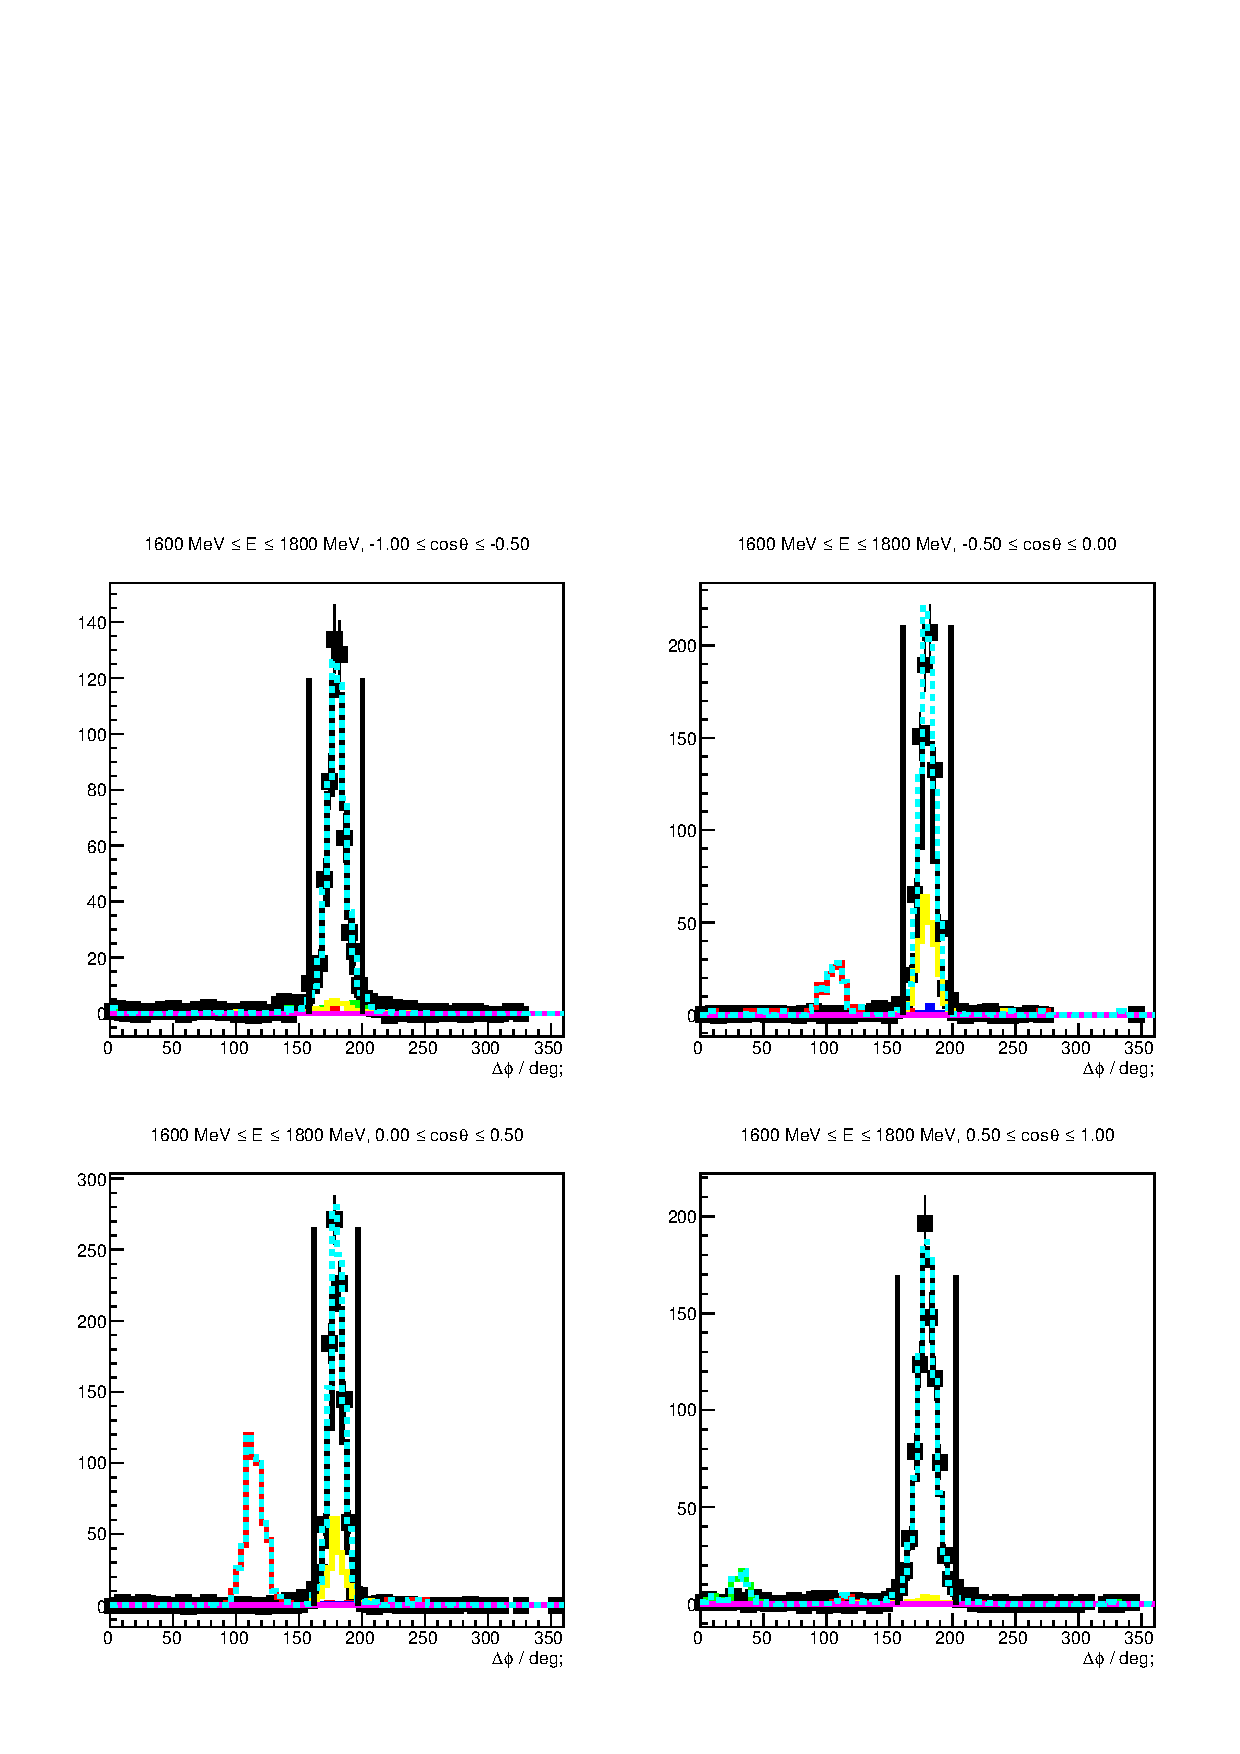
\includegraphics[width=\linewidth]{../figs/hydrogen/bin_cuts/phicut_ebin1.pdf}
 	\caption{Coplanarity of the $p\eta'$ final state with all other cuts applied for the energy bin $\SI{1500}{\mega\eV}\leq E_\gamma<\SI{1600}{\mega\eV}$. The vertical dashed lines show the cut ranges obtained from a gaussian fit to the data (open circles). The solid black histograms represent fitted MC data of $\eta'\to\gamma\gamma$}
 	\label{fig:copl}
 \end{figure}
 \subsubsection{Polar angle difference}
 Since the meson direction correlates with the detector(s) the final state photons hit, the polar angle difference depicts a clear directional dependence as can be seen in figure \ref{fig:pol} for the energy bin $\SI{1500}{\mega\eV}\leq E_\gamma<\SI{1600}{\mega\eV}$ and all angular bins. In the CMS frame, meson and proton are emitted back to back. Thus, if the meson is emitted in backward direction ($\cos\theta\sim -1$), the proton will be detected either in the forward or MiniTAPS detector, which have a better angular resolution than the Crystal Barrel calorimeter, leading to narrower distributions of $\Delta\theta$. The determined cut ranges are $3\sigma$ intervals obtained from a gaussian fit to the data and are indicated by the red dashed lines. As before, no other than $\eta'$ MC are fitted to the spectra.
  \begin{figure}[htbp]
 	\centering
 	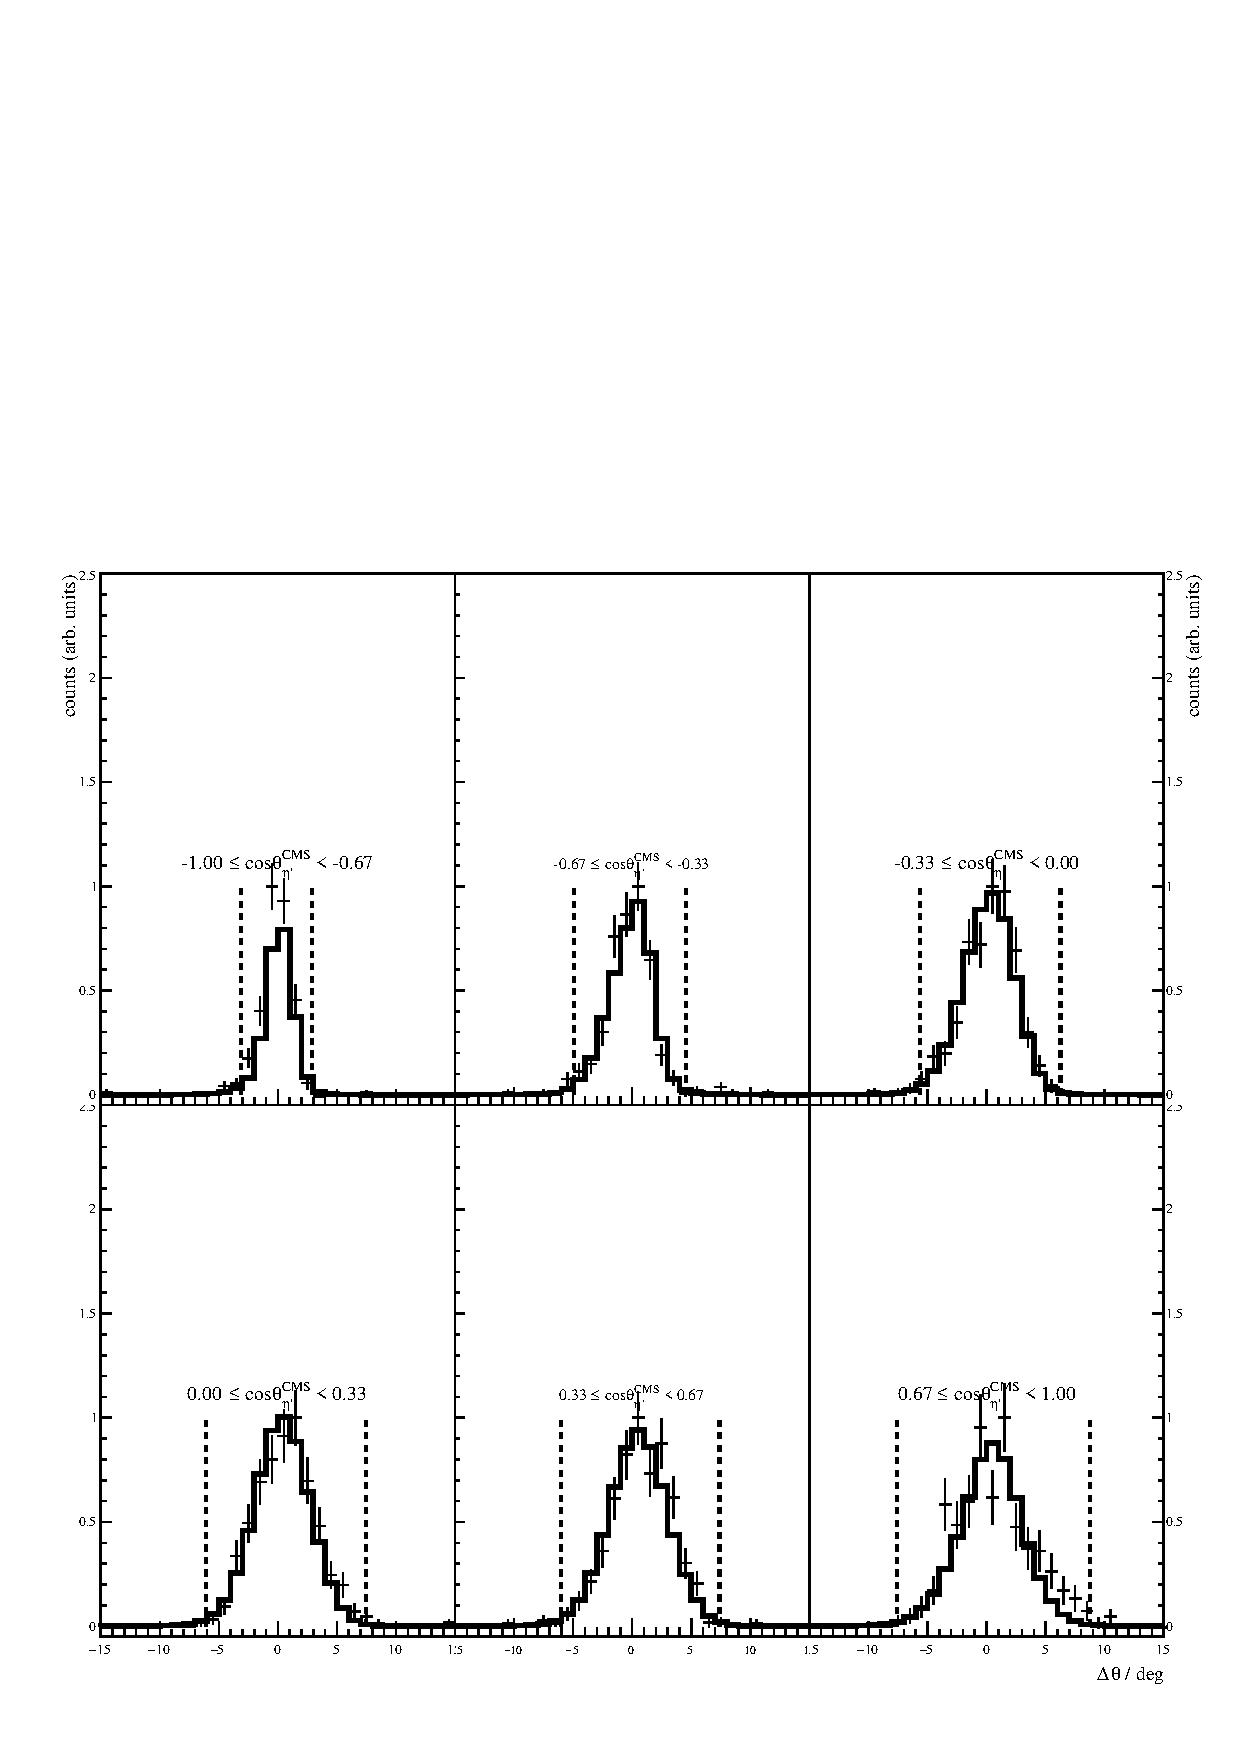
\includegraphics[width=\linewidth]{../figs/hydrogen/bin_cuts/thetacut_ebin1.pdf}
 	\caption{Polar angle difference of the $p\eta'$ final state with all other cuts applied for the energy bin $\SI{1500}{\mega\eV}\leq E_\gamma<\SI{1600}{\mega\eV}$. The vertical dashed lines show the cut ranges obtained from a gaussian fit to the data (open circles). The solid black histograms represent fitted MC data of $\eta'\to\gamma\gamma$}
 	\label{fig:pol}
 \end{figure}
 \subsubsection{Missing mass}
 The missing mass spectra allow a first investigation of possible background reactions that pass event selection. For all angular bins of the first energy bin the missing mass is shown in figure \ref{fig:mism}; again, the open circles are the data points with corresponding statistical error bars. The solid colored histograms are fitted MC spectra of different possible background contributions while the black histogram is the signal contribution of $\eta'\to\gamma\gamma$ photoproduction. The turquoise histogram is the sum of all MC histograms. Generally, most of the data can be described by the $\eta'$ MC alone, but especially towards higher masses (and higher beam energies) background contributions extend the missing mass peak as flat background. These are reactions where the reconstructed meson mass $m_\text{meson}^2=E_\text{meson}^2-\vec{p}_\text{meson}^2$ is smaller than the $\eta'$ mass, resulting in larger values for the missing mass. Judging from the fit to the missing mass, $2\pi^0$ and/or $\pi^0\eta$ photoproduction may describe the background as both show similar shapes. All other previously mentioned reactions (table \ref{tab:mc}) do not contribute significantly. Better conclusions can be drawn from the invariant mass spectra as is discussed in the following section \ref{sec:bkg}. The cut ranges for the missing mass are obtained from a \textsc{Novosibirsk} \cite{nov} fit to the data since the missing mass distribution is slightly asymmetric. However, since the tail parameter is small, still a symmetric cut of $\pm2\sigma$ was chosen. It was chosen narrower than the angular cuts to collect less background reactions.
  \begin{figure}[htbp]
 	\centering
 	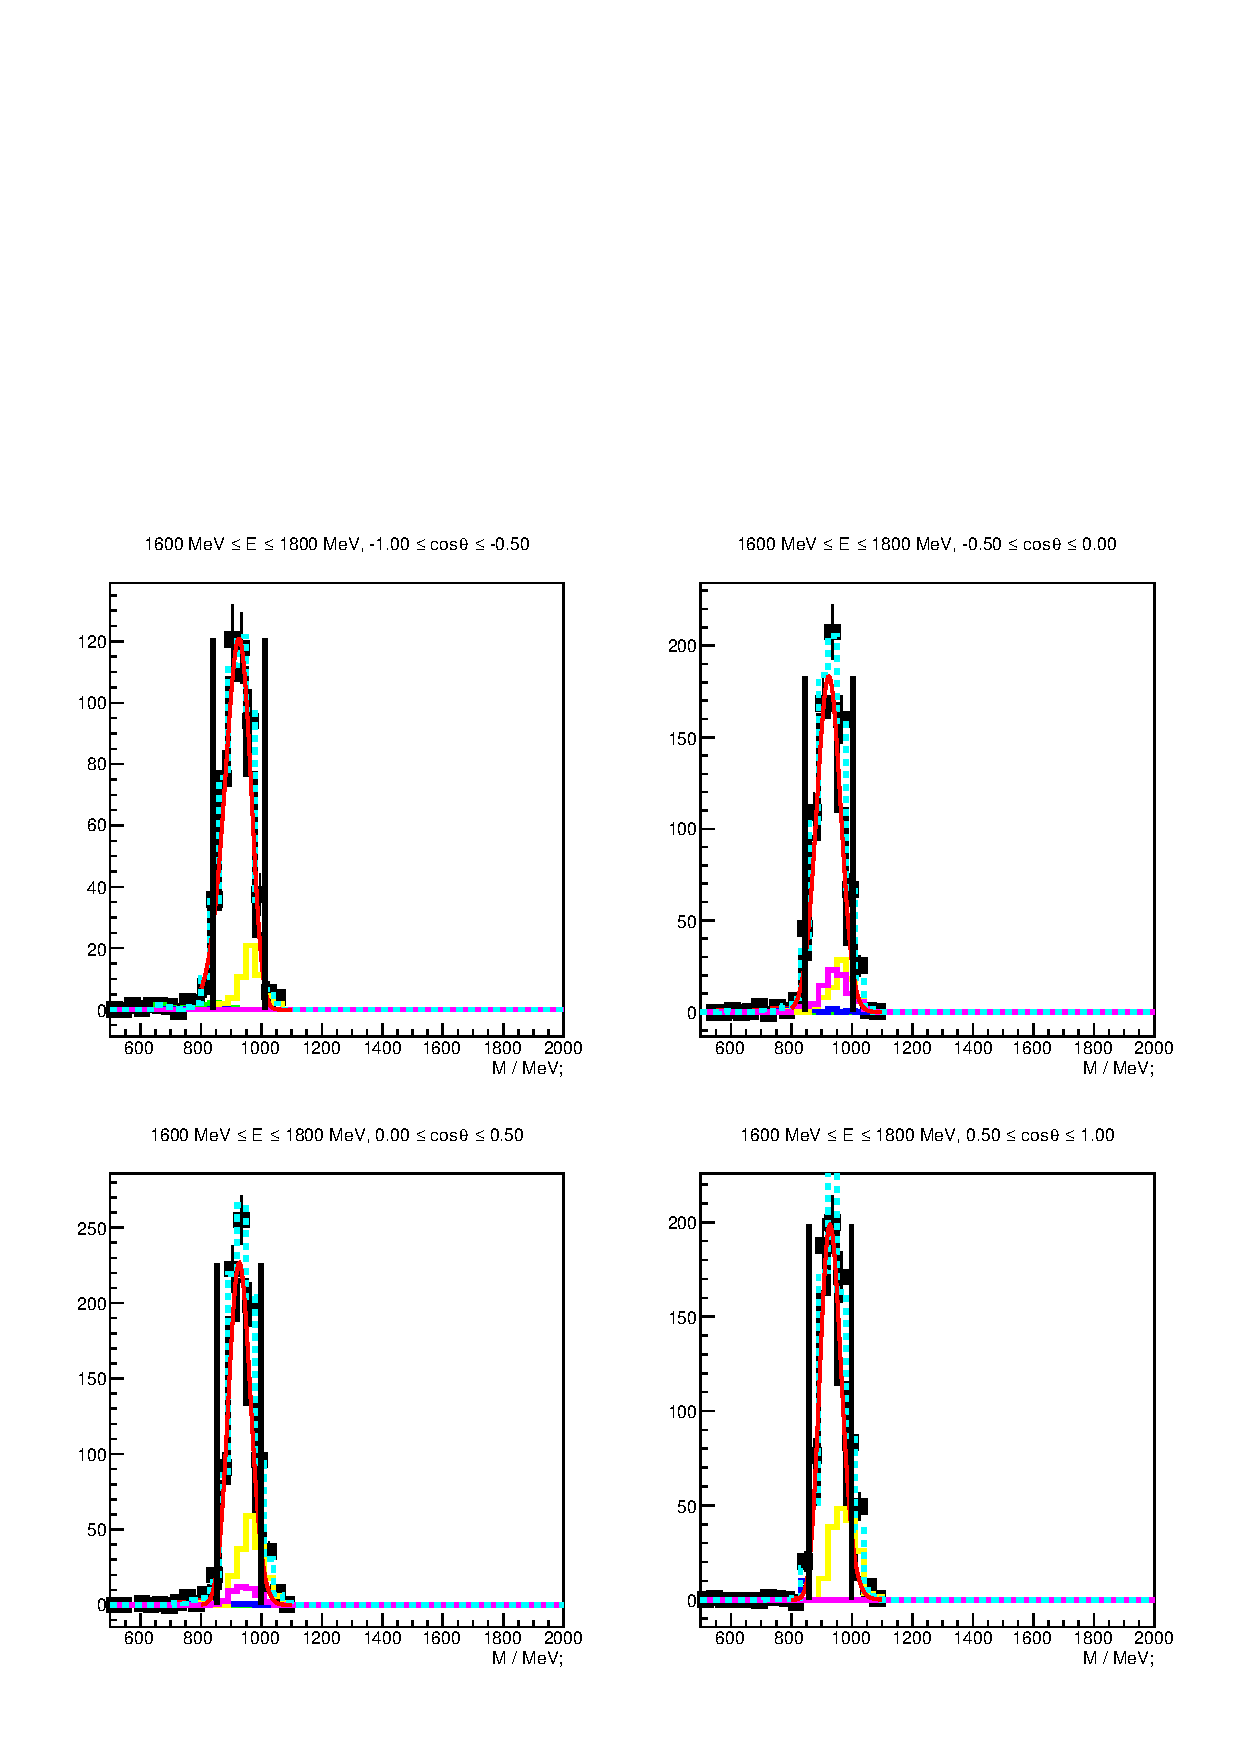
\includegraphics[width=\linewidth]{../figs/hydrogen/bin_cuts/mismcut_ebin1.pdf}
 	\caption{Missing mass of the $p\eta'$ final state with all other cuts applied for the energy bin $\SI{1500}{\mega\eV}\leq E_\gamma<\SI{1600}{\mega\eV}$. The vertical dashed lines show the cut ranges obtained from a fit to data (open circles) employing a \textsc{Novosibirsk} function. The solid colored histograms represent fitted MC data from relevant  photoproduction reactions: in black $\eta'$, in green $\pi^0$, in red $\eta$, in blue $\omega$, in yellow $2\pi^0$, magenta $\pi^0\eta$. The turquoise histogram is the sum of all MC histograms.}
 	\label{fig:mism}
 \end{figure}
 \subsubsection{Invariant mass}
 Investigating the invariant mass spectrum of the final state photons allows to illustrate the impact of the event selection so far. As has been mentioned all cuts considered up to this point apply to arbitrary meson photoproduction. This means that the invariant mass spectrum will depict peaks belonging to mesons produced in the considered beam energy range. This is shown in figure \ref{fig:globalinv} giving an overview over all energy and angular bins. All other cuts have been applied. The open circles represent data points and the different colored histograms MC data from relevant competing final states while the black histogram shows the signal contribution of $\eta'$ MC. The turquoise histogram is the sum of all MC contributions and describes the data very well. It has again been found that no other than the shown final states contribute significantly or improve the description of data by MC spectra. As expected one can observe peaks belonging to $\pi^0,\eta, \omega$ and $\eta'$ photoproduction. A flat background underneath the complete spectrum is realized by $2\pi^0$ and $\pi^0\eta$ final state photons that have been wrongfully combined to two photons. Remarkably, the $\pi^0,\eta$ and $\omega$ invariant mass distributions also depict long tails towards lower and higher masses, although they contribute only marginally to the sum of all MC spectra (note the logarithmic y-Scale). They can be explained by the fact that one low energetic photon is lost during reconstruction while the (high energetic) proton wrongfully creates two tracks of which one is then combined with the other photon as meson candidate \cite{farahphd}.
 \begin{figure}[htbp]
	\centering
	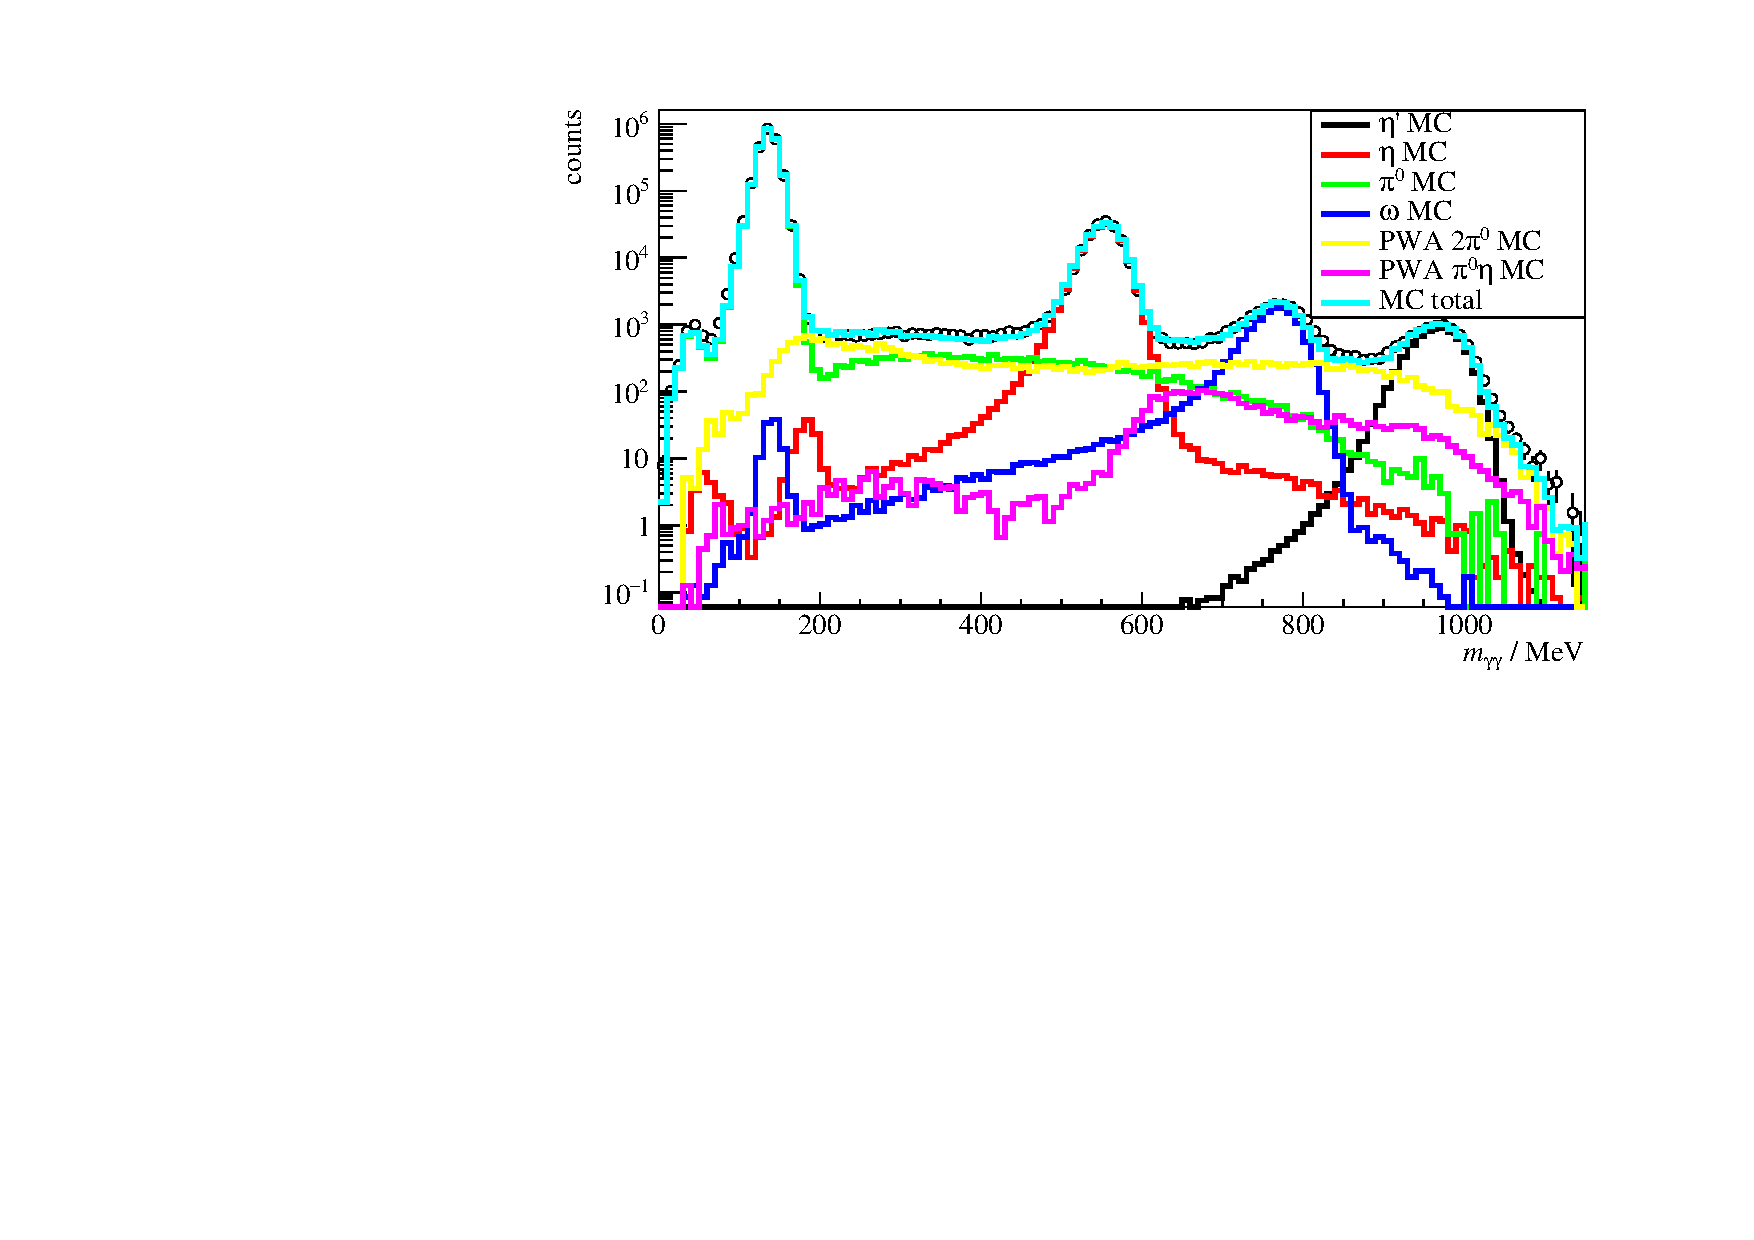
\includegraphics[width=\linewidth]{../figs/hydrogen/invm_global.pdf}
	\caption{Invariant mass of the $p\eta'$ final state with all other cuts applied for all energy and angular bins. The open circles represent the measured data, the solid colored histograms fitted MC data from relevant photoproduction reactions: in black $\eta'$, in green $\pi^0$, in red $\eta$, in blue $\omega$, in yellow $2\pi^0$ and in magenta $\pi^0\eta$. The turquoise histogram is the sum of all MC histograms.}
	\label{fig:globalinv}
\end{figure} 
To finally select only $\eta'$ photoproduction event candidates the invariant mass cut is determined again in bins of beam energy and meson polar angle. This is shown in figure \ref{fig:invm} for the first energy bin with all angular bins. Here, the same color coding as before applies, but the range of the invariant mass has been reduced to only cover the $\eta'$ peak for visibility's sake. Additionally the cut ranges, representing a $2\sigma$ interval obtained from a gaussian fit to the $\eta'$ MC, are shown as dashed, red lines. Considering the statistics the MC spectra still describe the data well. It is found again that the significant background contributions in the invariant mass range of interest are given by $2\pi^0$ and $\pi^0\eta$ photoproduction.  
\begin{figure}[htbp]
 	\centering
 	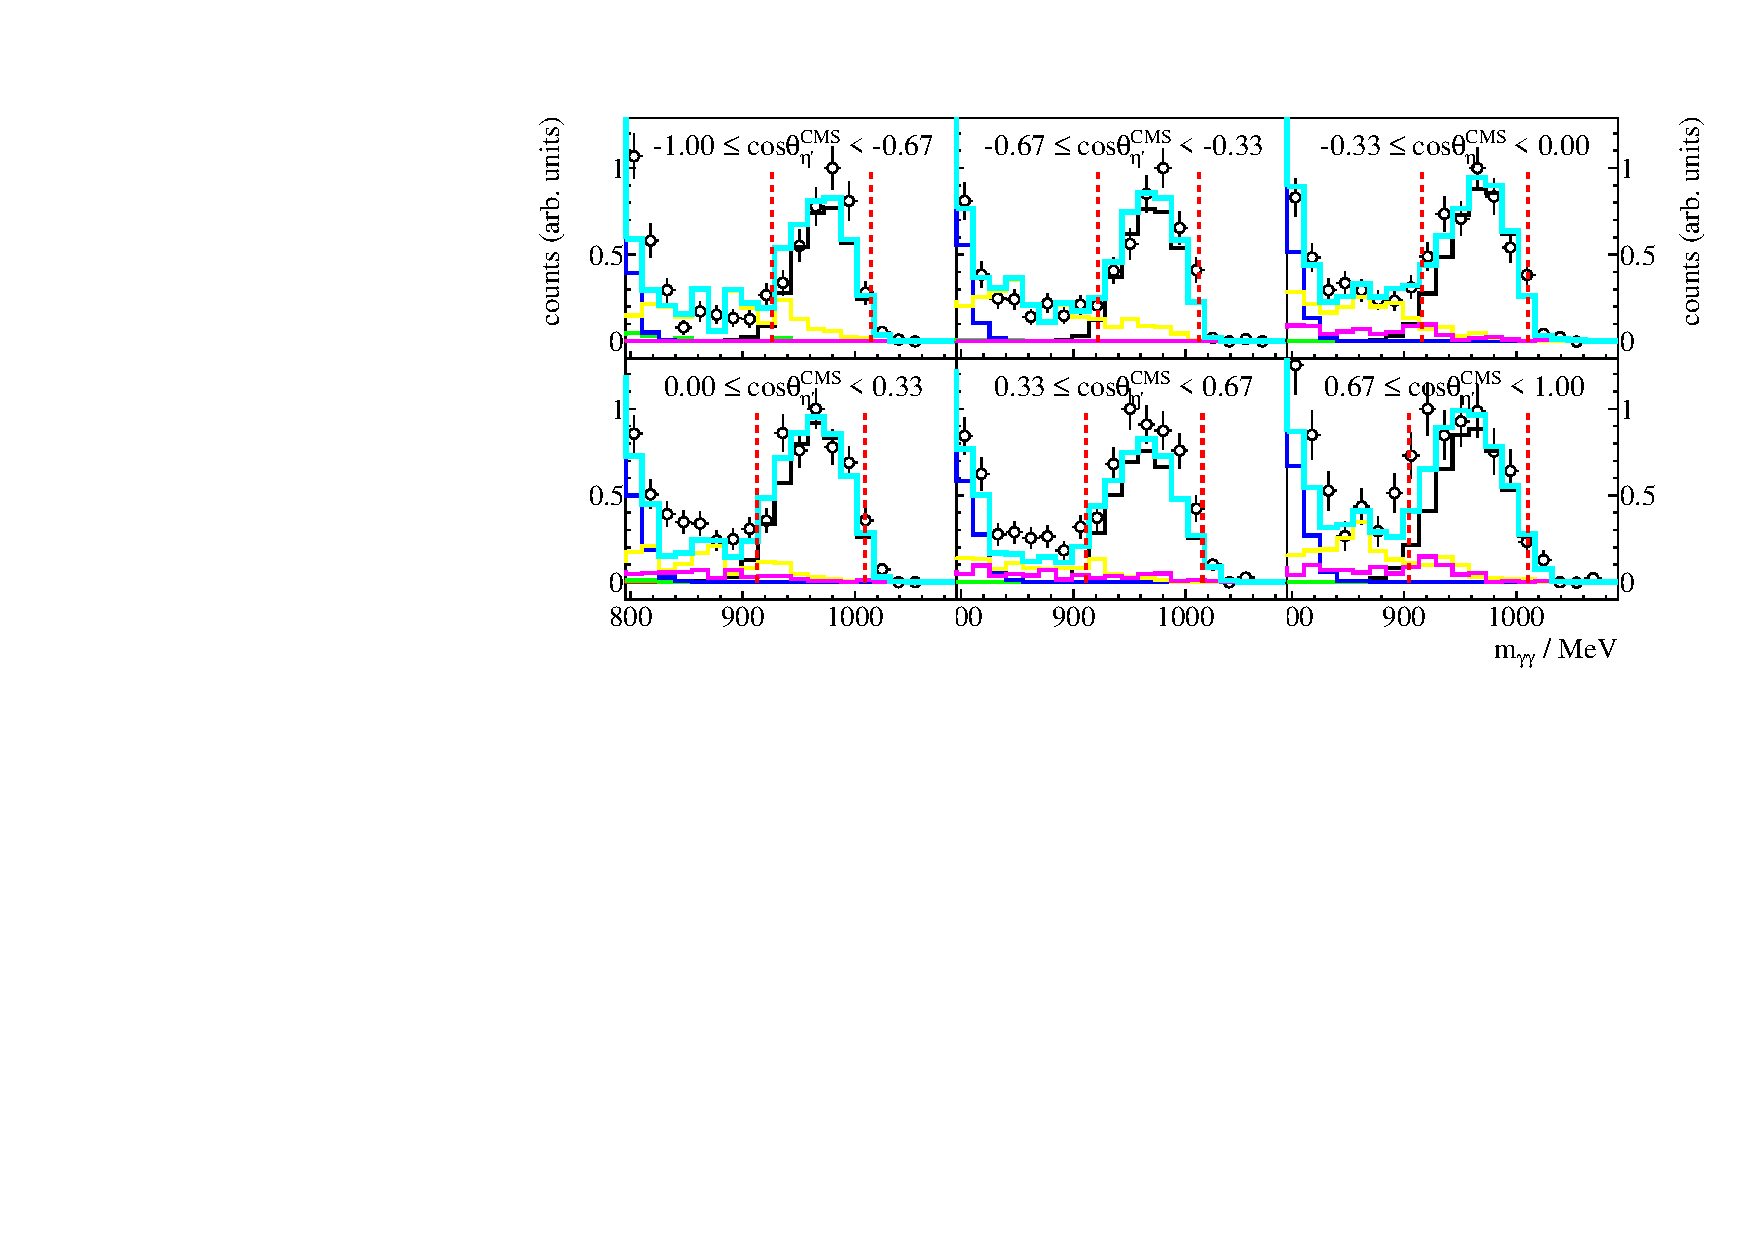
\includegraphics[width=\linewidth]{../figs/hydrogen/bin_cuts/invcut_ebin1.pdf}
 	\caption{Invariant mass of the $p\eta'$ final state with all other cuts applied for the energy bin $\SI{1500}{\mega\eV}\leq E_\gamma<\SI{1600}{\mega\eV}$. The vertical dashed lines show the cut ranges obtained from a gaussian fit to the $\eta'$ MC data (solid black histogram). The open circles represent the measured data, the solid colored histograms fitted MC data from relevant photoproduction reactions: in black $\eta'$, in green $\pi^0$, in red $\eta$, in blue $\omega$, in yellow $2\pi^0$ and in magenta $\pi^0\eta$. The turquoise histogram is the sum of all MC histograms.}
 	\label{fig:invm}
\end{figure}
\subsection{Quality of event selection}
In order to investigate the impact of applied cuts the detector and analysis acceptance $A(E_\gamma,\cos\theta)$ can be investigated. It is defined as the ratio of reconstructed events $N^\text{rec}(E_\gamma,\cos\theta)$ to generated events $N^\text{gen}(E_\gamma,\cos\theta)$ \begin{equation}
	A:=\frac{N^\text{rec}(E_\gamma,\cos\theta)}{N^\text{gen}(E_\gamma,\cos\theta)}
\end{equation}
and is shown in figure \ref{fig:acc}. Acceptance holes are visible in very forward and in backward direction which can be contributed to events where the proton escapes the calorimeters or is absorbed in insensitive material. Also, events close to threshold are unlikely to be reconstructed which can also be explained by low energy protons and/or low energy photons. A maximum acceptance of $\tilde{A}\approx0.61$ is reached which can be understood considering the cuts that have been made; each $3\sigma$ cuts retains $99\%$ of events and each $2\sigma$ cut $95\%$. Assuming detection efficiencies of $90\%$ for the two uncharged photons and $85\%$ for the charged proton (\cite{farahphd,hartmannphd}) it is evident that $0.99^2\cdot0.95^2\cdot0.9^2\cdot0.85\approx0.61$.
\begin{figure}[htbp]
	\centering
	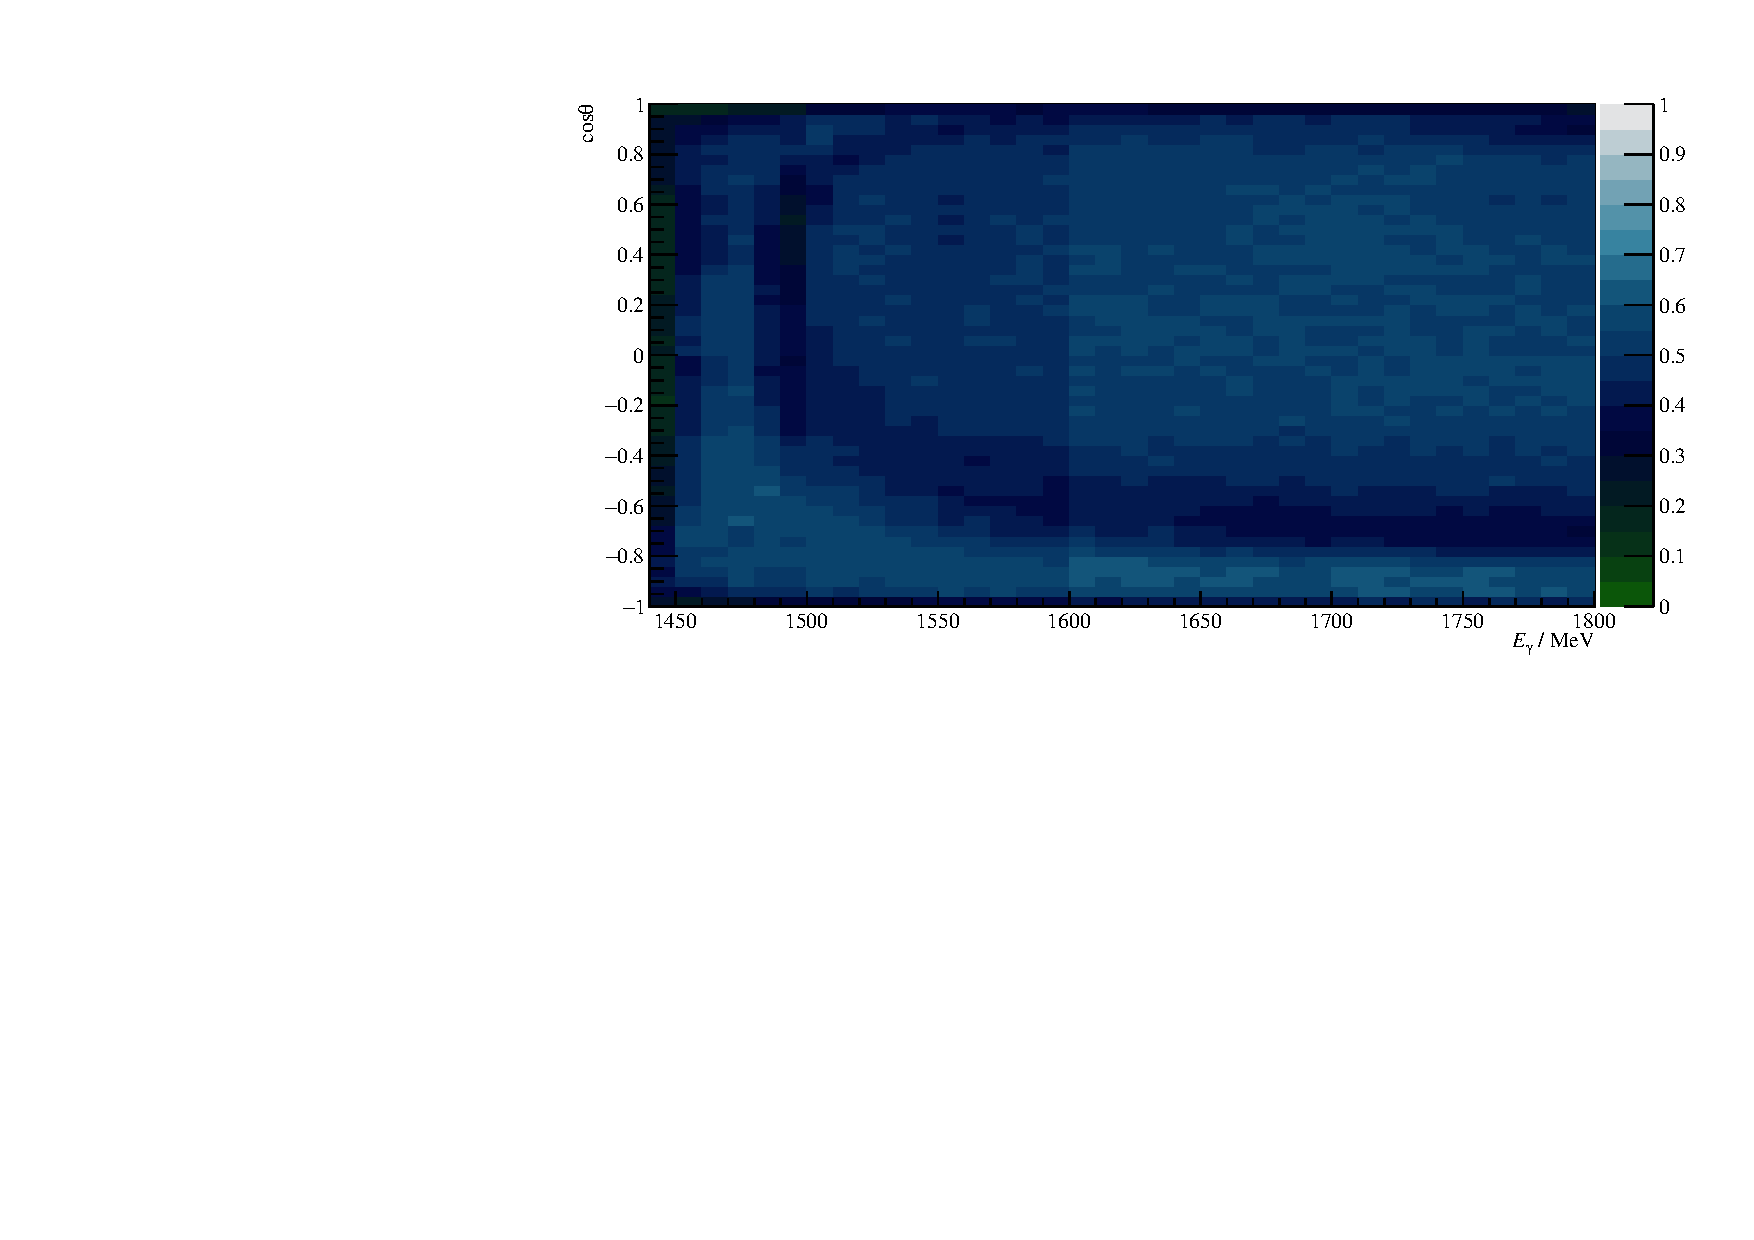
\includegraphics[width=\linewidth]{../figs/hydrogen/acceptance.pdf}
	\caption{Acceptance for the reaction $\gamma p\to p \eta'$ after all cuts that have been discussed so far for 2.5PED and 3PED events}
	\label{fig:acc}
\end{figure}
In total, $8\cdot10^3$ $\eta'$ events were extracted which nonetheless still contain background contaminations. In order to take this into account in the later analysis the fraction of background is determined for each bin in beam energy and meson polar angle. It is estimated as the fraction of background MC events to total MC events and shown in figure \ref{fig:bkg}. For most bins around $15\%$ of all events are misidentified as $\eta'$ events. Especially at very forward $\cos\theta\to1$ and backward $\cos\theta\to-1$ angles the background contributions are significantly higher, reaching up to $45\%$.
\begin{figure}[htbp]
	\centering
	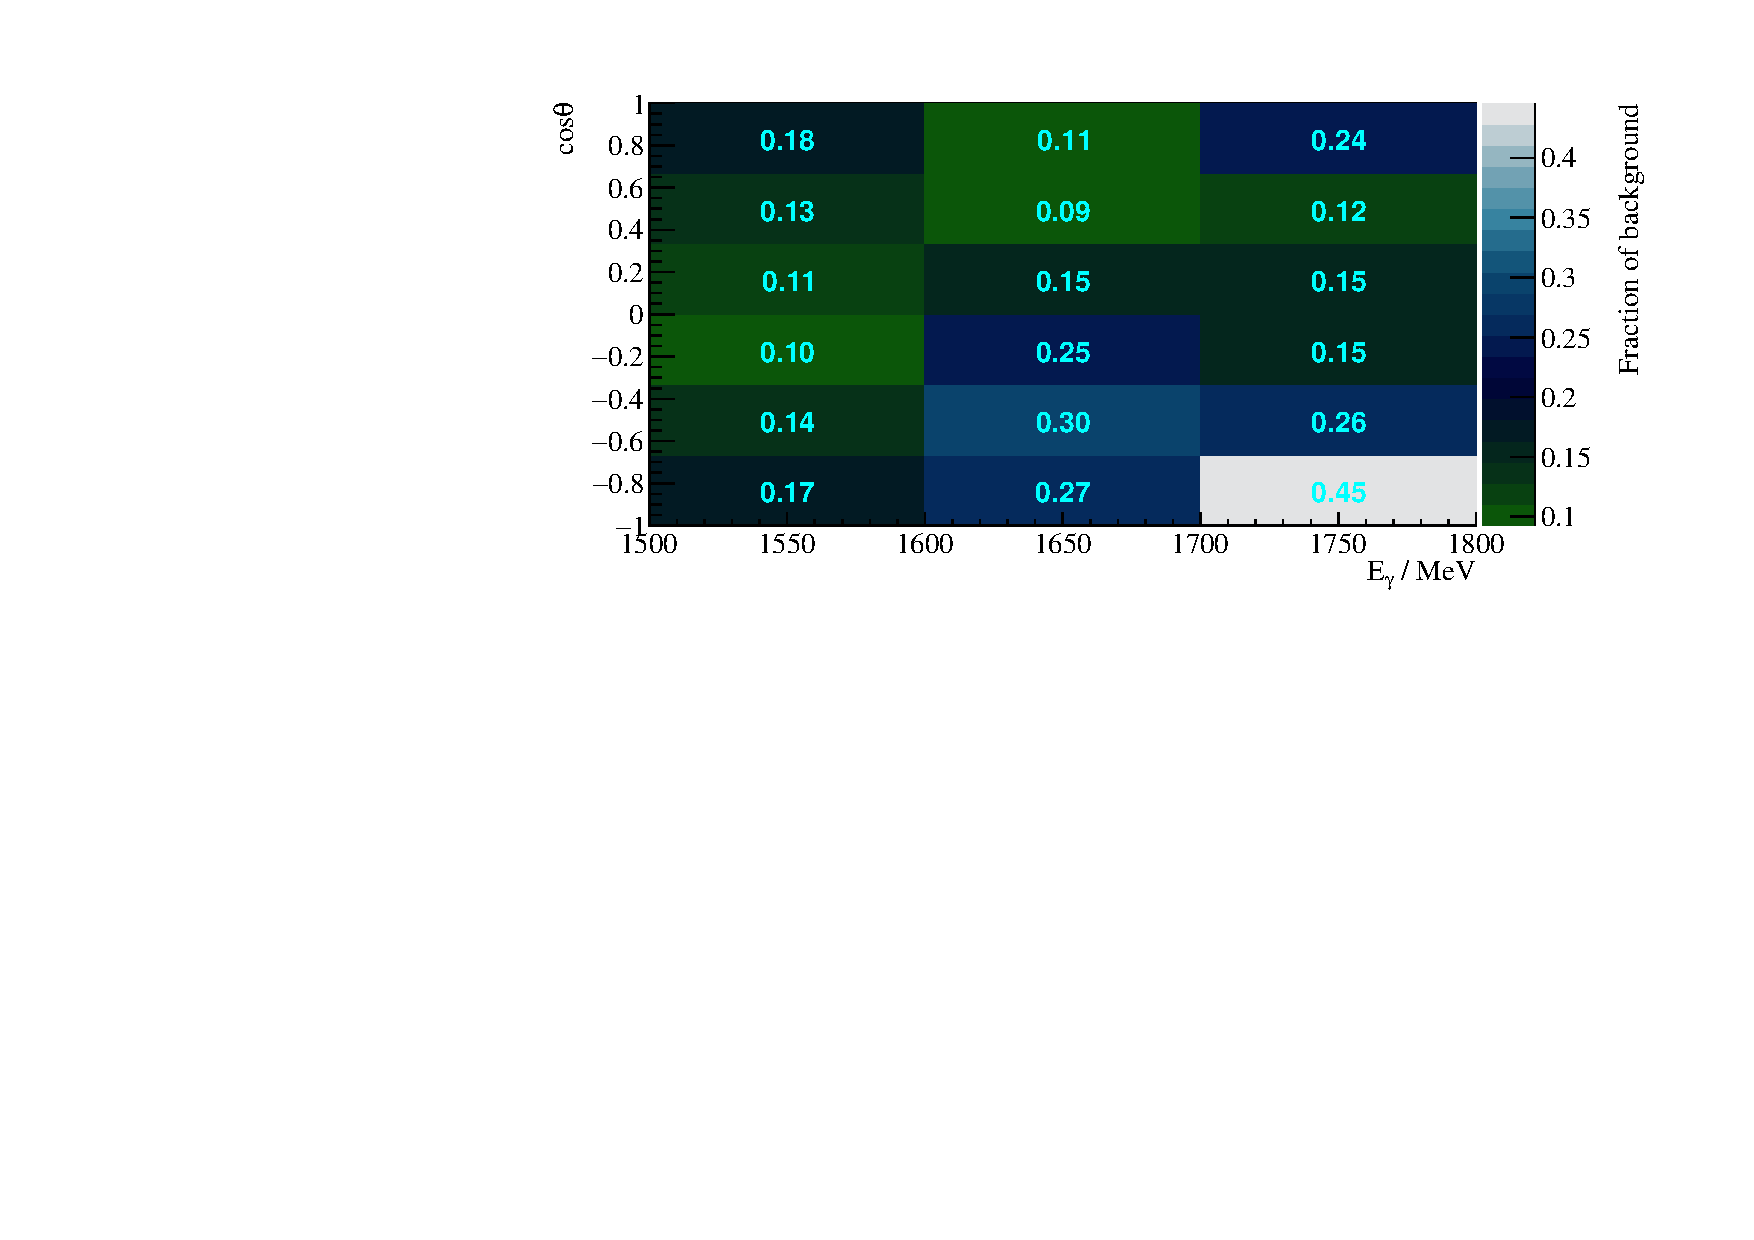
\includegraphics[width=\linewidth]{../figs/hydrogen/bin_cuts/invcut_bkg_percentage.pdf}
	\caption{Fraction of background events in the analyzed beam energy and angular bins.}
	\label{fig:bkg}
\end{figure}

\section{Investigation of background and additional cuts} 
\label{sec:bkg}
So far the background reactions in the $\eta'$ cut ranges have been discussed only phenomenologically as they describe the measured invariant mass spectra best. In the following the plausibility and causality of these background contributions shall be discussed. Furthermore it is investigated if the found background contributions may be reduced or eliminated by additional cut conditions.

\subsection{Inspecting plausibility of background reactions}
To evaluate the likelihood that the background contributions are made up of $2\pi^0$ or $\pi^0\eta$ production events the respective production cross sections in the inspected beam energy region and branching ratios (BR) to purely photonic final states are examined, see table \ref{tab:plausmc}. Also displayed is the maximum acceptance $\tilde{A}$ which is additionally shown in figure \ref{fig:acc_bkg}. Both possible background reactions exceed $\eta'$ photoproduction in cross section and also in relative frequency of purely photonic final states. At the same time the acceptance is almost vanishing, proving that the kinematic cuts are generally very effective. 

\begin{figure}[htbp]
	\centering
	\begin{subfigure}{\linewidth}
			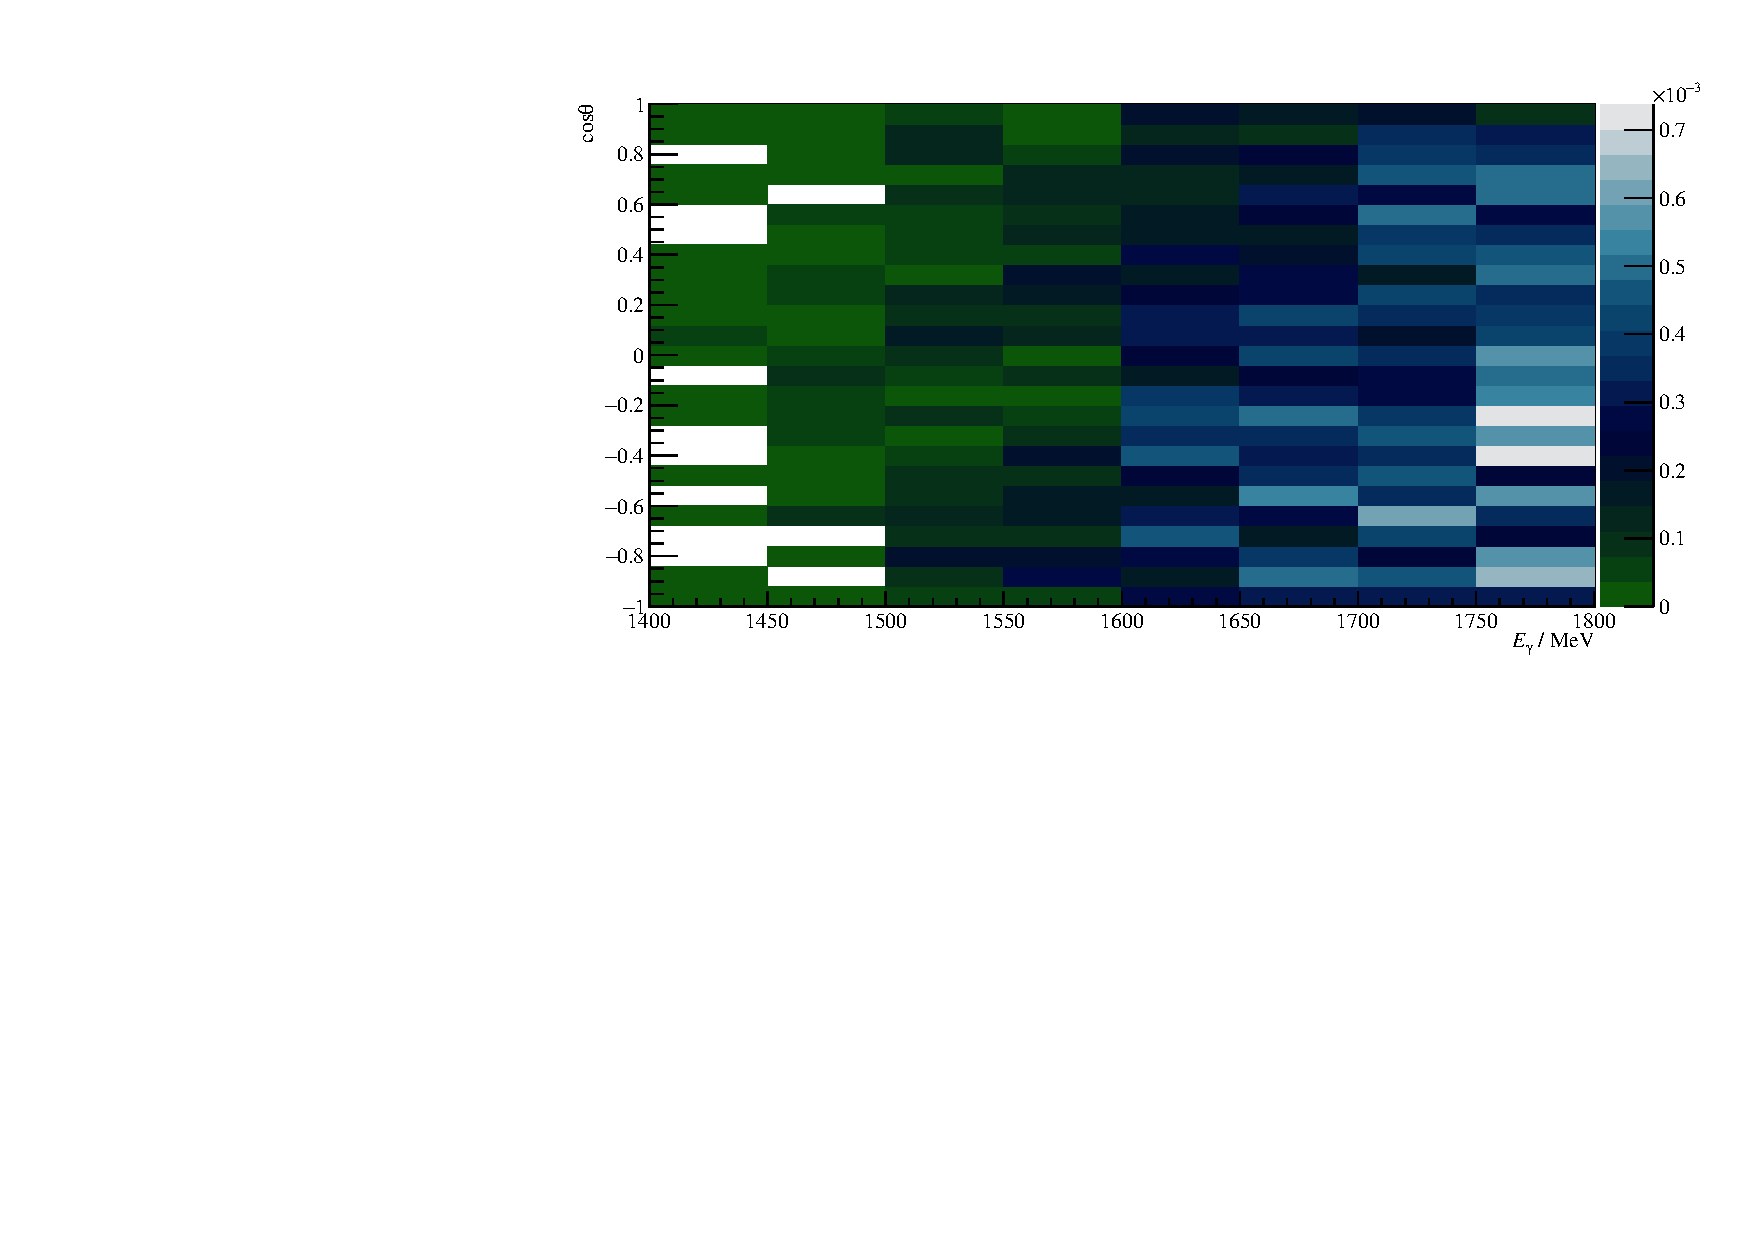
\includegraphics[width=\linewidth]{../figs/hydrogen/acceptance_2pi0.pdf}
			\subcaption{$\gamma p \to p 2\pi^0$}			
	\end{subfigure}
\begin{subfigure}{\linewidth}
		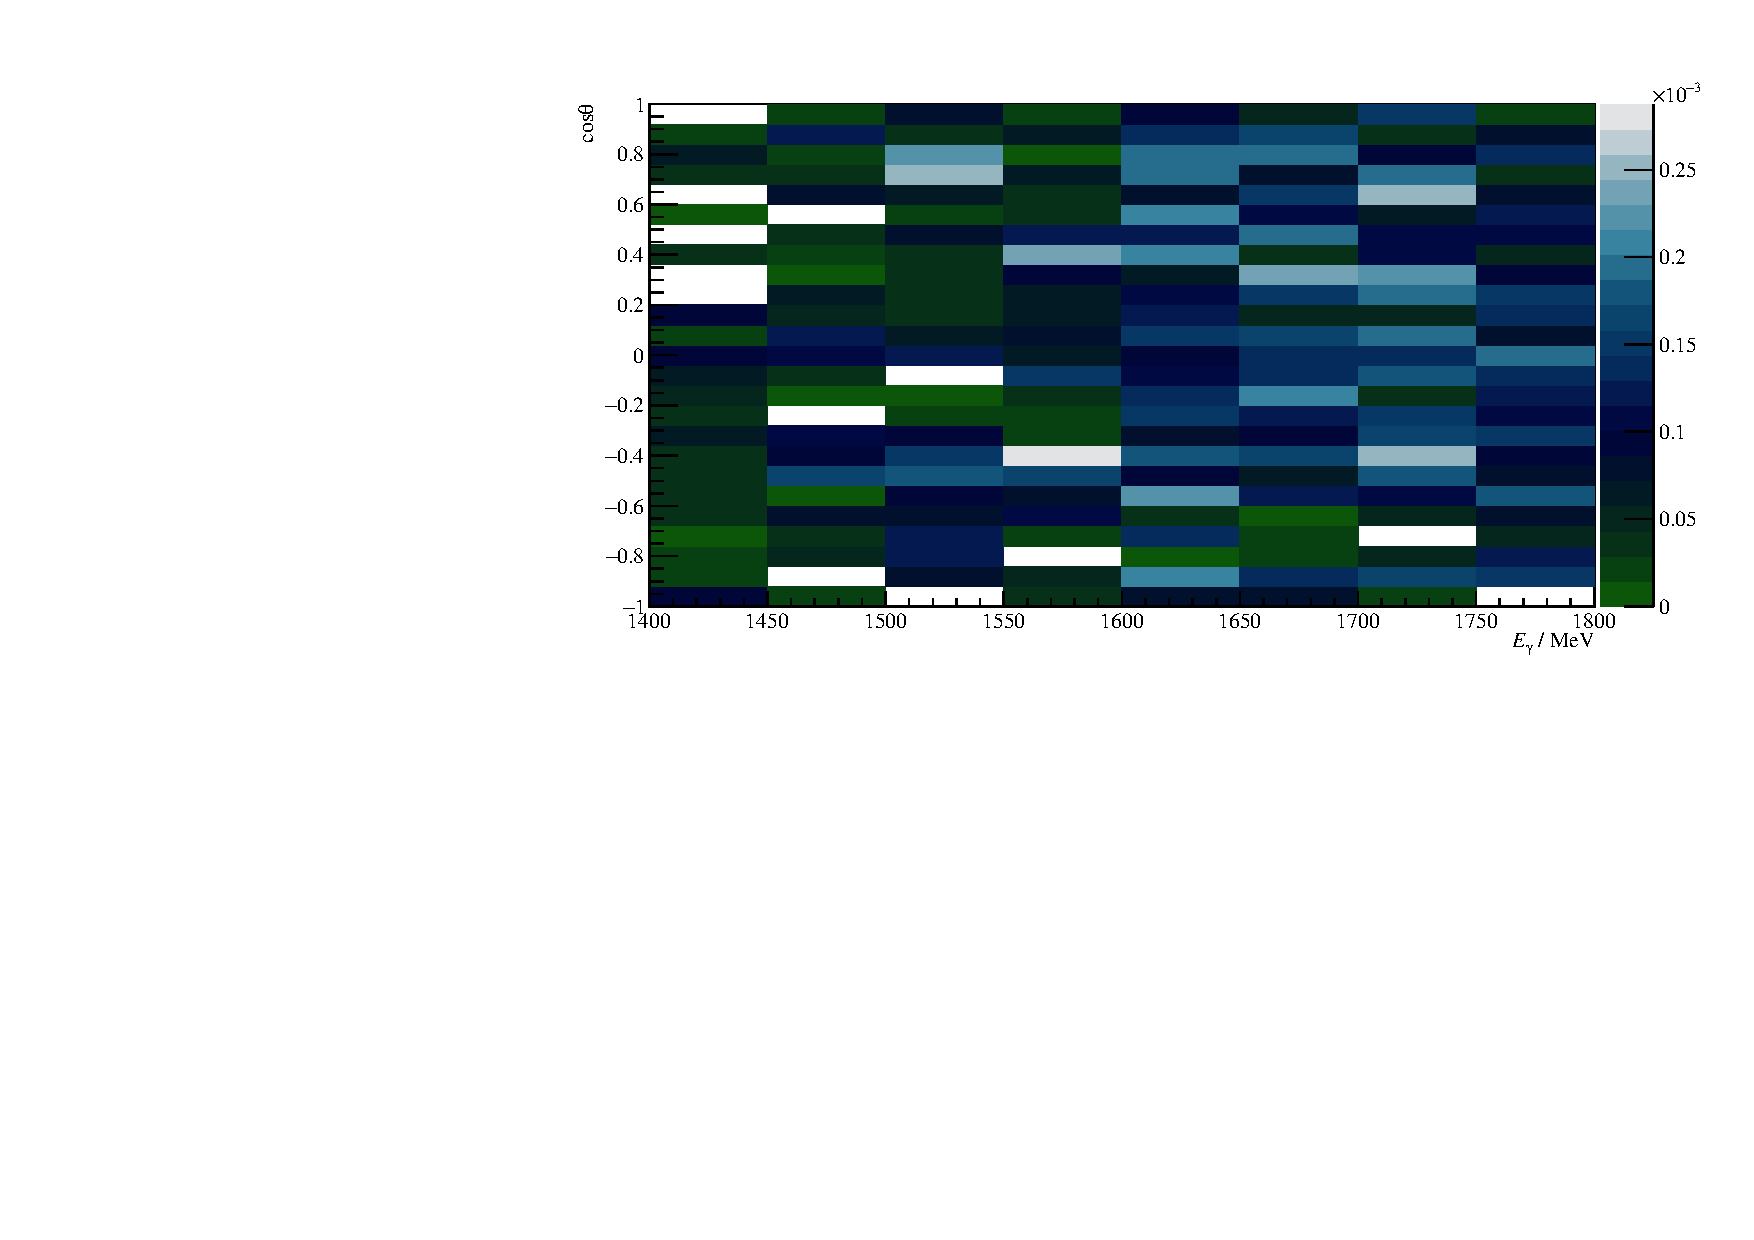
\includegraphics[width=\linewidth]{../figs/hydrogen/acceptance_pi0eta.pdf}
		\subcaption{$\gamma p \to p \pi^0\eta$}
\end{subfigure}
\caption{Acceptance for possible background contributions}
\label{fig:acc_bkg}
\end{figure}

\begin{table}[htbp]
	\centering
	\begin{tabular}{cccc}
		\toprule
		reaction & $\sigma$ / \si{\micro\barn} & BR to $n\gamma$ & $\tilde{A}$\\
		\hline
		$\gamma p\to p\eta'$ &$\approx1$ \cite{etap_cs}& $0.02$ & $0.61$\\
		$\gamma p\to p2\pi^0$ &$\lesssim5$ \cite{2pi0_cs}&$0.98^2=0.96$& $7\cdot 10^{-4}$\\
		$\gamma p\to p\pi^0\eta$ &$\approx3$ \cite{pi0eta_cs} &$0.98\cdot0.38=0.37$&$2\cdot 10^{-4}$\\
		\bottomrule 		
	\end{tabular}
\caption{Total cross sections $\sigma$ in the energy range \SIrange{1500}{1800}{\mega\eV}, branching ratios (BR) to $n\gamma$ final states and maximum acceptance $\tilde{A}$ for signal and possible background contributions}
\label{tab:plausmc}
\end{table}


Since the total number of events is proportional to the cross section $\sigma$, branching ratio BR and acceptance $\tilde{A}$, the ratio of reconstructed background to signal events is then given by $$R=\frac{\sigma\cdot\text{BR}\cdot\tilde{A}}{\sigma_{\eta'}\cdot\text{BR}_{\eta'\to\gamma\gamma}\cdot\tilde{A}_{\eta'}}=\frac{\sigma\cdot\text{BR}\cdot\tilde{A}}{\SI{1}{\micro\barn}\cdot0.02\cdot0.61}.$$
One finds $R\lesssim0.3$ and $R\lesssim0.05$ for $2\pi^0$ and $\pi^0\eta$ photoproduction, respectively. Although less than $0.1\%$ of two meson production reactions are misidentified as $\eta'$ events they make up a significant portion of background in $\eta'$ data, as considering the according branching ratios and cross sections showed. Furthermore, the previous empirical assumption to only include $2\pi^0$ and $\pi^0\eta$ MC in the fit to describe the data is now justified since the found background percentages agree well with the now motivated upper boundaries.    
\newpage
\subsection{Misidentification of background reactions}
It has been reasonably established that the main background reactions that escape the $\eta'$ event selection cuts are realized by $2\pi^0$ and $\pi^0\eta$ production. However, it remains to explain why a four-photon final state is misidentified as $\eta'$ event. In order to do so the MC simulations of the respective final states were investigated. One observes that for those events that passed the $\eta'$ cuts the generated photon energies for two photons often were of order $E_{\gamma,i} \sim \mathcal{O}(\SI{10}{\mega\eV})$ and the other two of order $E_{\gamma,i} \sim \mathcal{O}(\SI{100}{\mega\eV})$. The reconstructed energies however only displayed energies of order $E_{\gamma,i} \sim \mathcal{O}(\SI{100}{\mega\eV})$.  During the reconstruction of final state four momenta, a minimum energy of $\SI{20}{\mega\eV}$ per cluster is demanded in order to suppress electromagnetic background. This threshold is not passed or only closely passed by both lowest energy final state photons of $2\pi^0$ production for $\sim 60\%$ of all events, see figure \ref{fig:mcgammas_a}.\begin{figure}[htbp]
	\centering
	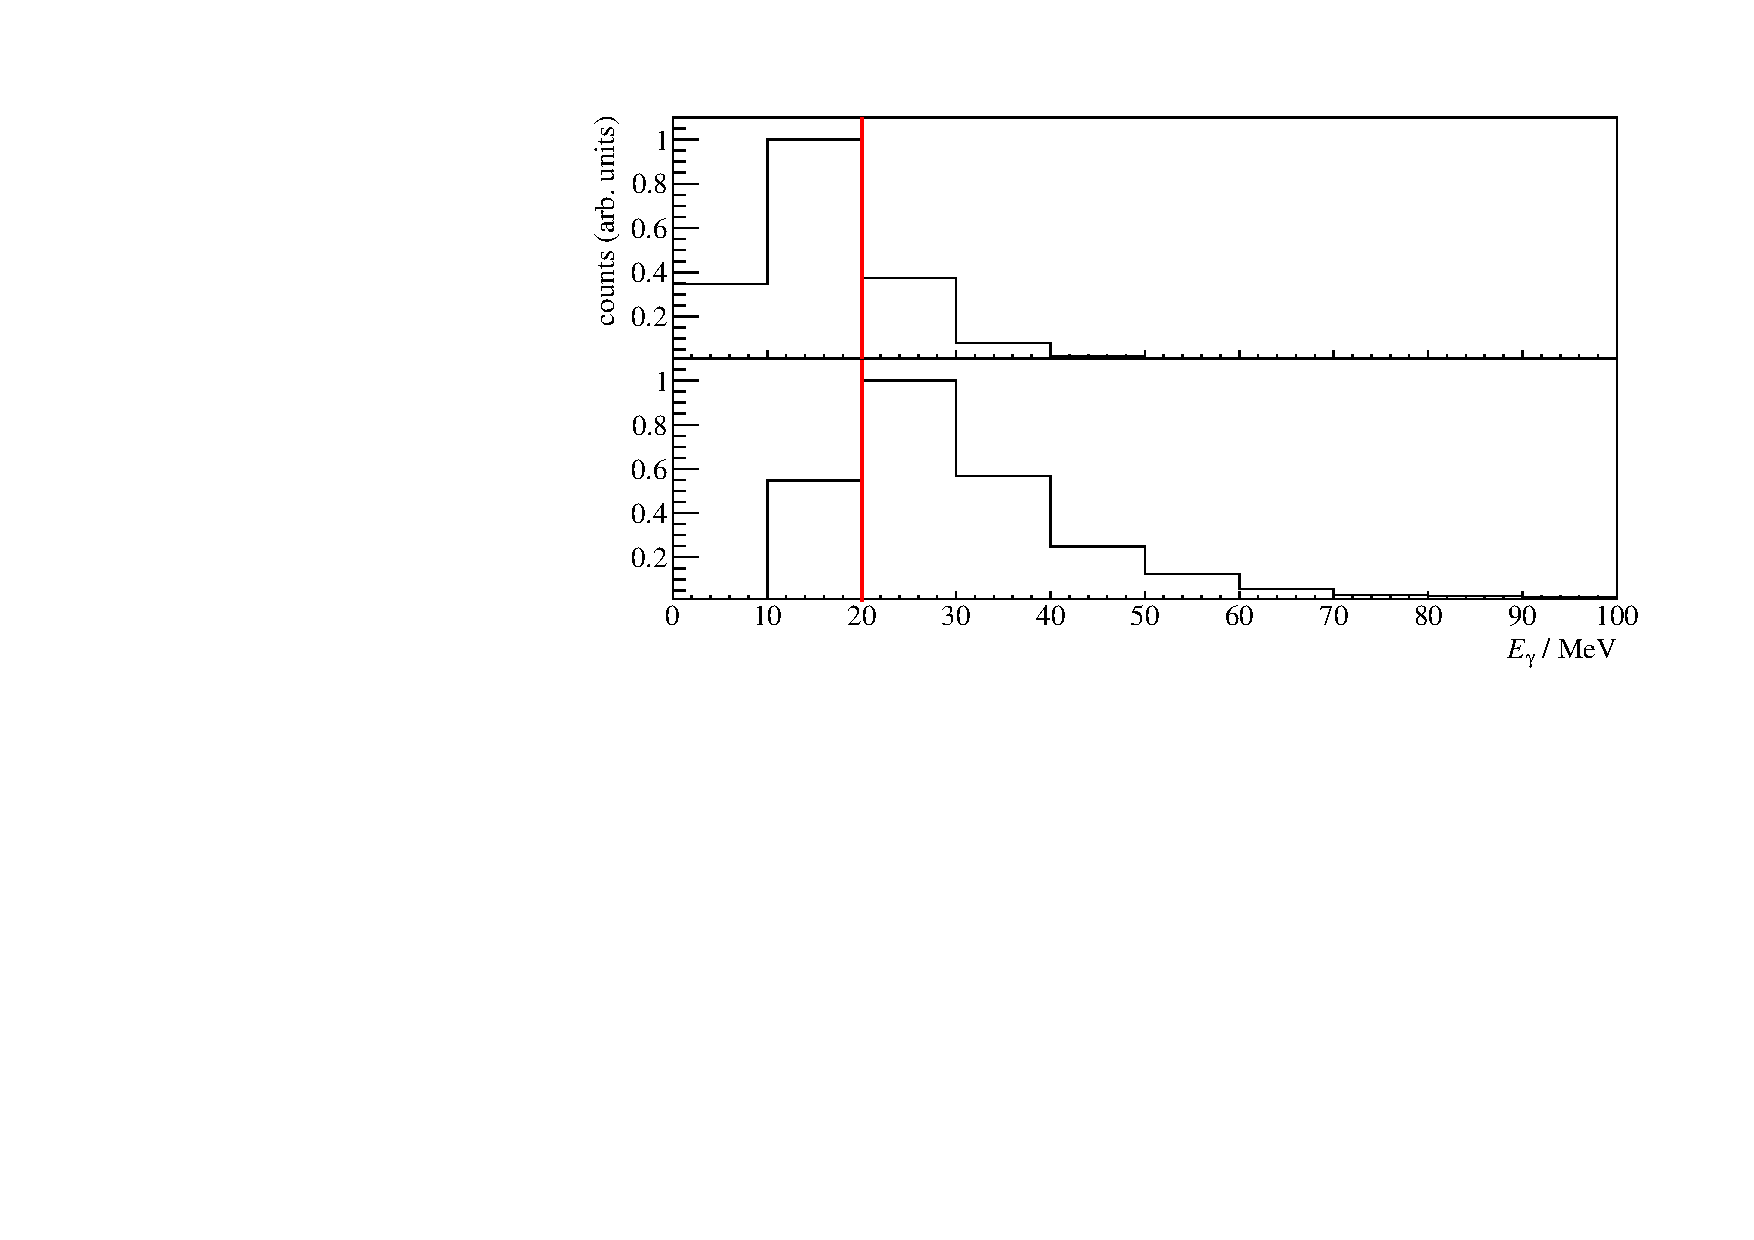
\includegraphics[width=\linewidth]{../figs/hydrogen/mcgammas.pdf}
	\caption{Generated energies of the two lowest energy photons in $2\pi^0$ photoproduction MC data. The threshold of $\SI{20}{\mega\eV}$ is marked by a vertical red line. Lowest energy photon is shown on the top, second lowest energy photon is shown on the bottom.}
	\label{fig:mcgammas_a}			
\end{figure}
 Similarly, $\sim70\%$ of $\pi^0\eta$ events have a final state photon which does not or only closely pass the threshold of $\SI{20}{\mega\eV}$. Other than in $2\pi^0$ reactions, this does only apply for one of the lowest energy photons while the other significantly exceeds the threshold of $\SI{20}{\mega\eV}$, see figure \ref{fig:mcgammas_b}. 
 \begin{figure}[htbp]
 	\centering
 	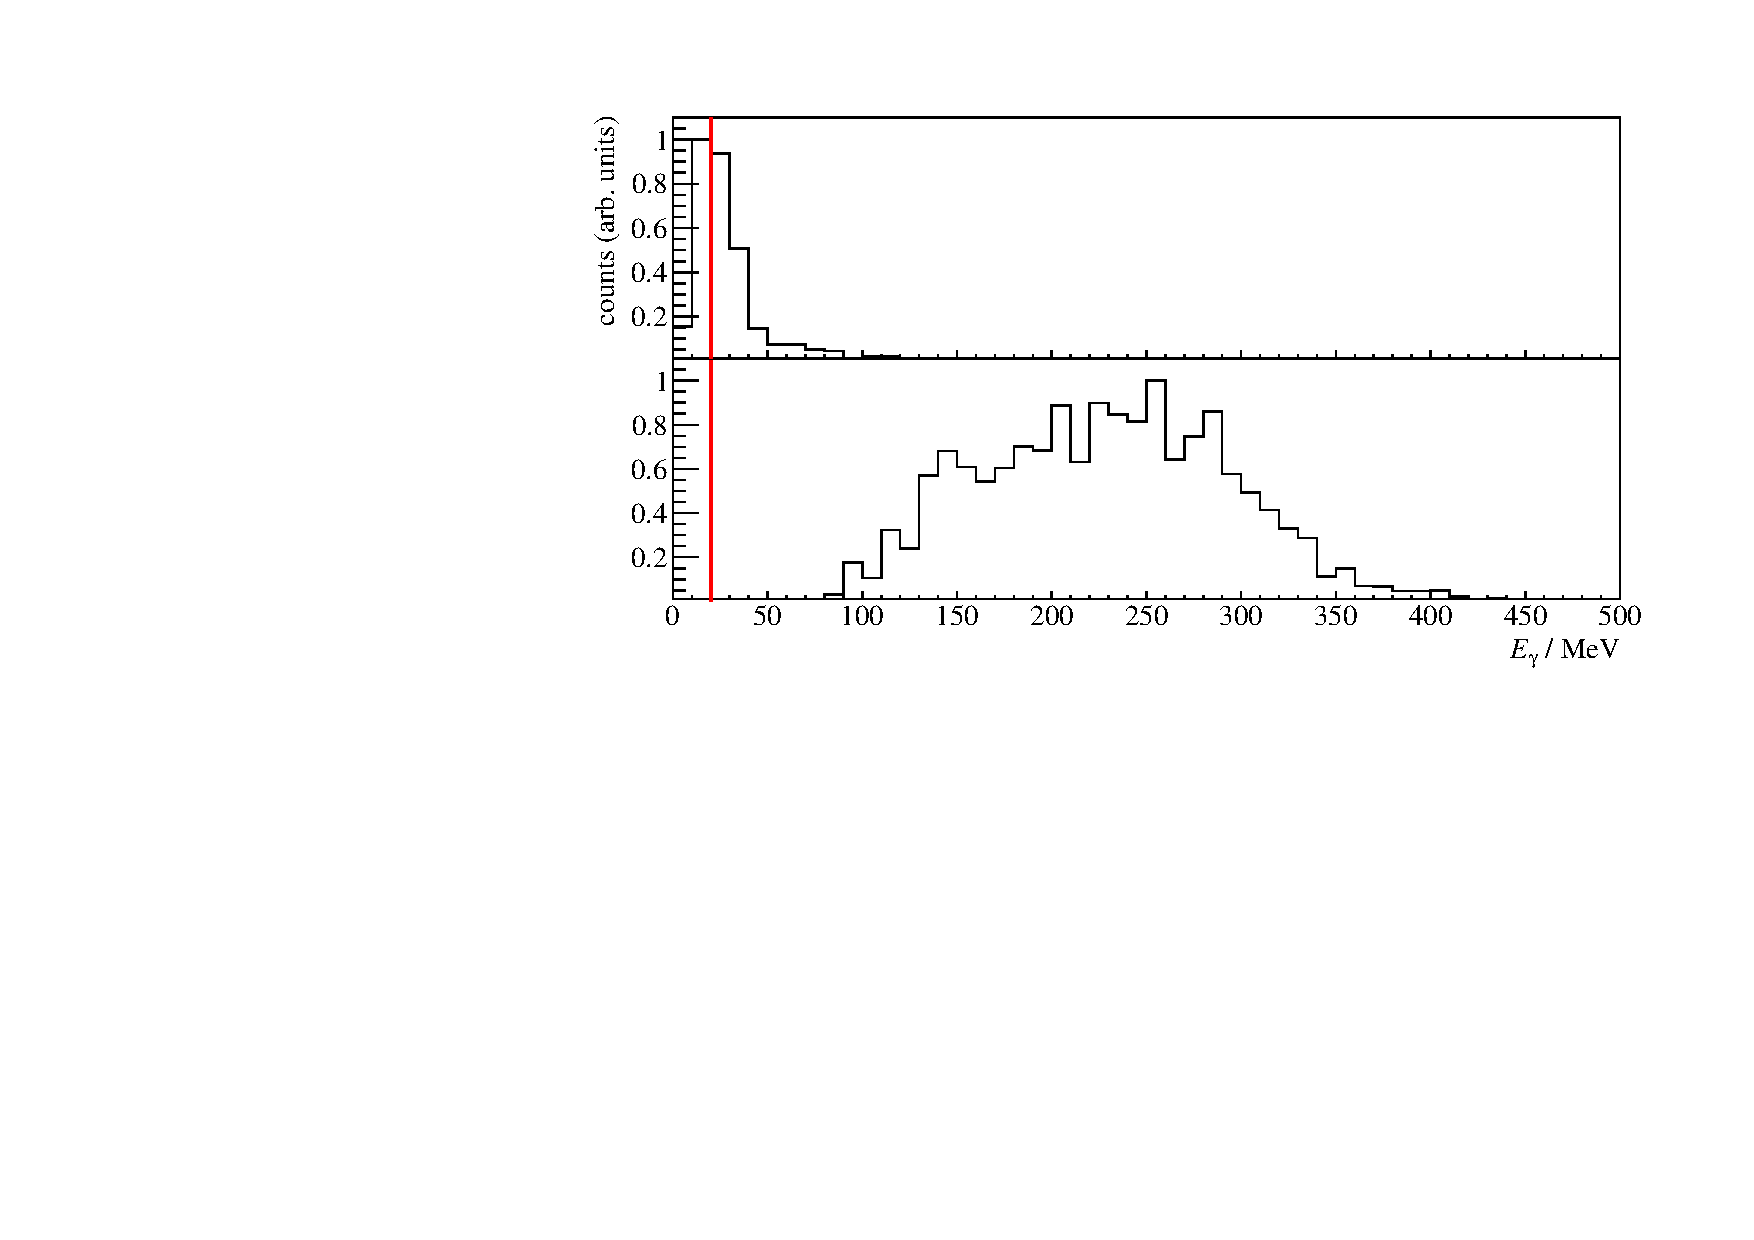
\includegraphics[width=\linewidth]{../figs/hydrogen/mcgammas_pi0eta.pdf}
 	\caption{Generated energies of the two lowest energy photons in $2\pi^0$ and $\pi^0\eta$ photoproduction MC data. The threshold of $\SI{20}{\mega\eV}$ is marked by a vertical red line. Lowest energy photon is shown on the top, second lowest energy photon is shown on the bottom.}
 	\label{fig:mcgammas_b}			
 \end{figure}
 Those photons with an energy above threshold may still be lost during reconstruction because they are falsely combined to one cluster with one of the two highest energy photons as a investigation of photon directions revealed; figure \ref{fig:mcangle} shows the polar angle difference between the second lowest energy photon and the second highest energy photon of the MC $\pi^0\eta$ final state which clearly peaks centered at $0$. 
\begin{figure}[htbp]
	\centering
	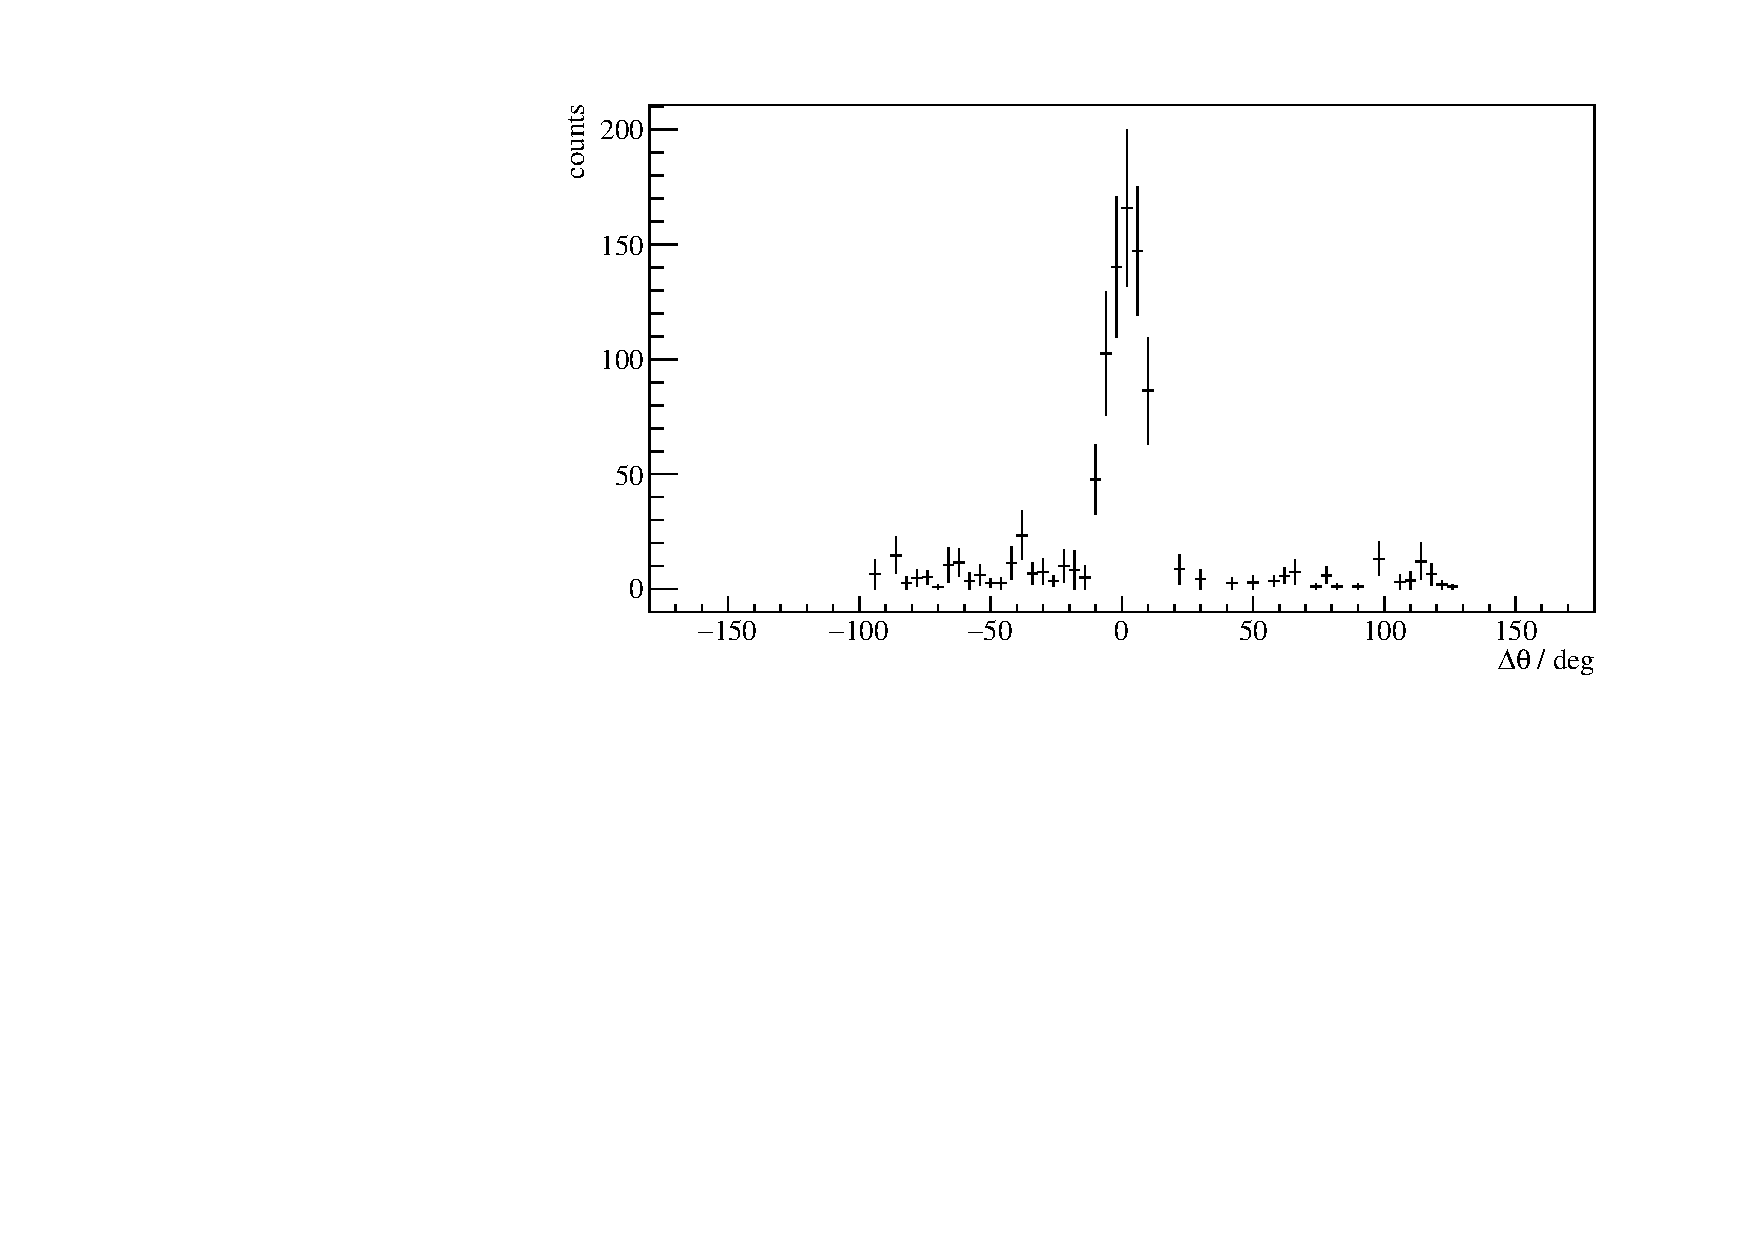
\includegraphics[width=\linewidth]{../figs/hydrogen/mcgammas_td_pi0eta.pdf}
	\caption{Polar angle difference $\Delta\theta$ between the photon with second highest energy and second lowest energy of the $\pi^0\eta$ final state.}
	\label{fig:mcangle}
\end{figure}
Similar results are found with $2\pi^0$ production events. It is evident that neither the two lost photons, nor the two reconstructed photons are correlated, i.e. decay products of the same meson.
\newpage
Considering the above one can now say that $2\pi^0$ and $\pi^0\eta$ events pass the $\eta'$ event selection because 
\begin{enumerate}
	\item two uncorrelated low energy photons are lost during reconstruction and the remaining two pass the kinematic cuts by chance, since they too are uncorrelated (see figure \ref{fig:mcgammas1}),

	\item one low energy photon is lost. Two of the remaining three photons are combined to one in favor of the higher energetic photon since they were emitted in the same direction. The two reconstructed photons are uncorrelated and pass the event selection randomly, as shown in figure \ref{fig:mcgammas2}.
\end{enumerate} 
	\begin{figure}[h]
	\centering
	\begin{subfigure}{.49\linewidth}
		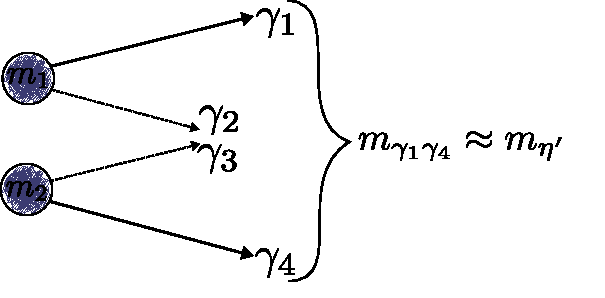
\includegraphics[width=\linewidth]{../figs/inkscape/mcgammas1.pdf}
		\subcaption{Two photons get lost while the remaining two get falsely combined to form a $\eta'$ meson\\}
		\label{fig:mcgammas1}
	\end{subfigure}
	\begin{subfigure}{.49\linewidth}
		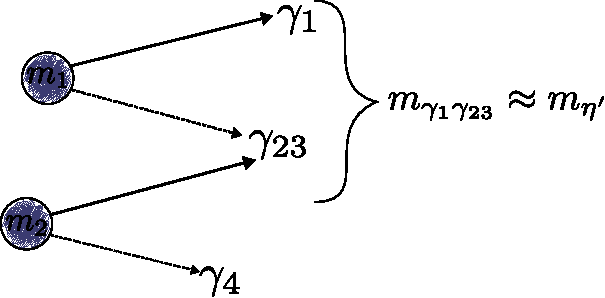
\includegraphics[width=\linewidth]{../figs/inkscape/mcgammas2.pdf}
		\subcaption{One photon gets lost, in addition two photons are grouped as one. The remaining two get falsely combined to form a $\eta'$ meson}
		\label{fig:mcgammas2}
	\end{subfigure}
	\caption{Illustration of the misidentification process during reconstruction}

\end{figure}
These claims are indeed further validated if one examines the polar angle that is reconstructed from the falsely assigned $\eta'$ candidates using the surviving two photon momenta. This can be compared to the generated polar angle that is built using all four final state photon momenta in the CMS $\mathbf{p}_{\gamma_i}$. They add up to the artificial two-meson momentum $\mathbf{p}_m$ which in the CMS has the same magnitude but opposite direction as the recoil proton with momentum $\mathbf{p}_\text{recoil}$
$$
	\mathbf{p}_m=\sum_{i=1}^4\mathbf{p}_{\gamma_i}=-\mathbf{p}_\text{recoil}.
$$ If the lost photons have very low energies and/or are emitted in the same direction as other photons one would expect the polar angle that is spanned by the four final state photons approximately agrees with the polar angle that is built using the two photons that survived event selection, such that $\cos\theta(4\gamma)\approx\cos\theta(2\gamma)$. This is exactly what is observed, as figure \ref{fig:mccostheta} shows for both background reactions: the generated CMS angle $\cos\theta_\text{gen.}$ is plotted against the reconstructed CMS angle $\cos\theta_\text{rec.}$. The events are clearly distributed around the slope $\cos\theta_\text{gen.}=\cos\theta_\text{rec.}$ which is indicated by the solid line. This is an important result for the later analysis: if the background contributions are taken into account quantitatively then the extracted beam asymmetry has to be corrected by the asymmetry stemming from background reactions. This is only possible if the background reactions from e.g. $2\pi^0$ events realize the same bins in beam energy and CMS angle as in a dedicated measurement of the beam asymmetry in the respective photoproduction reaction. 
\begin{figure}[htbp]
	\centering
	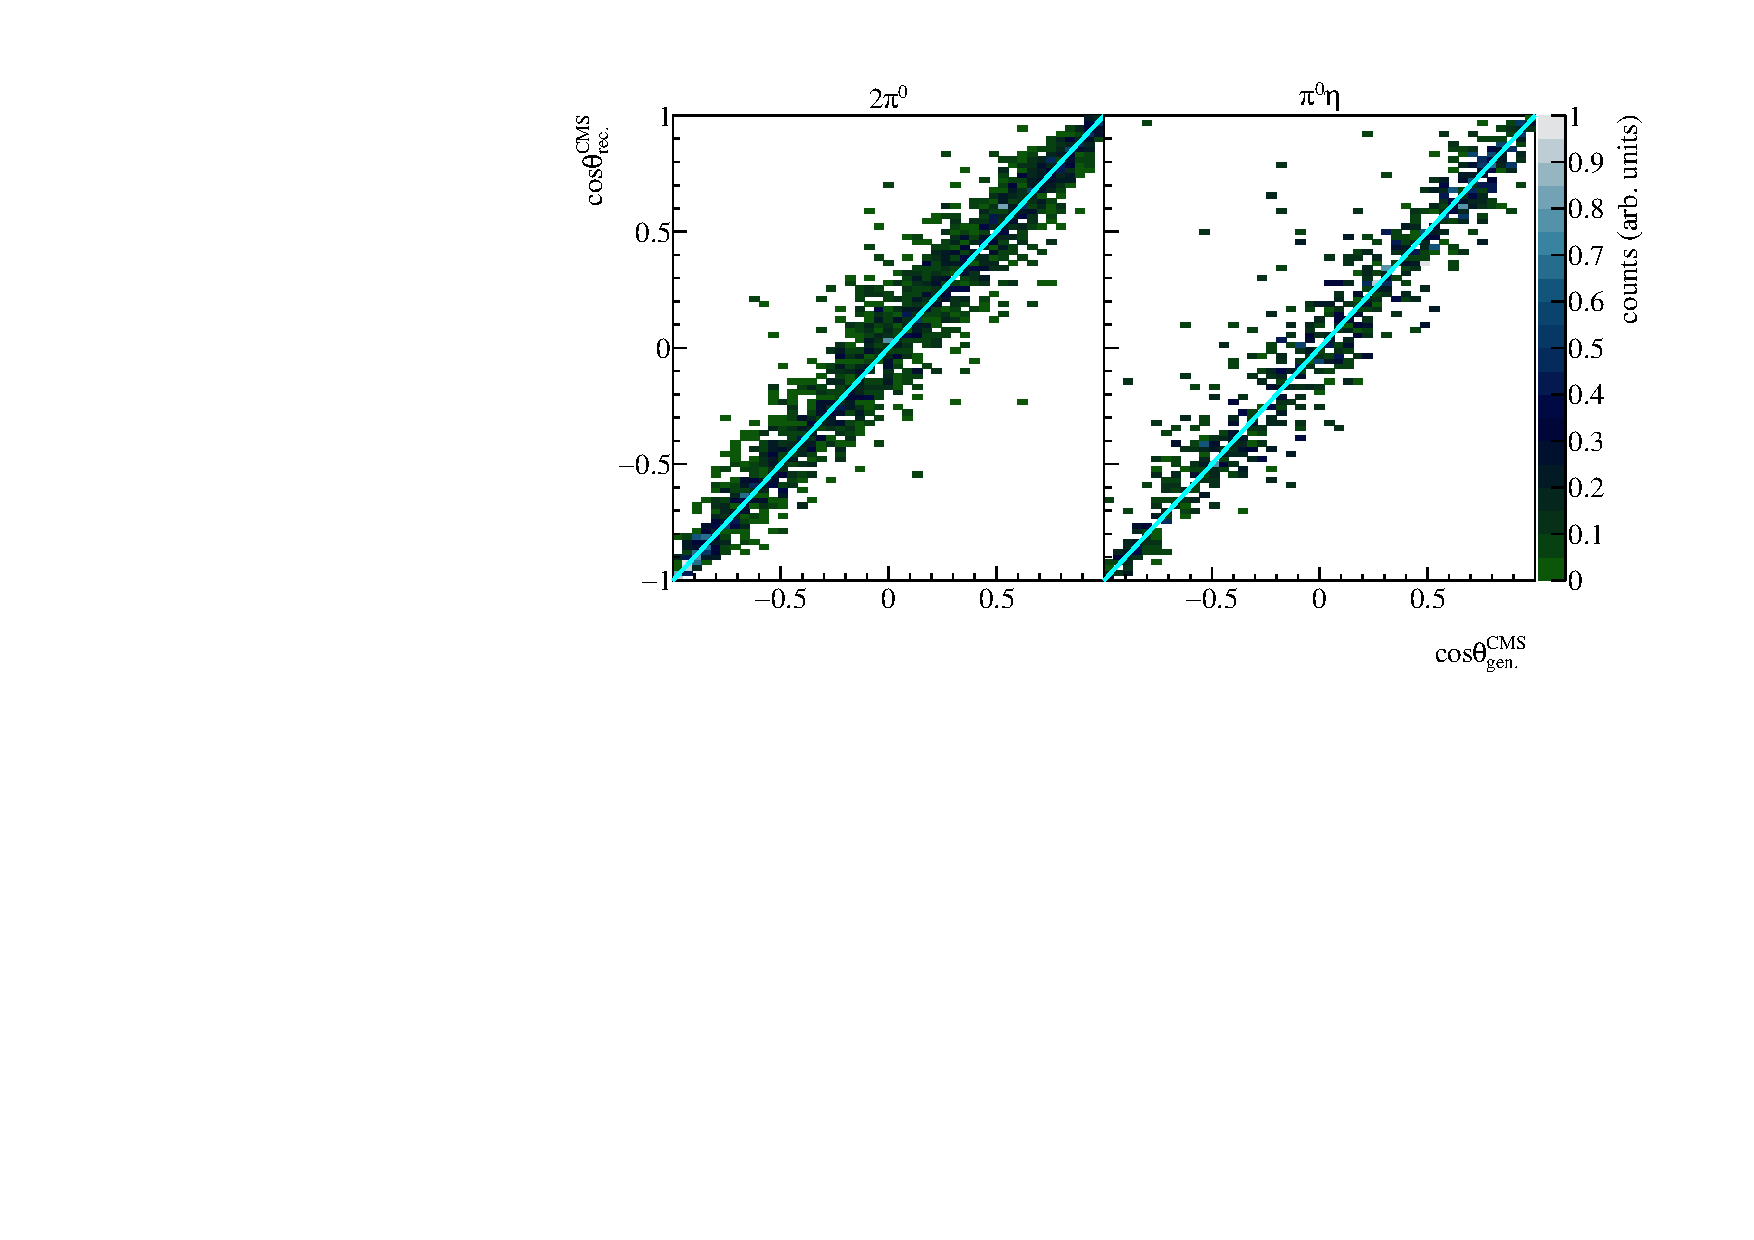
\includegraphics[width=\linewidth]{../figs/hydrogen/mcgammas_ct.pdf}
	\caption{Generated CMS angle $\cos\theta_\text{gen.}$ vs. reconstructed CMS angle $\cos\theta_\text{rec.}$ for both background reactions. The slope $\cos\theta_\text{gen.}=\cos\theta_\text{rec.}$ is indicated by the solid line.}
	\label{fig:mccostheta}
\end{figure}
\subsection{Examination of additional cuts}
\label{subsec:addcuts}
Since the background contributions are significantly beyond a neglible amount it would be desirable to remove them through additional cuts that at the same time do not remove too many signal events. However, this proved to be a complicated task because the background reactions are reconstructed from real photons which happen to be in the $\eta'$ invariant mass range. Therefore they are not distinguishable from $\eta'\to\gamma\gamma$ photons in terms of energy, momentum (direction) or created clustersize in the calorimeter crystals. The combination of two photons into one also is not observable as such since the impact of one photon with energy $E$ may create a cluster with clustersize $C$ which at the same time can be created by two photons in the same direction with energies $E_1+E_2=E$ and clustersizes $C_1+C_2=C$. Thus, to find any characteristics that separate background from signal events, one has to analyze properties of either the recoil proton or the reaction kinematics as a whole.
\subsubsection{Proton cut}
Very close to the $\eta'$ production threshold, the meson system is not boosted very much in forward direction as long as real $\eta'$ mesons are produced. As a consequence the recoil proton may escape to very forward angles in the lab system which corresponds to the proton being detected in the MiniTAPS calorimeter. Falsely reconstructed $2\pi^0$ or $\pi^0\eta$ events have lower production thresholds such that the mesons will be boosted forward and the recoil proton is detected rather in the foward detector or the Crystal Barrel calorimeter. Figure \ref{fig:p_det} shows for the first two energy bins (starting at \SI{1400}{\mega\eV}) the detector that was hit by the recoil proton for $\eta', 2\pi^0$ and $\pi^0\eta$ MC data. At threshold nearly all protons of $\eta'$ events are detected in the MiniTAPS calorimeter while this is only the case for $57\%$ of $2\pi^0$ events and $20\%$ of $\pi^0\eta$ events. Towards higher energies this distribution along detectors smears out and is approximately equal for all reactions. Yet, not enough statistics  are collected in the energy bin close to threshold for a cut based on the proton detector hit to have significance, as this bin contains less than 7\% of total $\eta'$ candidates. The poor statistics in this bin also make determining background from MC fits difficult. Thus, as has been mentioned before, the energy bin from \SIrange{1400}{1500}{\mega\eV} was not included in the analysis. Consequently no cut based on proton detector hits could be applied to the remaining data. Apart from directional information near threshold protons from signal and background events could not be distinguished.
\begin{figure}[htbp]
	\centering
	\begin{subfigure}{\linewidth}
			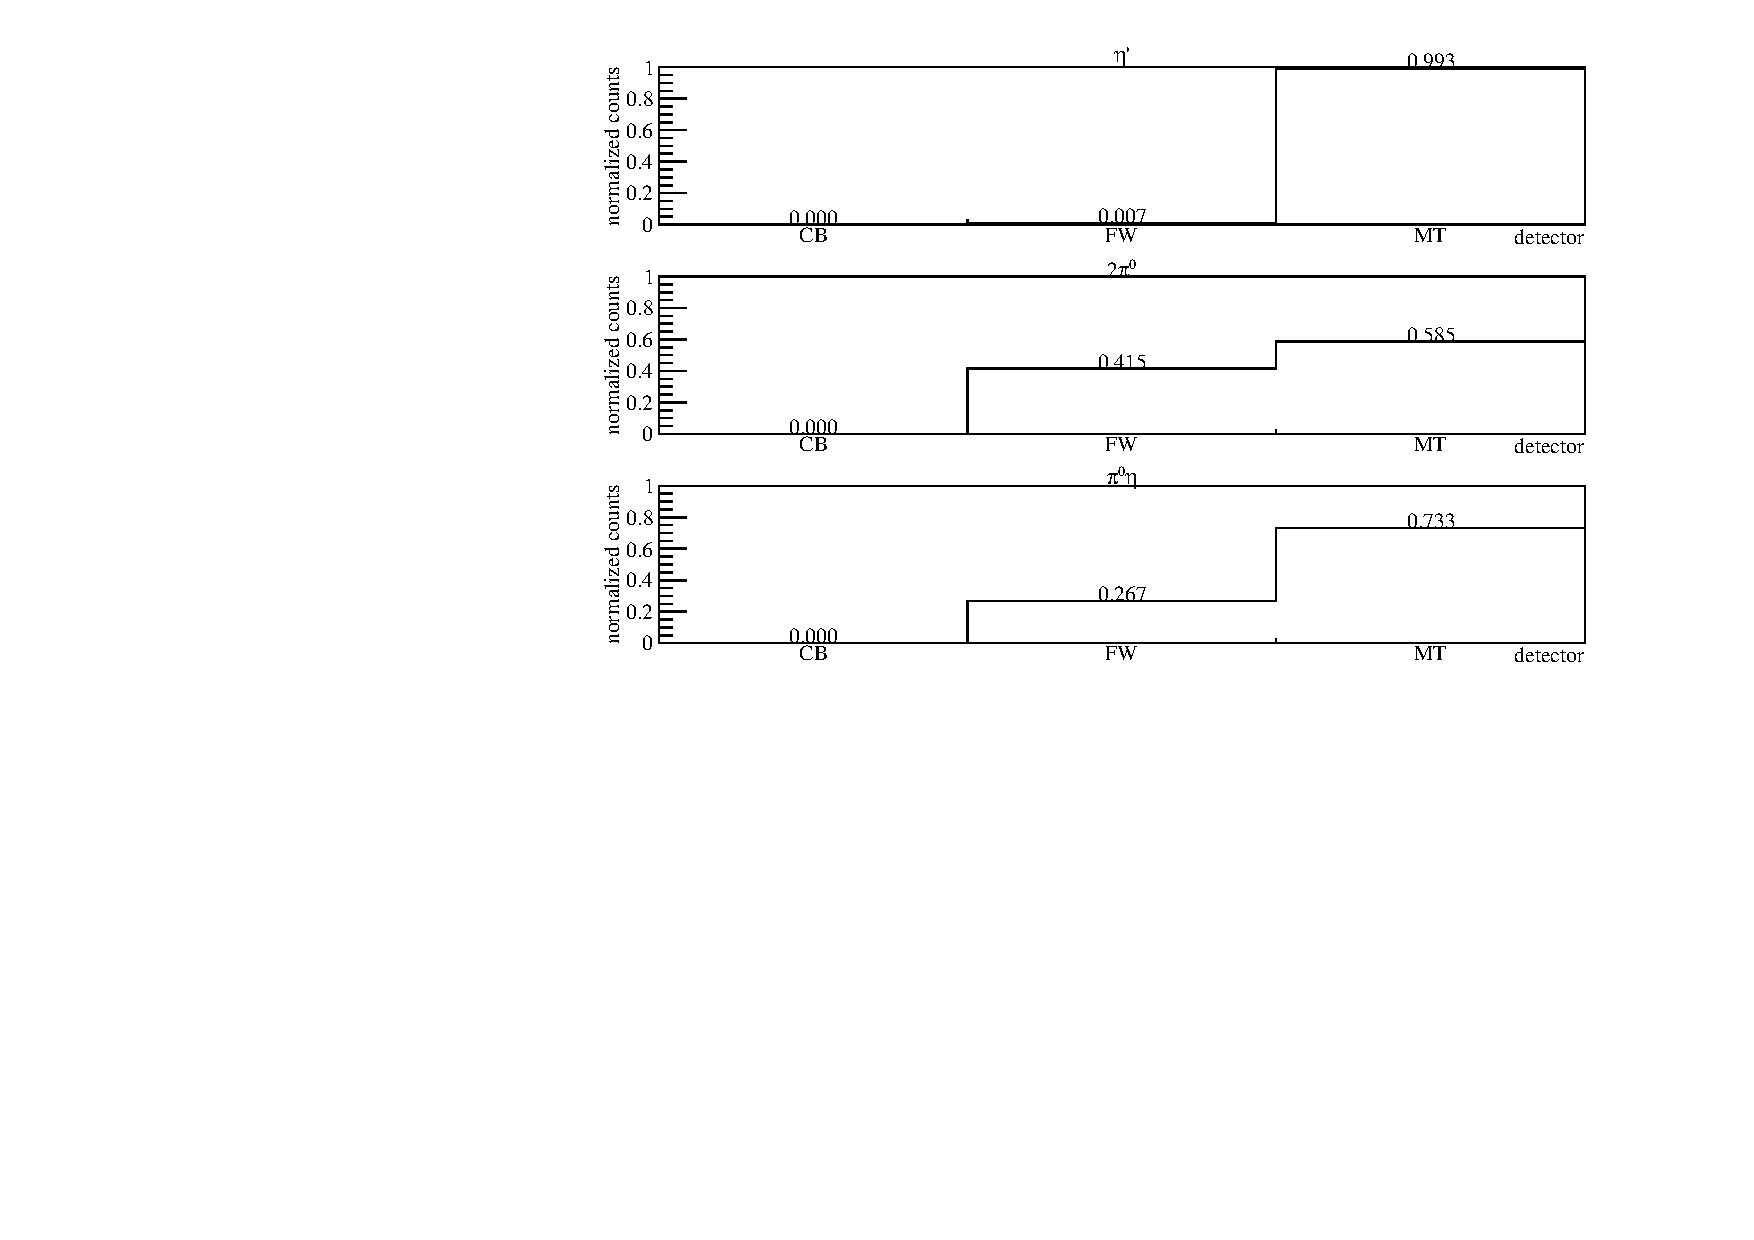
\includegraphics[width=\linewidth]{../figs/hydrogen/p_det/p_det0.pdf}
	 		\subcaption{$\SI{1400}{\mega\eV}\leq E_\gamma<\SI{1500}{\mega\eV}$}
	\end{subfigure}
	\begin{subfigure}{\linewidth}
	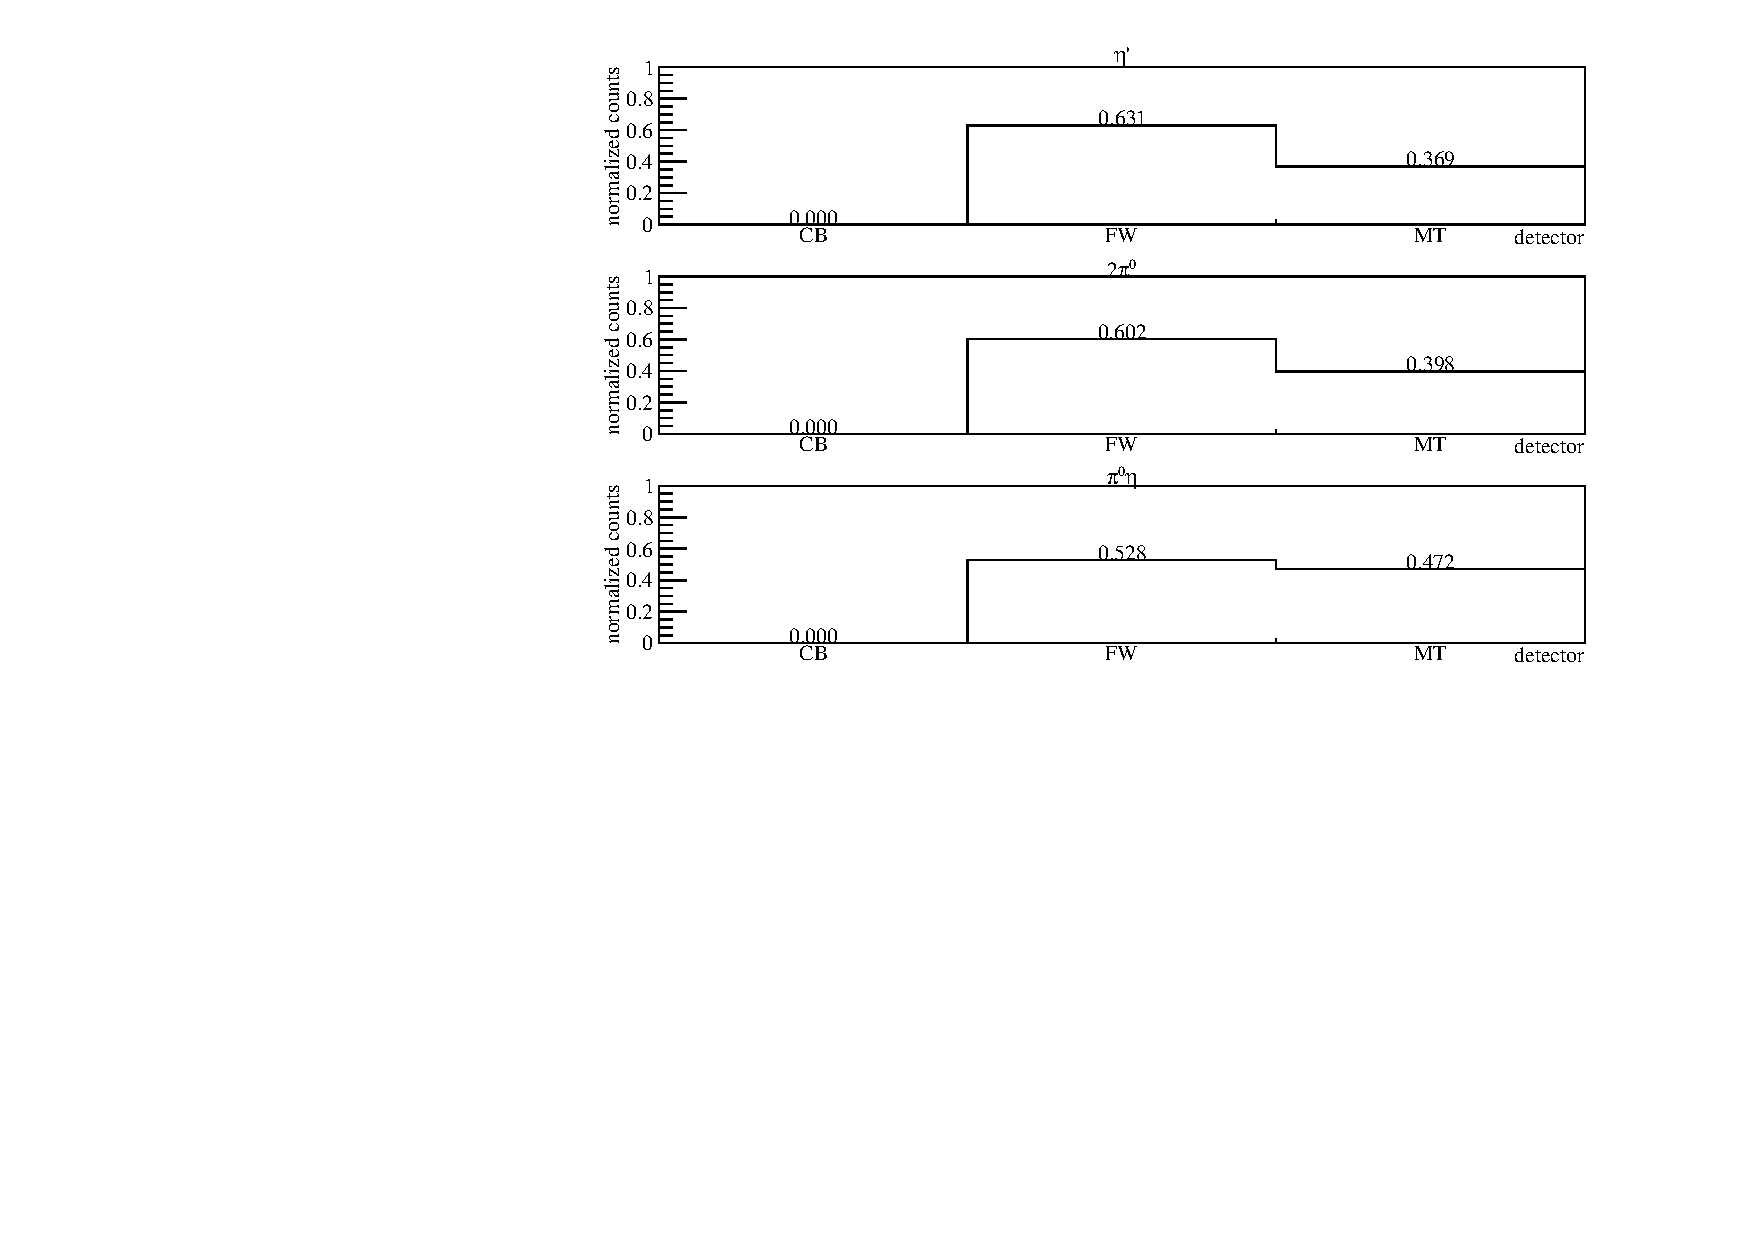
\includegraphics[width=\linewidth]{../figs/hydrogen/p_det/p_det1.pdf}
	\subcaption{$\SI{1500}{\mega\eV}\leq E_\gamma<\SI{1600}{\mega\eV}$}
\end{subfigure}

	\caption{Detector hits of the recoil proton, as obtained from MC data for the production of $\eta',2\pi^0$ and $\pi^0\eta$. CB: Crystal Barrel, FW: forward dector, MT: MiniTAPS}
	\label{fig:p_det}
	
\end{figure}
\subsubsection{Reaction kinematics}
As has been  mentioned before, the measured photoproduction reactions are in fact overdetermined, meaning that one reaction particle can be treated as missing. This can be used to calculate the beam photon energy
\begin{equation}
	E_\gamma^\text{calc}=\frac{-0.5\cdot m_{\eta'}^2+m_pE_{\eta'}}{m_p-E_{\eta}'+|p_z|_{\eta'}},
\label{eq:ebeam}
\end{equation}
where $m_p$ is the proton $m_{\eta'}$ the $\eta'$ mass, $E_{\eta'}$ is the meson energy and $|p_z|_{\eta'}$ is the meson momentum in $z$-direction. Comparing this with the measured beam energy one may tell $\eta'$ events apart from background events where mesons with smaller masses have been produced. If equation \eqref{eq:ebeam} is used to calculate the  beam energy, i.e. inserting the $\eta'$ mass, background events from reactions with smaller masses will cause smaller calculated beam energies. The difference of measured and calculated beam energy $\Delta E= E_\gamma^\text{meas}-E_\gamma^{calc}$ is shown in figure \ref{fig:beame}. The data points are shown as open circles and solid histograms represent fitted MC data where the turquoise histogram is the sum of all MC histograms. A broad peak centred slightly off 0 towards lower energy differences is visible. It also exhibits a broad shoulder towards higher energy differences. The MC describe the data very well, consisting mainly of $\eta'$ and $2\pi^0$ MC, as expected. Yet, the $\pi^0\eta$ MC describe a shape very similar to the $2\pi^0$ MC. The background MC show a trend towards energy differences $>0$, as predicted by equation \eqref{eq:ebeam}. In principle the distribution of background and $\eta'$ MC now allow to introduce an upper bound on the beam energy difference rejecting any desired amount of background. However, simultaneously a significant amount of $\eta'$ events have to be discarded if this cut should have remarkable influence on the background events, as is shown in table \ref{tab:beame}. 
\begin{table}[htbp]
	\centering
	\begin{tabularx}{\linewidth}{ccYY}
		\toprule
		upper limit of $\Delta E$ / MeV& rel. loss of signal events  / \% &\multicolumn{2}{c}{relative loss of bkg. events / \%} \\
		&& $2\pi^0$ & $\pi^0\eta$\\
		\hline
		0 & 36 & 71&59\\
		50 & 21 & 53&36\\
		100& 10&33& 18\\
		150 & 4 & 15 &6\\
		
		\bottomrule
	\end{tabularx}
	\caption{Relative loss in signal and background events if a cut on $\Delta E$ is applied.}
	\label{tab:beame}
\end{table}


Considering that only 8000 $\eta'$ candidates could be extracted, any cut removing sizable fractions of signal events will have grave impact regarding the statistical error for the later analysis of the beam asymmetry. It was decided not to imply any further cuts on the data and proceed with the selected events as described previously. Because results for the beam asymmetry in $2\pi^0$ and $\pi^0\eta$ production are available {\color{red} CITE(P. Mahlberg, Georg Urff?)} it is not crucial to remove all remaining background events since the extracted beam asymmetry can be corrected proportionately, depending on the amount and type of background in a particular bin. 
\begin{figure}[htbp]
	\centering
	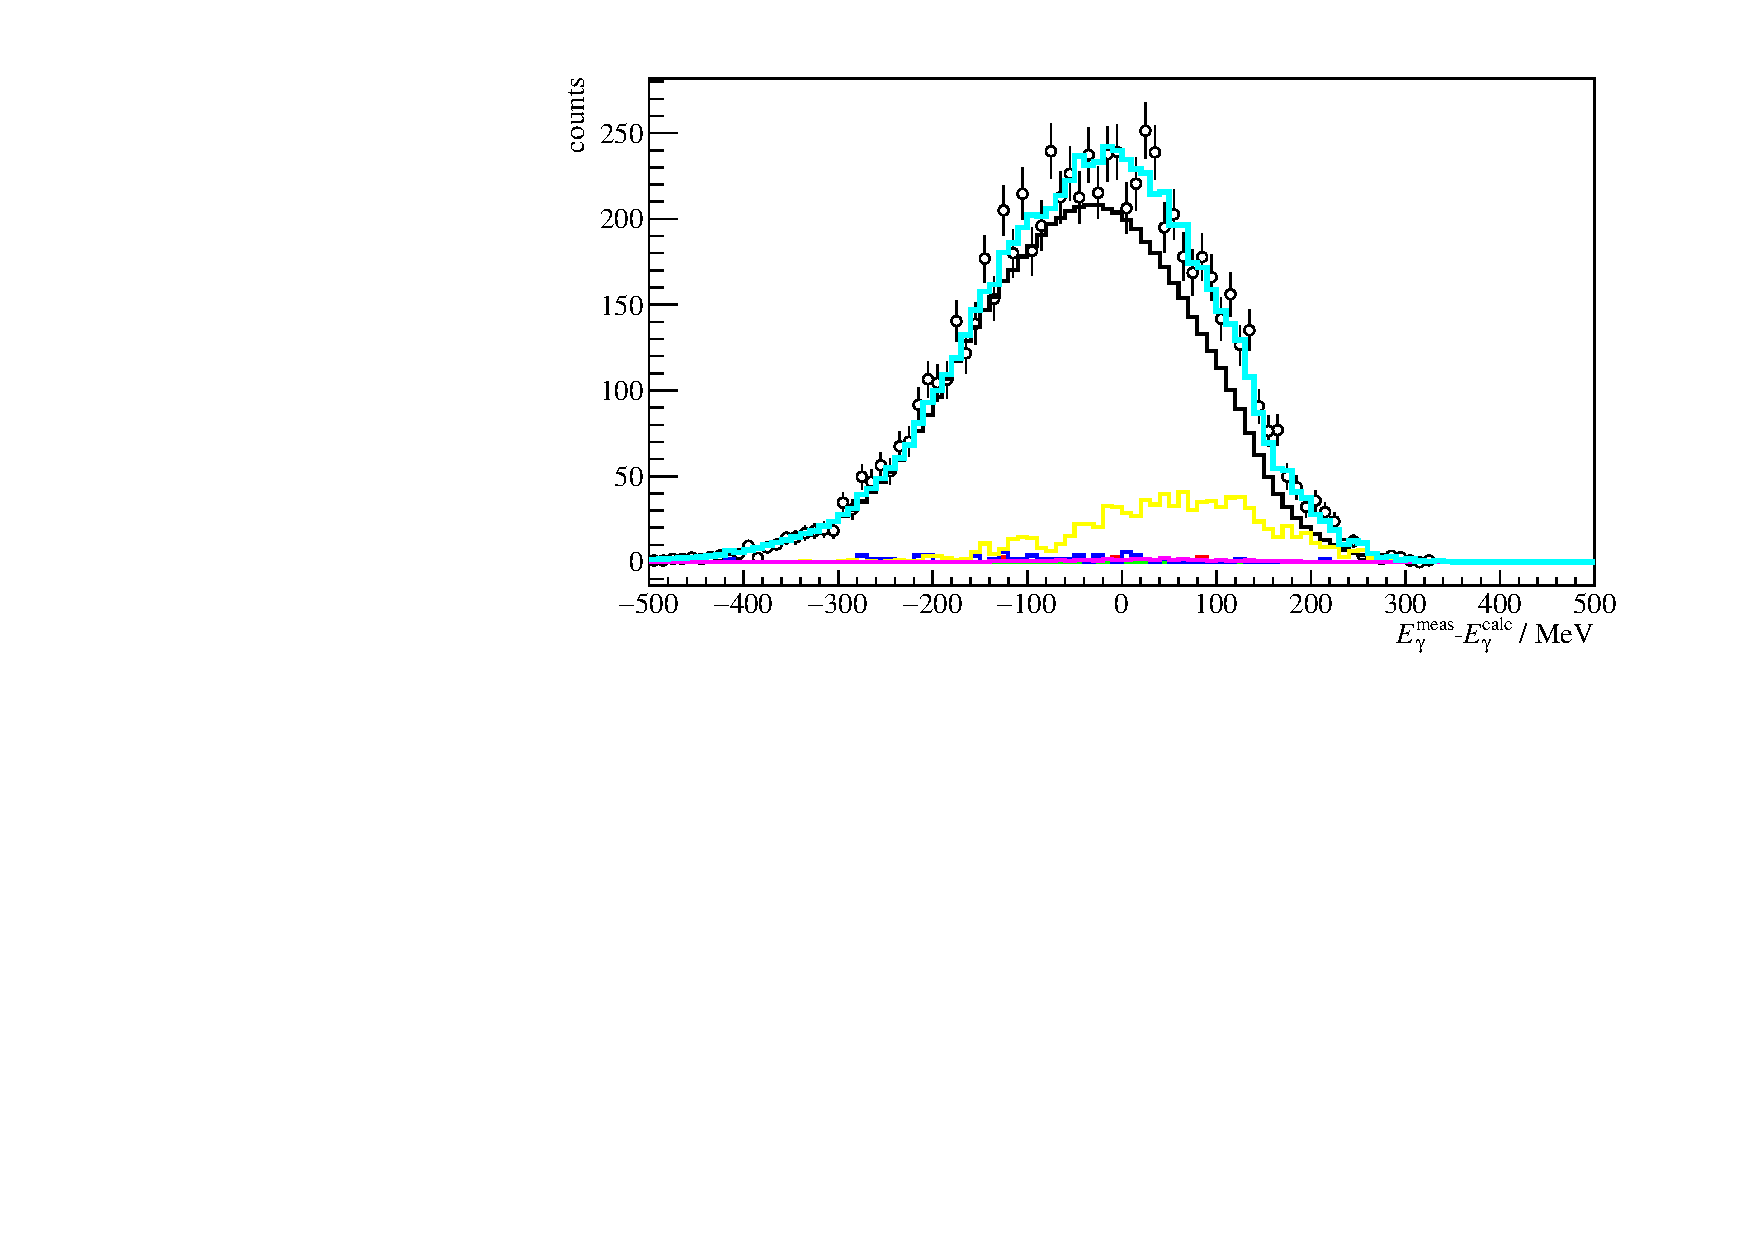
\includegraphics[width=\linewidth]{../figs/hydrogen/calc_beam.pdf}
	\caption{Difference in measured and calculated beam energy. Data points are shown as open circles, MC data as solid histograms: in black $\eta'$, in green $\pi^0$, in red $\eta$, in blue $\omega$, in yellow $2\pi^0$ and in magenta $\pi^0\eta$. The turquoise histogram is the sum of all MC histograms.}
	\label{fig:beame}
\end{figure}

\section{Summary of event selection}
The reaction $\gamma p\to p\eta'$ could be selected successfully. Combinatorical background was removed using the time information of initial and final state particles. Furthermore, the measured energies and momenta of all final state particles were utilized when applying constraints, that were derived from energy and momentum conservation, to $\gamma p\to\eta'\to\gamma\gamma$ event candidates. A significant amount of background still passes the event selection process which could be traced back to $2\pi^0$ and $\pi^0\eta$ production using Monte Carlo simulations. Very restricted possibilities to exclusively select signal from background events were found but in the end not used as they still remove sizable fractions of signal events in order to get rid of background events.

To illustrate again the impact of all applied cuts, the invariant mass summed over all angular and energy bins of the final state photons is shown again in figure \ref{fig:invm_pretty} where the spectrum can be seen after each individual cut successively. While at first only slight structures in the invariant mass spectrum can be observed, in the end a clear, peak-like structure is visible, indicating the general success of the event selection that has been described in this chapter. The signal to background ratio is improved by each applied cut where the time cut clearly removes the most (combinatorical) background. Note that there are differences of three and two orders of magnitude in statistics for $\pi^0$ or $\eta$ meson production compared to $\eta'$ production in the neutral decay channel. 
\begin{figure}[t]
	\centering
	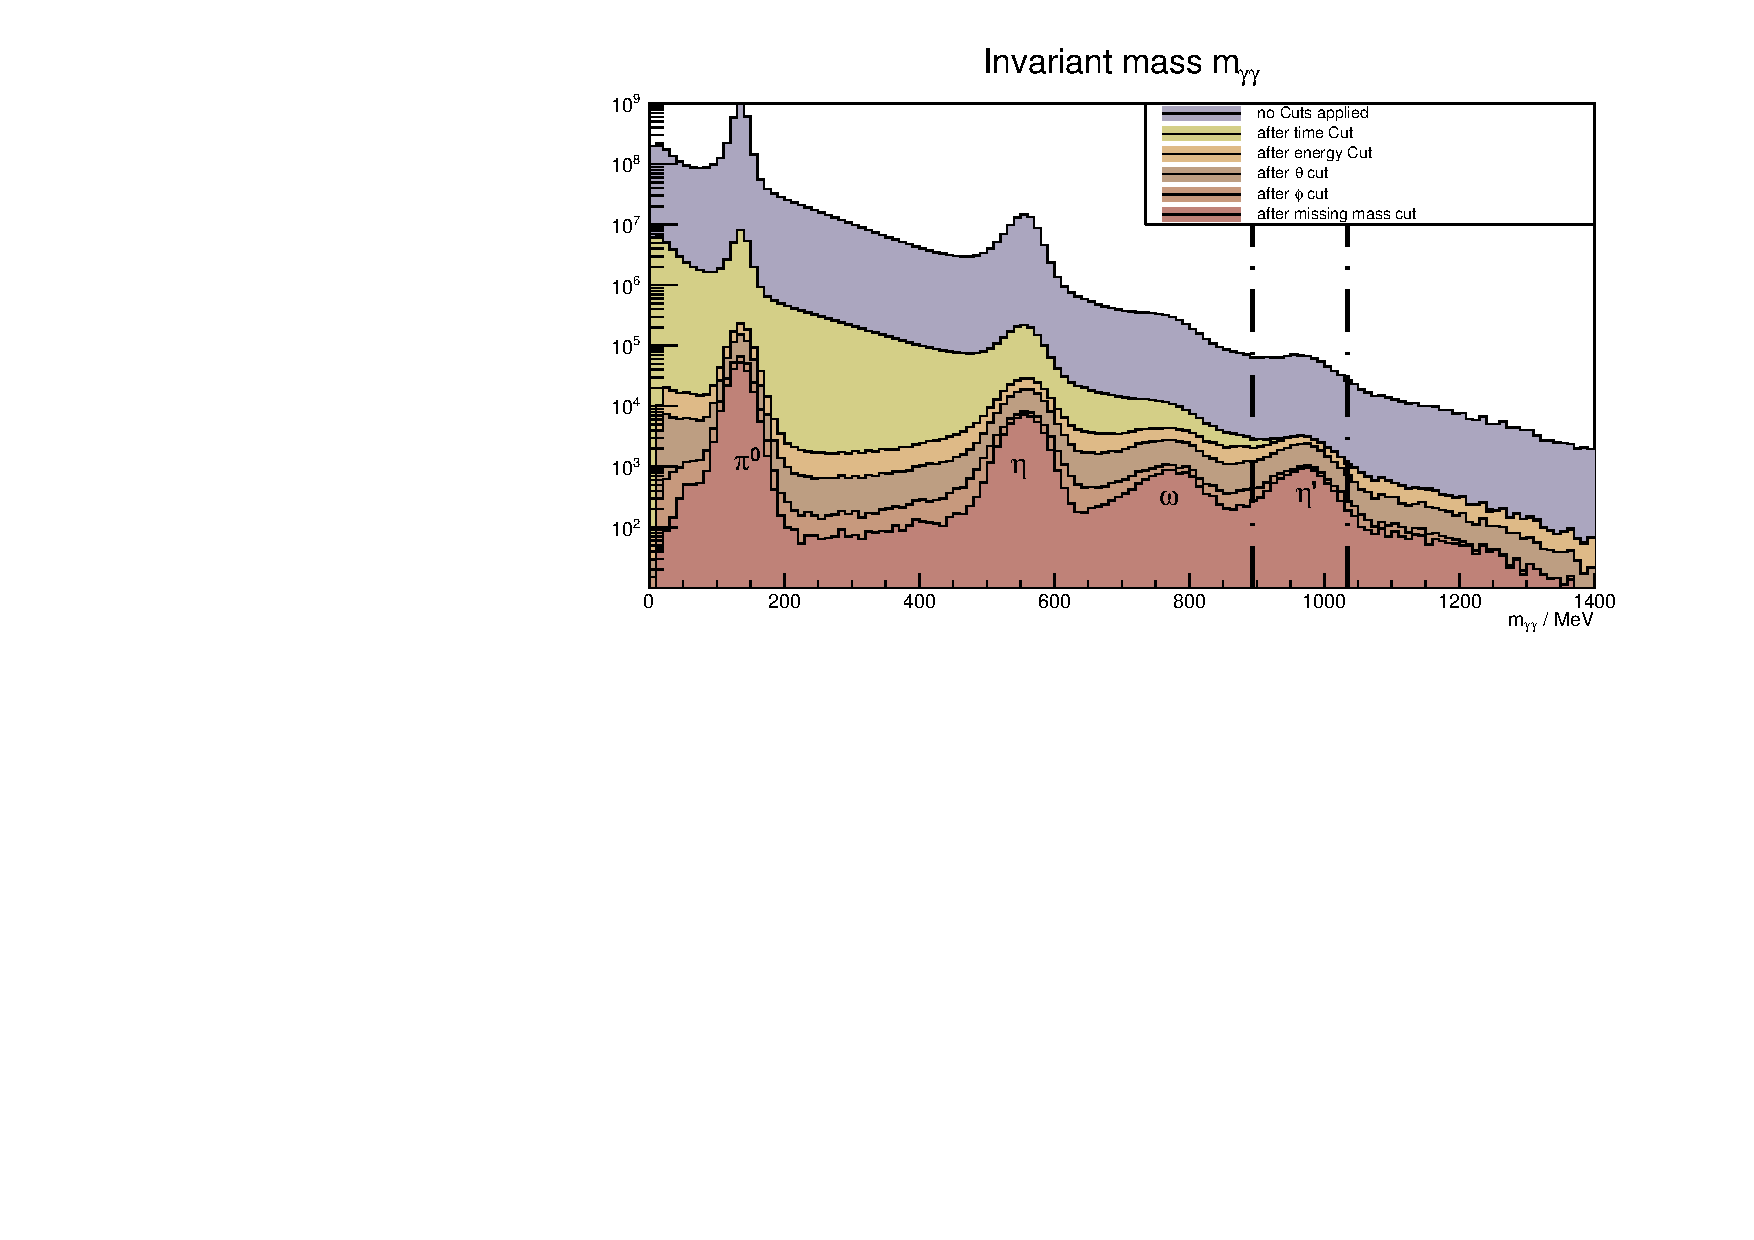
\includegraphics[width=\linewidth]{../figs/hydrogen/inv_mass_pretty.pdf}
	\caption{Invariant mass spectrum passing different stages in the event selection process. In the end clear peaks for all possibly produced mesons are visible. The vertical lines indicate the mean cut ranges over all energy and angle bins.}
	\label{fig:invm_pretty}
\end{figure}

% !TEX root = master_thesis.tex
\chapter{Extraction of the beam asymmetries $\Sigma_{\eta}$ and $\Sigma_{\eta'}$}
The beam asymmetry $\Sigma$ is observable when a linearly polarized photon beam and unpolarized liquid hydrogen target are employed. The polarized cross section $\frac{\text{d}\sigma}{\text{d}\Omega}_\text{pol}$ is not symmetric in the azimuthal angle $\phi$ anymore as opposed to the unpolarized cross section $\frac{\text{d}\sigma}{\text{d}\Omega}_0$. It is rather modulated by a cosine dependence which scales with the polarization observable $\Sigma$ and the (linear) beam polarization $p_\gamma$, see equation \eqref{eq:asym} \cite{san}.
\begin{equation}
	\frac{\text{d}\sigma}{\text{d}\Omega}_\text{pol}\left(E_\gamma,\cos\theta,\phi\right)=\frac{\text{d}\sigma}{\text{d}\Omega}_0\left(E_\gamma,\cos\theta\right)\cdot\left[1-p_\gamma\Sigma\left(E_\gamma,\cos\theta\right)\cos\left(2\varphi\right)\right]
	\label{eq:asym}
\end{equation}
Since the incident photon beam is polarized, photon momentum $\vec{k}$ and polarization $\vec{\epsilon}$ span a plane which is referred to as the beam polarization plane. This plane is tilted by the angle $\varphi$ with respect to the reaction plane which is defined by the final state momenta. Naturally, this plane builds the angle $\phi$ in the laboratory system. At the same time the angle of the beam polarization plane in the same reference frame is defined as $\alpha$. It holds 
\begin{equation}
	\varphi=\alpha-\phi.
\end{equation} Figure \ref{fig:angles} illustrates definitions of all angles and planes. 
 \begin{figure}[htbp]
	\centering
	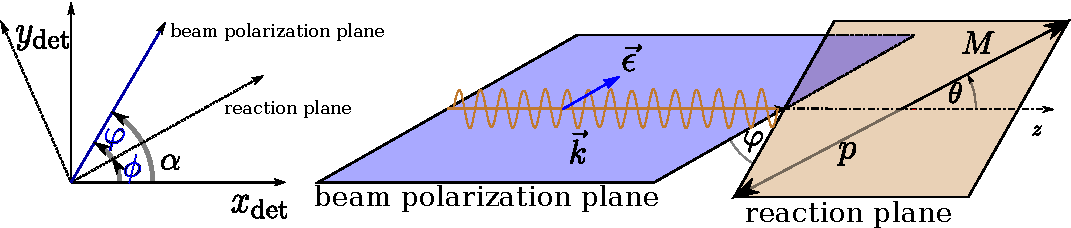
\includegraphics[width=\linewidth]{../DPG2022/figs/angles.pdf}
	\caption{Left: Definition of angles $\alpha,\phi,\varphi$. Right: Photon momentum $\vec{k}$ and polarization  $\vec{\epsilon}$ define the beam polarization plane while the reaction plane is defined by the recoil proton $p$ and produced meson $M$.}
	\label{fig:angles}
\end{figure} 
Theoretically the beam asymmetry can be determined by a measurement of the cross section and a fit using equation \eqref{eq:asym}. However, when calculating polarized cross sections, it is important to have good control over flux normalization and detector acceptance in three dimensions $(E_\gamma,\cos\theta,\phi)$. To avoid this, the measurement of asymmetries can be used to access the polarization observable $\Sigma$ instead. Particularly, data is taken for two distinct orthogonal polarization settings corresponding to $\alpha=\pm\SI{45}{\degree}$.

This chapter will illustrate the process of determining the beam asymmetry for $\eta$ and $\eta'$ photoproduction. The published results of $\Sigma_{\eta}$ \cite{farahphd,eta} are used to check the accuracy and functionality of employed bayesian methods. Bayesian methods, as well as traditional frequentist approaches are used afterwards to extract new results for $\Sigma_{\eta'}$. First, the determination of the beam photon polarization is briefly described, then the used methods will be presented and subsequently their application for each final state, respectively.
\section{Methods}
\label{sec:meth}
The beam asymmetry has to be determined via fits to $\phi$ distributions obtained from data. These are performed as either binned or unbinned fits. Both methods allow the application of Bayesian methods as will be discussed in the following. Additionally the advantages and disadvantages off all methods are compared.
\subsection{Event yield asymmetries}
Measurements were made in two distinct polarization settings $\alpha=\pm\SI{45}{\degree}=\alpha^{\bot/\parallel}$. Thus, the polarized cross sections for both settings are given by\footnote{The dependencies of polarized and unpolarized cross sections as well as the beam asymmetry like in equation \eqref{eq:asym} are implied}
\begin{equation}
	\frac{\text{d}\sigma}{\text{d}\Omega}_\text{pol}^\parallel=\frac{\text{d}\sigma}{\text{d}\Omega}_0\cdot\left[1-p_\gamma^\parallel\Sigma\cos\left(2\left(\alpha^\parallel-\phi\right)\right)\right]
	\label{eq:polcs0}
\end{equation}
and 
\begin{align}
	\frac{\text{d}\sigma}{\text{d}\Omega}_\text{pol}^\bot&=\frac{\text{d}\sigma}{\text{d}\Omega}_0\cdot\left[1-p_\gamma^\bot\Sigma\cos\left(2\left(\alpha^\bot-\phi\right)\right)\right]\label{eq:polcs00}\\
	&=\frac{\text{d}\sigma}{\text{d}\Omega}_0\cdot\left[1+p_\gamma^\bot\Sigma\cos\left(2\left(\alpha^\parallel-\phi\right)\right)\right].\label{eq:polcs}
\end{align}
Note that equation \eqref{eq:polcs} holds, because 
\begin{align*}
	\alpha^\bot=\alpha^\parallel+\pi/2 &&\text{and}&&\cos x = -1\cdot\cos(x+\pi).
\end{align*}
Consider now taking the difference of equations \eqref{eq:polcs0} and \eqref{eq:polcs}
\begin{equation}
	\frac{\text{d}\sigma}{\text{d}\Omega}_\text{pol}^\bot-\frac{\text{d}\sigma}{\text{d}\Omega}_\text{pol}^\parallel=\frac{\text{d}\sigma}{\text{d}\Omega}_0\cdot\left(p_\gamma^\bot+p_\gamma^\parallel\right)\Sigma\cos\left(2\left(\alpha^\parallel-\phi\right)\right).
\end{equation}
One can further eliminate the unpolarized cross section from this equation by dividing by the polarization weighted sum of equations \eqref{eq:polcs0} and \eqref{eq:polcs}
\begin{equation}
	\alpha\cdot\frac{\text{d}\sigma}{\text{d}\Omega}_\text{pol}^\bot+\beta\cdot\frac{\text{d}\sigma}{\text{d}\Omega}_\text{pol}^\parallel=\frac{\text{d}\sigma}{\text{d}\Omega}_0\cdot\left[\alpha+\beta-\left(\alpha p_\gamma^\bot-\beta p_\gamma^\parallel\right)\Sigma\cos\left(2\left(\alpha^\parallel-\phi\right)\right)\right]\overset{!}{=}2\frac{\text{d}\sigma}{\text{d}\Omega}_0.
\end{equation}
Since $$\frac{\text{d}}{\text{d}\phi}\frac{\text{d}\sigma}{\text{d}\Omega}_0\overset{!}{=}0\forall\phi,$$ it holds \begin{align}
	\alpha p_\gamma^\parallel-\beta p_\gamma^\bot \overset{!}{=}0 && \alpha+\beta\overset{!}{=}2,
\end{align}
such that
\begin{align}
	\alpha =\frac{2p_\gamma^\parallel}{p_\gamma^\bot+p_\gamma^\parallel} && \beta=\frac{2p_\gamma^\bot}{p_\gamma^\bot+p_\gamma^\parallel}.
	\label{eq:alphabeta}
\end{align}
The beam asymmetry $\Sigma$ is thus accessible via the asymmetry \begin{equation}
	A(\phi)=\frac{\frac{\text{d}\sigma}{\text{d}\Omega}_\text{pol}^\bot-\frac{\text{d}\sigma}{\text{d}\Omega}_\text{pol}^\parallel}{p_\gamma^\parallel\frac{\text{d}\sigma}{\text{d}\Omega}_\text{pol}^\bot+p_\gamma^\bot\frac{\text{d}\sigma}{\text{d}\Omega}_\text{pol}^\parallel}=\Sigma\cos\left(2\left(\alpha^\parallel-\phi\right)\right).
	\label{eq:asymfit}
\end{equation}
At this point one can now make use of the fact that in any scattering reaction the number of events $N$ is given by the product of luminosity $L$ and total cross section $\sigma$ $$N=L\cdot\sigma=\Phi\cdot N_t\cdot\frac{\text{d}\sigma}{\text{d}\Omega}\cdot\Delta\Omega,$$
where $\Phi$ is the beam flux, $N_t$ the number of target particles and $\Delta\Omega$ is the solid angle covered by the detector. Substituting this in equation \eqref{eq:asymfit} one can build the asymmetry $A(\phi)$ using only the (flux-)normalized event yields $\tilde{N}^{\parallel/\bot}\left(E_\gamma,\cos\theta,\phi\right)$\footnote{again, arguments $\left(E_\gamma,\cos\theta,\phi\right)$ are implied.}
\begin{equation}
	A(\phi)=\frac{\tilde{N}^\bot-\tilde{N}^\parallel}{p_\gamma^\parallel\tilde{N}^\bot+p_\gamma^\bot\tilde{N}^\parallel}=\Sigma\cos\left(2\left(\alpha^\parallel-\phi\right)\right).
	\label{eq:evyieldasym}
\end{equation}
Alternatively, the event yields $N$ can also be normalized by integrating over the total azimuthal angle range in each bin of $(E_\gamma,\cos\theta)$. This normalization technique has been used in reference \cite{farahphd} and will also be used in this work. Using appropriate binning in $\phi$ in addition to beam energy and meson polar angle the asymmetry can be build for all kinematic bins and the beam asymmetry then be extracted via a one-Parameter fit. The statistical errors for $A(\phi)$ are given by \textsc{Gaussian} error propagation (see appendix \ref{sec:stat_err}). 
\subsubsection{Frequentist}
The beam asymmetry can now be determined via a frequentist fit, where $\Sigma$ is determined such that the $\chi^2$ value resulting from the data points and equation \ref{eq:evyieldasym} is minimized. The results are point estimates with statistical error bars that are also obtained from the fit: $\hat{\Sigma}\pm\sigma_{\hat{\Sigma}}$. In addition $\chi^2/\text{NDF}\approx1$ may be verified in order to diagnose the fit itself. Multiple automated minimization and calculation algorithms for $\chi^2$ fitting are available as open source. The \emph{Python} \cite{python} module \emph{scipy} \cite{scipy} and \emph{ROOT} \cite{root} offer e.g. the methods \texttt{scipy.optimize.curve\_fit} \cite{pFit} and \texttt{TH1::Fit()} \cite{rFit} for discrete/binned data, which were used in the analysis.
\subsubsection{\textsc{Bayesian}}
Following section \ref{sec:bayes}, where the basics of \textsc{Bayesian} inference were discussed, the goal of a \textsc{Bayesian} approach is to sample marginal posterior distributions for each fitted parameter from the joint posterior $p(\boldsymbol{\theta}|y)$ which depends on the observed data $y$. The joint posterior itself is proportional to the product of priors $\pi(\boldsymbol{\theta})$ and likelihood $\mathcal{L}(y|\boldsymbol{\theta})$ (\textsc{Bayes'} theorem). This collapses to a one parameter problem in the case of fitting the event yield asymmetries (Eq. \eqref{eq:evyieldasym})
\begin{equation}
	p(\Sigma|y)\propto \pi({\Sigma})\cdot \mathcal{L}(y|\Sigma).
\end{equation}
However, to be able to sample from a joint posterior, prior and likelihood need to be specified. In order not to bias the fit towards any particular values, the prior is chosen non-informative, realized by a broad \textsc{Gaussian} centered at 0 which is truncated to the physically allowed parameter space of $\Sigma\in[-1,1]$. Furthermore, the likelihood is formulated assuming \textsc{Gaussian} errors $\epsilon_n$ at each data point $y_n$, which should be described by the asymmetry (Eq \eqref{eq:evyieldasym}) at bin $n$ $A(\phi_n;\Sigma)$, i. e. \footnote{Remember the notation introduced in section \ref{sec:bayes}: $x\sim\mathcal{N}(\mu,\sigma)=\mathcal{N}(x|\mu,\sigma)=\frac{1}{\sqrt{2\pi\sigma^2}}e^{-\frac{(x-\mu)^2}{2\sigma^2}}$}
\begin{align}
	\Sigma \sim \mathcal{N}\left(0,1\right)_{[-1,1]} && y_n=A\left(\phi_n;\Sigma\right)+\epsilon_n && \epsilon_n\sim\mathcal{N}\left(0,\sigma_n\right),
\end{align}
which is equivalent to
\begin{align}
	 \Sigma \sim \mathcal{N}(0,1) &&y_n\sim\mathcal{N}\left(A(\phi_n;\Sigma),\sigma_n\right).
\end{align}
The likelihood of all data points now evaluates to the product of the likelihood at each data point $y_n$ and the posterior results in \begin{align}
	p(\Sigma|y)&\propto\pi(\Sigma)\cdot\mathcal{L}(y|\Sigma)=\mathcal{N}\left(\Sigma|0,1\right)_{[-1,1]}\cdot\prod_{n}\mathcal{N}\left(y_n|A\left(\phi_n;\Sigma\right),\sigma_n\right)\\
	\Leftrightarrow -\ln p(\Sigma|y)&=\frac{1}{2}\Sigma^2+\frac{1}{2}\sum_{n}\left(\frac{y_n-A\left(\phi_n;\Sigma\right)}{\sigma_n}\right)^2+\text{ constant terms }, 
\end{align}
such that all ingredients are present to form a fully \textsc{Bayesian} probabilistic model\footnote{Note that the sampling aims only to reflect the right proportionality of the (marginal) posterior. Thus, constant terms can be dropped and are of no further interest \cite{stan}.}. This model was implemented in Stan \cite{stan}, directly giving access to samples from the posterior obtained with the No-U-Turn-Sampler (NUTS) \cite{stan,nuts}. Hereby, the sampling is restricted to the allowed parameter region $\Sigma\in[-1,1]$. As a measure of goodness of fit, the $p$-values obtained from the posterior predictive distributions, as introduced in section \ref{sec:bayes}, are reviewed. To diagnose the convergence of the MCMC fit, sensible values for $\hat{R}$ and the Monte-Carlo standard error $\sigma_\text{MCSE}$ are verified.
\subsection{Event based fit}
Although intuitive and easily implementable the binned fit --\textsc{Bayesian} or not-- has one critical disadvantage: it is inevitable that information is lost because the asymmetry $A(\phi)$ is a binned quantity and hence, the choice of binning influences the fit results. This is discussed in more detail in appendix \ref{app:binnedfits}. Especially kinematic bins with low statistics show this behavior. To circumvent this problem, an \emph{unbinned fit}, based on the likelihood function for each event, can be performed. Also, no assumptions on the distribution of statistical errors have to be made since each event is taken into account individually. Yet, the event based fit does not provide any measure of goodness of fit, so that the study of toy Monte Carlo data is essential when checking the working principle of the method.

In a polarized experiment the azimuthal angle distribution of events is not isotropic, but modulated by a cosine term coupling to beam asymmetry $\Sigma$ and beam polarization $p_\gamma^{\parallel/\bot}$ for each setting $\alpha^{\parallel/\bot}$, as is expressed through the respective differential cross sections in Equations \ref{eq:polcs0} and \ref{eq:polcs00}. Since the number of events is proportional to the cross section, the probability $p\left(\phi,p_\gamma^{\parallel/\bot}\big|\Sigma\right)$ to find an event under the azimuthal angle $\phi$ for a given bin of $\left(E_\gamma,\cos\theta\right)$ and setting $\alpha^{\parallel/\bot}$ is \footnote{Note: Normalizing $p\left(\phi,p_\gamma^{\parallel/\bot}\big|\Sigma\right)$ to $2\pi$ (or any other arbitrary constant) is sufficient for the fit as long as the integral does not depend on the fit parameters. The normalization to $2\pi$ is chosen for better readability. However, to calculate actual probabilities, one must multiply Eq. \eqref{eq:prob0} by $2\pi$.} \begin{equation}
	p\left(\phi,p_\gamma^{\parallel/\bot}\big|\Sigma\right)=\frac{\left[1\mp p_\gamma^{\parallel/\bot}\Sigma\cos\left(2\left(\alpha^\parallel-\phi\right)\right)\right]}{\frac{1}{2\pi}\int_{0}^{2\pi}\text{d}\phi\left[1\mp p_\gamma^{\parallel/\bot}\Sigma\cos\left(2\left(\alpha^\parallel-\phi\right)\right)\right] }.
	\label{eq:prob0}
\end{equation}
This is only true for an idealized experiment with acceptance $\epsilon=\text{const}\forall\phi$, so that the acceptance $\epsilon(\phi)$ has to be included in the probability for each event. As demonstrated in reference \cite{hartmannphd} a \textsc{Fourier} series truncated after the fourth order is sufficient to model any occurring function $$\epsilon\left(\phi\right)=\sum_{k=0}^4a_k\sin\left( k\phi\right)+b_k\cos\left(k\phi\right),$$ where the eight detector coefficients $a_k$ and $b_k$ are determined from the fit. With this the measurable probability $\tilde{p}\left(\phi,p_\gamma^{\parallel/\bot}\big|\Sigma,a,b\right)$ is 
\begin{align}
	\tilde{p}\left(\phi,p_\gamma^{\parallel/\bot}\big|\Sigma,a,b\right)&\propto\left[1\mp p_\gamma^{\parallel/\bot}\Sigma\cos\left(2\left(\alpha^\parallel-\phi\right)\right)\right]\cdot\epsilon(\phi)\\&=\left[1\mp p_\gamma^{\parallel/\bot}\Sigma\cos\left(2\left(\alpha^\parallel-\phi\right)\right)\right]\cdot\left(\sum_{k=0}^4a_k\sin\left( k\phi\right)+b_k\cos\left(k\phi\right)\right),
\end{align}
where $a:=\{a_k\}_{k=0}^4, b:=\{b_k\}_{k=0}^4$. Finally, normalizing $\frac{1}{2\pi}\int_{0}^{2\pi}\text{d}\phi\tilde{p}\left(\phi,p_\gamma^{\parallel/\bot}\big|\Sigma,a,b\right)\overset{!}{=}1$,
\begin{equation}
	\tilde{p}\left(\phi,p_\gamma^{\parallel/\bot}\big|\Sigma,a,b\right)=\frac{\left[1\mp p_\gamma^{\parallel/\bot}\Sigma\cos\left(2\left(\alpha^\parallel-\phi\right)\right)\right]\cdot\left(\sum_{k=0}^4a_k\sin\left( k\phi\right)+b_k\cos\left(k\phi\right)\right)}{1\pm\frac{1}{2}a_2p_\gamma^{\parallel/\bot}\Sigma}.
	\label{eq:prob}
\end{equation}
The respective polarization setting $\alpha^{\parallel/\bot}$ determines the sign in the normalizing constant which allows an uncorrelated estimation of the detector coefficient $a_2$ and the beam asymmetry $\Sigma$. To simplify notation and implementation, Equation \eqref{eq:prob} can be written as \emph{one} probability for all events -- irregardless of polarization setting -- if the polarization values $p_\gamma^\parallel$ are multiplied by $(-1)$ and summarized as $p_\gamma$: \begin{equation}
	\tilde{p}\left(\phi,p_\gamma\big|\Sigma,a,b\right)=\frac{\left[1+p_\gamma\Sigma\cos\left(2\left(\alpha-\phi\right)\right)\right]\cdot\left(\sum_{k=0}^4a_k\sin\left( k\phi\right)+b_k\cos\left(k\phi\right)\right)}{1-\frac{1}{2}a_2p_\gamma\Sigma},
	\label{eq:prob}
\end{equation} 
with $\alpha=\SI{-45}{\degree}$ fixed.

In section \ref{sec:time} the subtraction of uncorrelated time background was discussed via a sideband subtraction. Naturally, without binning the data, this strategy is invalid and prompt peak and sideband events have to be fitted simultaneously. Hereby it is important to consider that the random time background is realized as flat distribution underneath the complete reaction time spectrum (cf. Figure \ref{fig:time_r}), \emph{including} the range of the prompt peak. The fraction of true coincident events to random coincidences is given as \begin{equation}
	f=\frac{N_\text{prompt}-w\cdot N_\text{sideband}}{N_\text{prompt}},
\end{equation}
where $N_\text{prompt}$ and $N_\text{sideband}$ are the number of events where the reaction time lies within the prompt peak or sideband, respectively. $w$ is the ratio of the widths of the chosen prompt peak and sideband
ranges, see section \ref{sec:time}. It is now assumed that the random coincidences will exhibit an asymmetry $\Sigma^\text{bkg}$ of their own and are not necessarily described by the detector coefficients $a$ and $b$ but rather by $a^\text{bkg}$ and $b^\text{bkg}$. The probability to detect a prompt peak event $p_\text{prompt}$ and the probability to measure a sideband event $p_\text{sideband}$ are then given by 
\begin{align}
p_\text{prompt}\left(\phi,p_\gamma,\big|\Sigma,a,b,\Sigma^\text{bkg},a^\text{bkg},b^\text{bkg}\right)&=f\cdot\tilde{p}\left(\phi,p_\gamma\big|\Sigma,a,b\right)+\left(1-f\right)\cdot\tilde{p}\left(\phi,p_\gamma\big|\Sigma^\text{bkg},a^\text{bkg},b^\text{bkg}\right)\label{eq:pprmpt}\\
p_\text{sideband}\left(\phi,p_\gamma\big|\Sigma^\text{bkg},a^\text{bkg},b^\text{bkg}\right)&=\tilde{p}\left(\phi,p_\gamma\big|\Sigma^\text{bkg},a^\text{bkg},b^\text{bkg}\right)\label{eq:pside}.
\end{align}
If there are $n$ prompt peak and $m$ sideband events, the joint likelihood of all events $\mathcal{L}$ is thus given by
\begin{equation}
	\mathcal{L}=\prod_{i=1}^{n}p_\text{prompt}\left(\phi_i,p_{\gamma,i}\big|\Sigma,a,b,\Sigma^\text{bkg},a^\text{bkg},b^\text{bkg}\right)\prod_{j=1}^mp_\text{sideband}\left(\phi_j,p_{\gamma,j}\big|\Sigma^\text{bkg},a^\text{bkg},b^\text{bkg}\right),
\end{equation}
or, equivalently
\begin{equation}
\begin{aligned}
	\ln\mathcal{L}&=\sum_{i=1}^{n}\ln p_\text{prompt}\left(\phi_i,p_{\gamma,i}\big|\Sigma,a,b,\Sigma^\text{bkg},a^\text{bkg},b^\text{bkg}\right)\\&+\sum_{j=1}^m \ln p_\text{sideband}\left(\phi_j,p_{\gamma,j}\big|\Sigma^\text{bkg},a^\text{bkg},b^\text{bkg}\right).\label{eq:lik}
\end{aligned}
\end{equation}
Eighteen\footnote{The \textsc{Fourier} series is constructed such that $a_0=0,b_0=1$} parameters have to be determined in total, either via a conventional frequentist approach or a \textsc{Bayesian} approach to this non-linear fitting problem.
\subsubsection{Frequentist}
Best fit estimates can be derived by maximizing the likelihood $\mathcal{L}$, or, for computational convenience, by minimizing $-\ln\mathcal{L}$. The \emph{ROOT} library \cite{root} offers the method \emph{TTree::UnbinnedFit} to perform an unbinned maximum likelihood fit on data filled in a \emph{TTree} \cite{runbinnedFit}, which was used to perform the fit. Minimization and statistical error calculation are performed by \emph{MINUIT} \cite{minuit}. Errors are hereby estimated either symmetrical from the paraboloid shape of $(-\ln\mathcal{L})$ using the \emph{HESSE} algorithm or asymmetric from the half-maximum values of $(-\ln\mathcal{L})$ using the \emph{MINOS} algorithm without making assumptions on the shape of the likelihood, if necessary \cite{minuit}.  
\subsubsection{Bayesian}
The joint posterior of all fit parameters given the data $\phi,p_\gamma$ is 
\begin{equation}
	p\left(\Sigma,a,b,\Sigma^\text{bkg},a^\text{bkg},b^\text{bkg}\big|\phi,p_\gamma\right)\propto \mathcal{L}\left(\phi,p_\gamma\big|\Sigma,a,b,\Sigma^\text{bkg},a^\text{bkg},b^\text{bkg}\right)\cdot\pi\left(\Sigma,a,b,\Sigma^\text{bkg},a^\text{bkg},b^\text{bkg}\right),
\end{equation}
where $\pi(\boldsymbol{\theta})$ denotes the combined prior of all fit parameters which factors into each individual prior since all parameters are independent:
\begin{equation}
	\pi\left(\Sigma,a,b,\Sigma^\text{bkg},a^\text{bkg},b^\text{bkg}\right)=\pi\left(\Sigma\right)\cdot\pi\left(a\right)\cdot\pi\left(b\right)\cdot\pi\left(\Sigma^\text{bkg}\right)\cdot\pi\left(a^\text{bkg}\right)\cdot\pi\left(b^\text{bkg}\right).
\end{equation}
The priors for $\Xi\in\{\Sigma,\Sigma^\text{bkg}\}$ and $\xi\in\{a,b,a^\text{bkg},b^\text{bkg}\}$ are again chosen non-informative, broadly centered around 0
\begin{align}
	\Xi\sim\mathcal{N}(0,1)_{[-1,1]} &&\xi_k\sim\mathcal{N}(0,0.1).
	\label{eq:priors}
\end{align}
 From references \cite{farahphd,hartmannphd} it  is expected that $\xi_k\ll1$, therefore the chosen widths of the priors resemble a, relatively speaking, broad distribution. 
 
 This model, consisting of the likelihood in Eq. \eqref{eq:lik} and the priors in Eq. \eqref{eq:priors}, is implemented in Stan \cite{stan}, so that samples from the posterior in the physically allowed region ($\Xi\in[-1,1]$) are again obtained via NUTS \cite{nuts}.


\section{Determination of $\Sigma_{\eta}$ using Bayesian statistics}
\label{sec:sigmaeta}
This section will now demonstrate the application of the discussed methods to obtain the beam asymmetry $\Sigma$ for $\eta$ photoproduction with selected data provided from reference \cite{farahphd}. For each method only the respective \textsc{Bayesian} approach will be used and compared to the results from \cite{farahphd} to confirm that it is a valid method. As an additional sanity check toy Monte Carlo samples are generated and analyzed. 
\subsection{Application of methods to toy Monte Carlo data}
\label{subsec:toyMC}
Although results can be compared to the already accomplished ones in reference \cite{farahphd}, verifying the correct functioning of the fitting methods is still useful. This is done by generating events that follow the expected distributions of $N^{\parallel/\bot}$ with fixed and known parameters. With the simulated event yields the binned and unbinned fit are performed as described previously. Repeating this for a large number of times should reproduce the input parameters if the methods work as intended.
\subsubsection{Event yield asymmetries}
The asymmetry $A\left(\phi\right)$ is built from the event yields $N^{\parallel/\bot}$, which are distributed according to
\begin{align}
	N^{\parallel}=N_0\left[1-p_\gamma^\parallel\Sigma\cos\left(2\left(\alpha^\parallel-\phi\right)\right)\right],\label{eq:npar}\\
	N^{\bot}=N_0\left[1-p_\gamma^\bot\Sigma\cos\left(2\left(\alpha^\bot-\phi\right)\right)\right],
	\label{eq:nbot}
\end{align}
where the parameters are chosen as $\Sigma=0.3,p_\gamma^\parallel=0.25,p_\gamma^\bot=0.3$. In each toy Monte Carlo bin the number of generated samples per setting $N_\text{total}^{\parallel/\bot}$ is given by a \textsc{Poisson} distribution
\begin{align}
N_\text{total}^\parallel \sim \mathcal{P}(800) && N_\text{total}^\bot \sim \mathcal{P}(1000),
\end{align}
to simulate the statistics of the $\gamma p \to p\eta$ final state as accurately as possible \cite{farahphd}. The samples from the distributions \eqref{eq:npar},\eqref{eq:nbot} are drawn using the \emph{TH1::GetRandom} \cite{rrandom} function provided by \emph{ROOT} \cite{root}. The function from which samples should be drawn is integrated point wise and then normalized. The normalized integral is approximated by a parabola for each bin. A random number between 0 and 1 is generated and assigned to the according bin, where the respective parabola is evaluated to give the desired random value. \cite{rrandom}.
\noindent In total, 10000 toy Monte Carlo bins were simulated and the asymmetry built for $12$ bins in $\phi$, to conform with the binning chosen in reference \cite{farahphd}. The resulting asymmetry $A\left(\phi\right)$ is shown in Figure \ref{fig:toymc_asym} for several bins as the orange data points with statistical errors according to \textsc{Gaussian} error propagation. Additionally shown is a $\chi^2$ fit (orange line) to the asymmetry together with posterior predictive checks as obtained from a fully \textsc{Bayesian} fit according to the introduced model (blue distributions). This \textsc{Bayesian} fit was performed employing $n_\text{chain}=4$ \textsc{Markov} chains with $n_\text{samples}=1000$ samples each. The warm-up period for each chain has the same length of $n_\text{warm up}=1000$
\begin{align}
	n_\text{chain}=4 && n_\text{samples}=1000 && n_\text{warm up}=1000.
\end{align}
The goodness of fit is checked via the introduced $p$-values $p=T(A_\text{rep}>A)$, and are shown as black points with propagated error bars on the bottom. The optimal value of $p=0.5$ is marked by the dashed line and realizes the mean of the distribution of all $p$-values, so that one can assume good description of the data by the fits, see Figure \ref{fig:toymc_pvals}. This replaces the investigation of the $\chi^2/\text{NDF}$ distribution in the case of a frequentist fit, which should have a mean of $1$.  

	\begin{sidewaysfigure}[htbp]
		\centering
		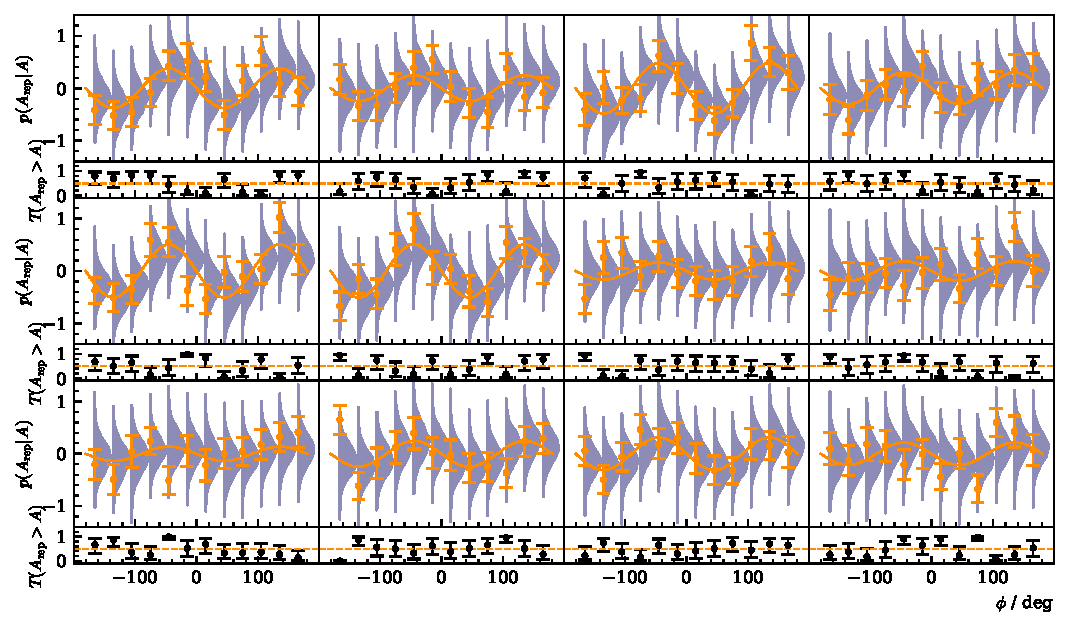
\includegraphics[width=\linewidth]{../bayes/toyMC/plots/toyMC_ppd_checks.pdf}
		\caption{Posterior predictive checks $p\left(A_\text{rep}\big|A\right)$ from a \textsc{Bayesian} fit to the event yield asymmetries for six toy Monte Carlo bins are shown as distributions. The data points in the upper plot are the asymmetry $A\left(\phi\right)$, which was additionally fitted using a $\chi^2$ fit (solid line). The goodness of fit is shown using $p$-values, which give the fraction $T\left(A_\text{rep}>A\right)$ of replicated samples greater than the original measured value, with propagated statistical error bars on the bottom of each plot. The expected mean value of $T\left(A_\text{rep}>A\right)=0.5$ is indicated by the dashed line. }
		\label{fig:toymc_asym}
	\end{sidewaysfigure}




\begin{figure}[htbp]
	\centering
	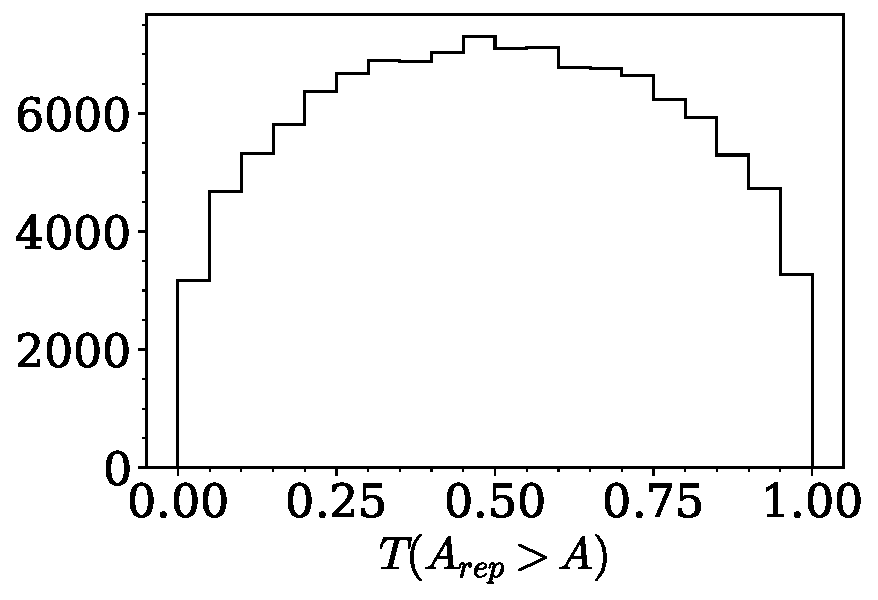
\includegraphics[width=\linewidth]{../bayes/toyMC/plots/toyMC_pval_hist.pdf}
	\caption{$p$ values of all toy Monte Carlo bins. They are centered around their mean at $0.5$, which is indicated by the dashed line, and show no bias towards higher or lower values, thus confirming an adequate fit.}
	\label{fig:toymc_pvals}
\end{figure}

\noindent To check whether the fit is unbiased and provides correct error estimation one can investigate the normalized residuals
\begin{equation}
	\xi = \frac{\Sigma^\text{fit}-\Sigma^\text{true}}{\Delta\Sigma^\text{fit}}
	\label{eq:res}
\end{equation}
 in the case of a least-squares fit. Here $\Sigma^\text{fit}$ and $\Delta\Sigma^\text{fit}$ are the value and corresponding statistical error for the beam asymmetry as obtained from the fit and $\Sigma^\text{true}$ is the true value that was used to throw the toy MC experiments. An unbiased fit with right estimation of errors yields \cite{statistics} \begin{equation}
	\xi\sim\mathcal{N}\left(0,1\right).
	\label{eq:xi}
\end{equation}
This criterion obviously cannot be applied in the same way to a \textsc{Bayesian} fit. The fit results are distributions and therefore lack point estimates $\Sigma^\text{fit}$ and errors $\Delta\Sigma^\text{fit}$. However, one can modify Equation \eqref{eq:res} to the needs of a \textsc{Bayesian} fit to assess its performance:
\begin{equation}
	\Xi=\frac{\text{median}\left(\left\{\Sigma^\text{fit}\right\}\right)-\Sigma^\text{true}}{\text{std}\left(\left\{\Sigma^\text{fit}\right\}\right)}\sim\mathcal{N}(0,1).
\end{equation}
Instead of the point estimates $\Sigma^\text{fit}$ the median of the set of all draws from the marginal posteriors $\left\{\Sigma^\text{fit}\right\}$ is shifted by the true value $\Sigma_\text{true}$ and normalized by the standard deviation as an error estimate for each fit. Although this is not a rigorously derived quantity it allows to identify possible bias if $\text{mean}\left(\Xi\right)\neq 0$. Furthermore, checking that $\sigma\approx1$ will affirm whether the width of the marginal posterior distributions is sensible. Figure \ref{fig:toymcpost} shows the combined $\Xi$-distributions of all fits and the unaltered combined posteriors shifted by the true value. As expected, both distributions are normal as a \textsc{Gaussian} fit proves.  
\begin{figure}[htbp]
	\centering
	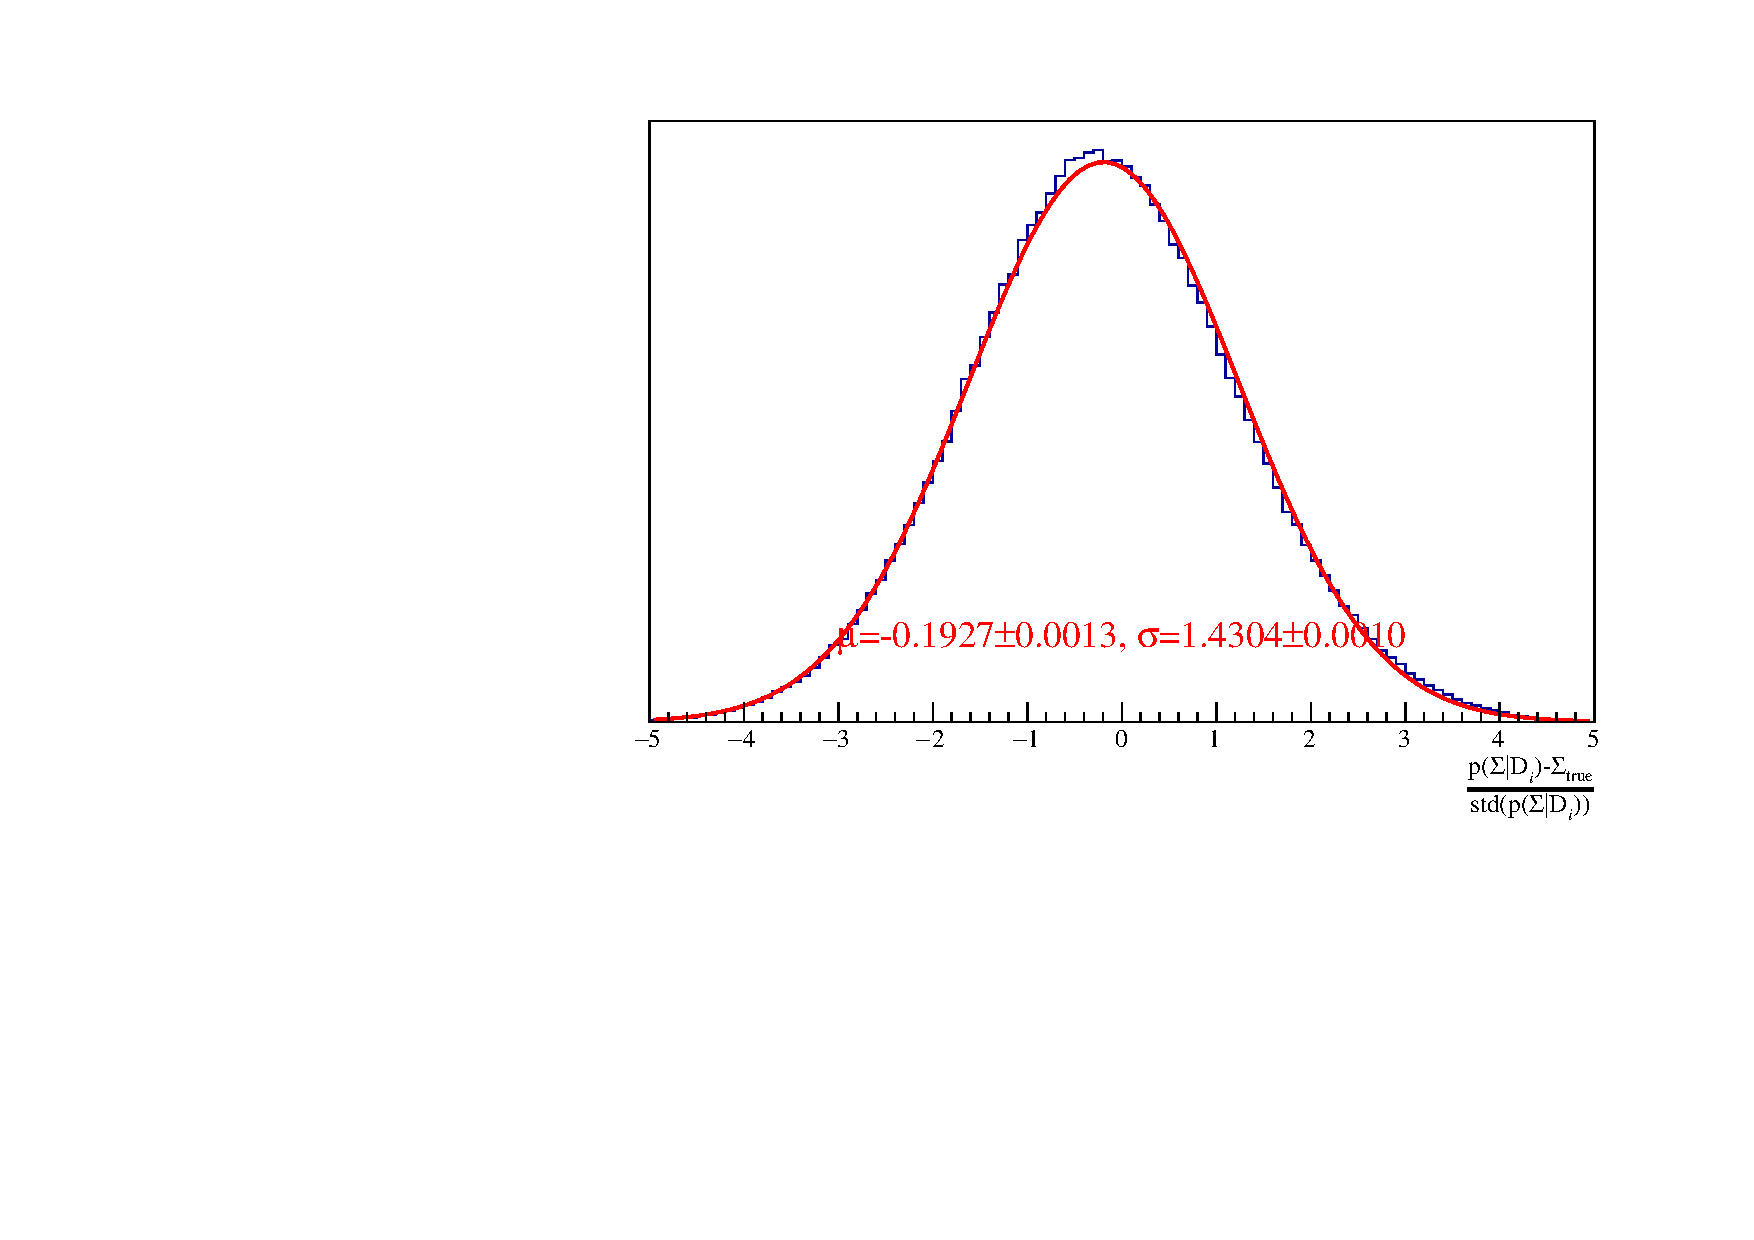
\includegraphics[width=.49\linewidth]{../bayes/toyMC/plots/combined_post_add.pdf}
	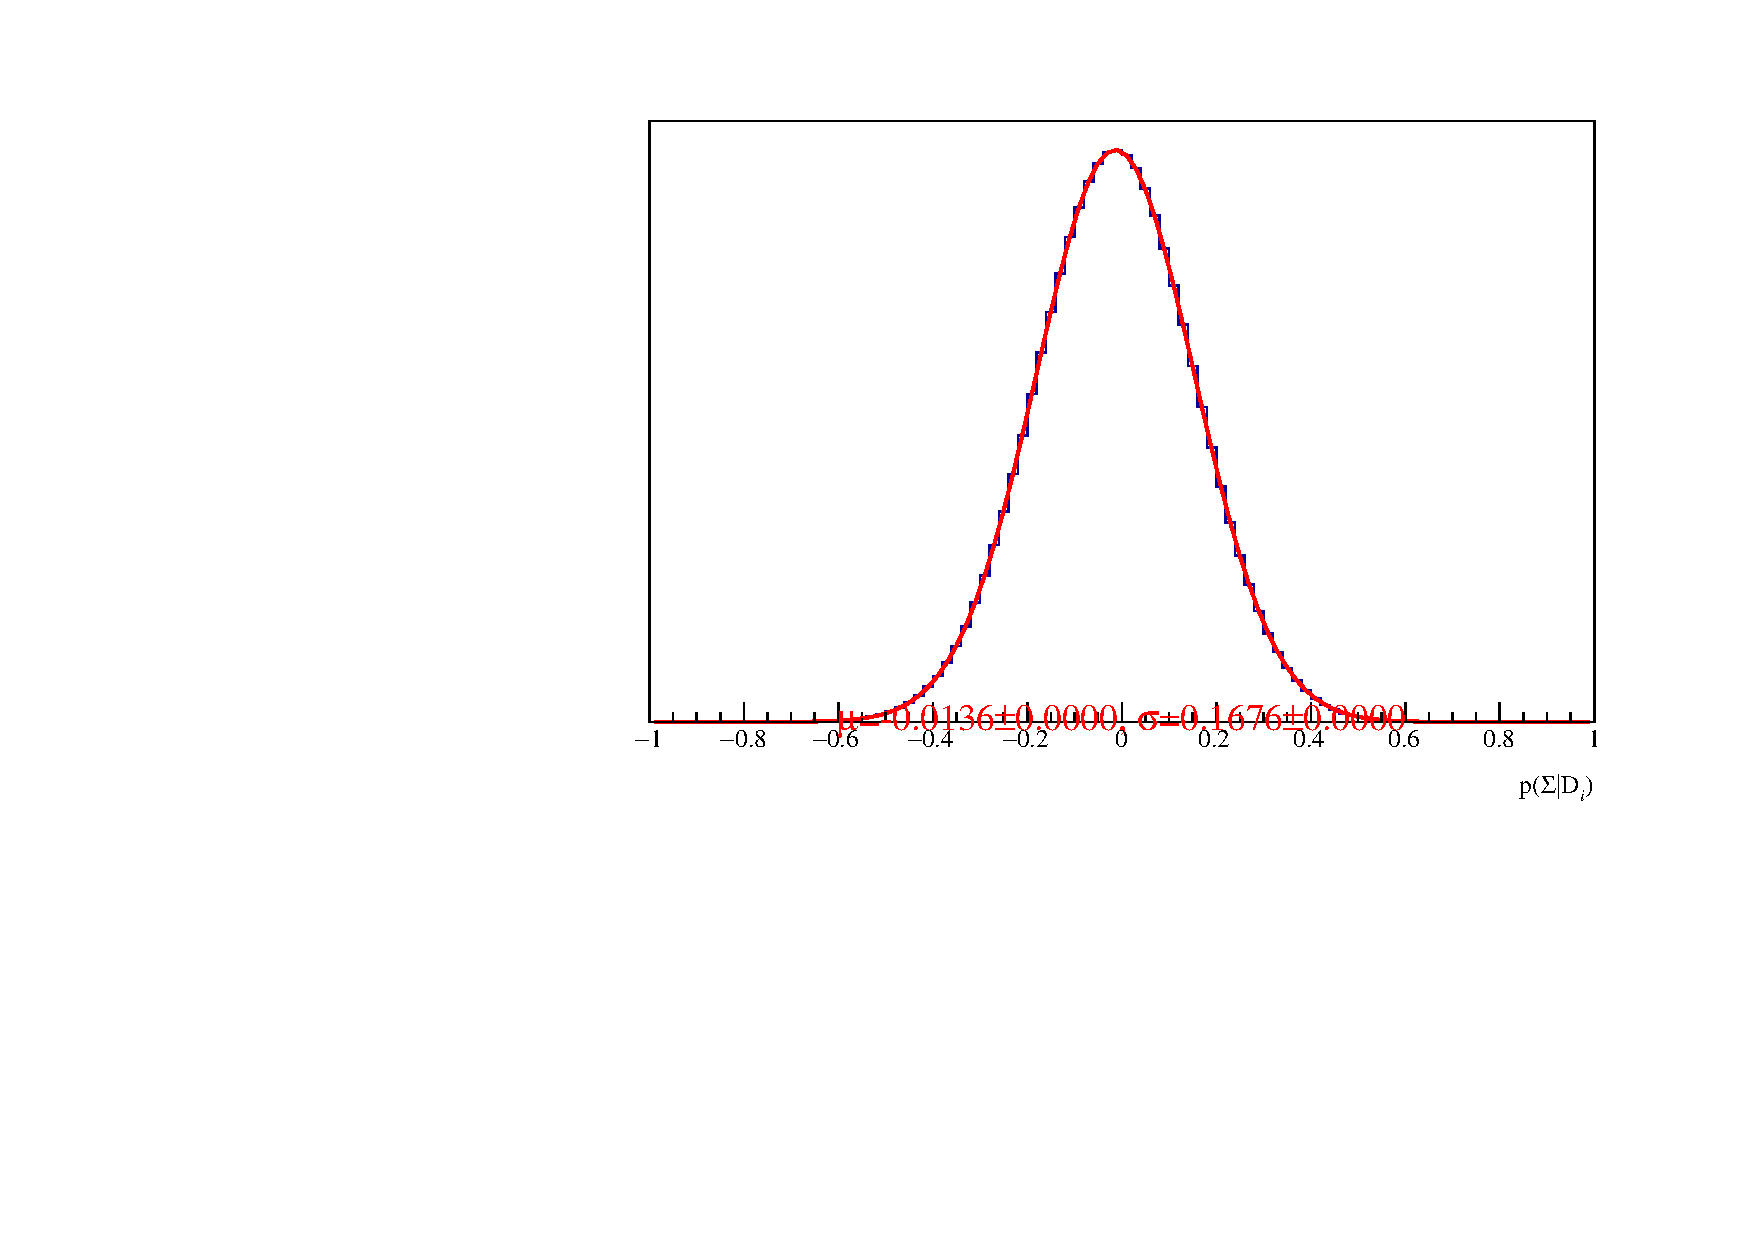
\includegraphics[width=.49\linewidth]{../bayes/toyMC/plots/combined_post_add_raw.pdf}
	\caption{Left: Combined posterior distributions of all $10000$ fits normalized by their respective standard deviation. Right: Unaltered combined posterior distributions of all $10000$ fits. A \textsc{Gaussian} fit was performed to determine mean $\mu$ and standard deviation $\sigma$ of the distributions with results given on top.}
	\label{fig:toymcpost}
\end{figure}
The width of the marginal posterior distributions can be regarded as sensible since the standard deviation of the $\Xi$ distribution $\sigma_\Xi\approx1$\footnote{One cannot expect to fulfill Eq. \eqref{eq:xi} exactly, since the errors are after all only estimates that aim to create comparability to the least squares fit.}. This is furthermore confirmed by the fact that $\left\{\Sigma^\text{fit}\right\}-\Sigma^\text{true}=0$ within one standard deviation. Yet, the fit results tend to underestimate the beam asymmetry, because both distributions are centered out of their statistical error at $\mu\pm\Delta\mu<0$. This indicates bias towards smaller values of the beam asymmetry. Remarkably, this bias is \emph{not} introduced by the \textsc{Bayesian} fit, but by the choice of binning and available statistics as an extensive investigation of binned fits (least squares and \textsc{Bayesian}) to toy Monte Carlo data showed. A detailed discussion thereof is given in appendix \ref{app:binnedfits}. For now it suffices to note the origin of this bias lies in the choice of binning and is thus inevitable. And, most importantly, the introduced bias is negligible compared to the width of the posterior distributions, so that a binned fit will produce valid fit results in any case. Nevertheless this emphasizes the advantage of unbinned fitting, which is discussed in the next paragraph.

It has been established that the fit produces valid results with sensible statistical errors, i.e. widths of posterior distributions, and the description of the data is in agreement with the expectations. It remains to diagnose the convergence of the \textsc{Markov} chains to finally deem the binned fit method appropriate. For this the $\widehat{R}$ value and the relative Monte Carlo standard error (MCSE) $\frac{\sigma_\text{MCSE}}{\text{median}\left[p\left(\Sigma|y\right)\right]}$ that were introduced in section \ref{sec:bayes} are investigated. If $\widehat{R}<1.05$ one can assume that the different chains have converged and explored the same parameter space \cite{rhat}. Furthermore the accuracy supplied by the number of draws from the posteriors can be evaluated with the relative MCSE. It is demanded that $\frac{\sigma_\text{MCSE}}{\text{median}\left[p\left(\Sigma|y\right)\right]}\lesssim 5\%$. This is the case for $97\%$ of all fits, see Figure \ref{fig:toyMC_diagnostics} on the left. When the fit result for the beam asymmetry is close to $0$ larger values for the relative MCSE are observed. The $\widehat{R}$ values (Figure \ref{fig:toyMC_diagnostics} on the right) clearly indicate good within and between chain convergence. This means that the hyper parameters $n_\text{chain},n_\text{samples}$ and $n_\text{warm up}$ as chosen are well tuned, although one may increase the number of sample draws from the posterior for the fit from measured data to further suppress the relative MCSE. Then, only $11\cdot12$  as opposed to $10000$ fits have to be performed keeping the computational cost reasonable.    
\begin{figure}[htbp]
	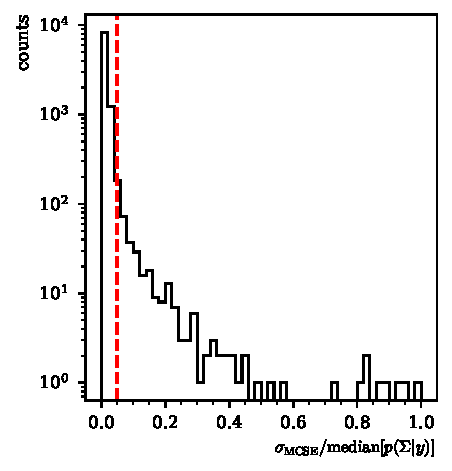
\includegraphics[width=.49\linewidth]{../bayes/toyMC/plots/toyMC_mcse_hist.pdf}
	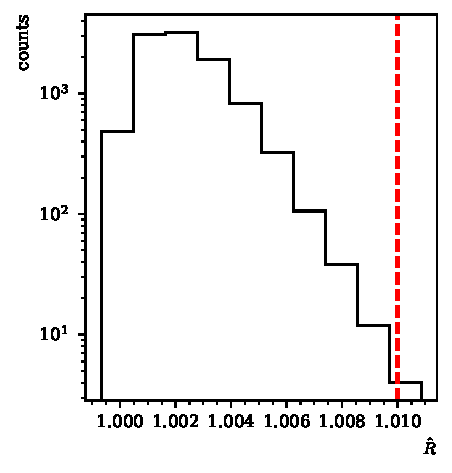
\includegraphics[width=.49\linewidth]{../bayes/toyMC/plots/toyMC_rhat_hist.pdf}
	\caption{ Left: relative error $\frac{\sigma_\text{MCSE}}{\text{median}\left[p\left(\Sigma|y\right)\right]}$ Right: $\widehat{R}$ associated with the fit parameter $\Sigma$. Both are shown for all 10000 fits. The critical values that should not be exceeded are marked by dashed lines.}
	\label{fig:toyMC_diagnostics}
\end{figure}
\subsubsection{Event based fit}
Not only signal events but also contributions from random time background as well as the imperfect detector efficiency $\epsilon(\phi)$ have to be simulated in order to test the method of event based fitting. For each polarization setting prompt peak and sideband events are drawn from the theoretical $\phi$-distributions $p_\text{prompt}$ and $p_\text{sideband}$ which are given in Equations \eqref{eq:pprmpt} and \eqref{eq:pside}. The total number of draws per setting and bin is again given by \textsc{Poisson} distributions and the ratio of prompt peak to sideband events is given by the time cut weights $\left\{w_i\right\}_{i=1}^7$ employed for the actual analysis of the $p\eta$ final state data \cite{farahphd}. This means that seven times prompt peak and sideband events need to simulated. The fraction of background events within the prompt peak $f$ was set to $f=0.95$. Further, the values $p_\gamma^\parallel=0.25,p_\gamma^\bot=0.3,\Sigma=0.5$, $\Sigma^\text{bkg}=-0.5$ and lastly, a random efficiency function as already chosen in reference \cite{farahphd} were appointed. Finally the hyperparameters $n_\text{chain},n_\text{samples},n_\text{warm up}$ are chosen the same as previously. Table \ref{tab:mcsum} shows a summary of all toy Monte Carlo properties.
\begin{table}[htbp]

	\renewcommand{\arraystretch}{1.5}
	\centering
	\begin{tabularx}{\linewidth}{l|XXX}
		\toprule
		\textbf{chosen parameters} & \multicolumn{3}{l}{$p_\gamma^\parallel=0.25,p_\gamma^\bot=0.3,\Sigma=0.5$, $\Sigma^\text{bkg}=-0.5$, $f=0.95$,}\\ &\multicolumn{3}{l}{$w_1=\frac{15}{210},w_2=\frac{8}{210},w_3=\frac{4}{210},w_4=\frac{10}{210},w_5=\frac{14}{210},w_6=\frac{6}{210},w_7=\frac{11}{210}$}\\
		\hline
		\textbf{simulation draws} &\multicolumn{3}{c}{$7\cdot N^\parallel_{\text{total},i}\sim\mathcal{P}(800)$, $7\cdot N^\bot_{\text{total},i}\sim\mathcal{P}(1000)\quad\big|_{i=1}^7$}\\
		\cline{2-4}
		&signal in prompt&background in prompt& sideband \\
		&$N^{\parallel/\bot}_\text{total}\cdot f$&$N^{\parallel/\bot}_\text{total}\cdot\left(1-f\right)$&$N^{\parallel/\bot}_\text{total}\cdot\left(1-f\right)\cdot1/w_i$\\
		\hline
		\textbf{efficiency function}&\multicolumn{3}{l}{$\epsilon\left(\phi\right)=1/10.5\cdot\left(9.3+0.28\cdot\cos\phi+0.24\cdot\sin3\phi\right)$}\\
		\hline
		\textbf{hyperparameters}&\multicolumn{3}{l}{$n_\text{samples}=1000,n_\text{chain}=4,n_\text{warm up}=1000$}\\
		\bottomrule
	\end{tabularx}
	\caption{Summary of the complete setting of all toy Monte Carlo experiments for the event based fit. Values and table layout adapted from \cite{farahphd}.}
	\label{tab:mcsum}
\end{table}
In total, 1000 toy Monte Carlo experiments are thrown. To evaluate the fit results only the posterior distributions are available. As before, the residuals $\Xi$ are built from all fits, now for $\Sigma$ as well as $\Sigma^\text{bkg}$. They are shown in Figure \ref{fig:toyMCposteriors} together with the unnormalized posterior distributions. 
\begin{figure}[htbp]
	\centering
	\begin{subfigure}{\linewidth}
		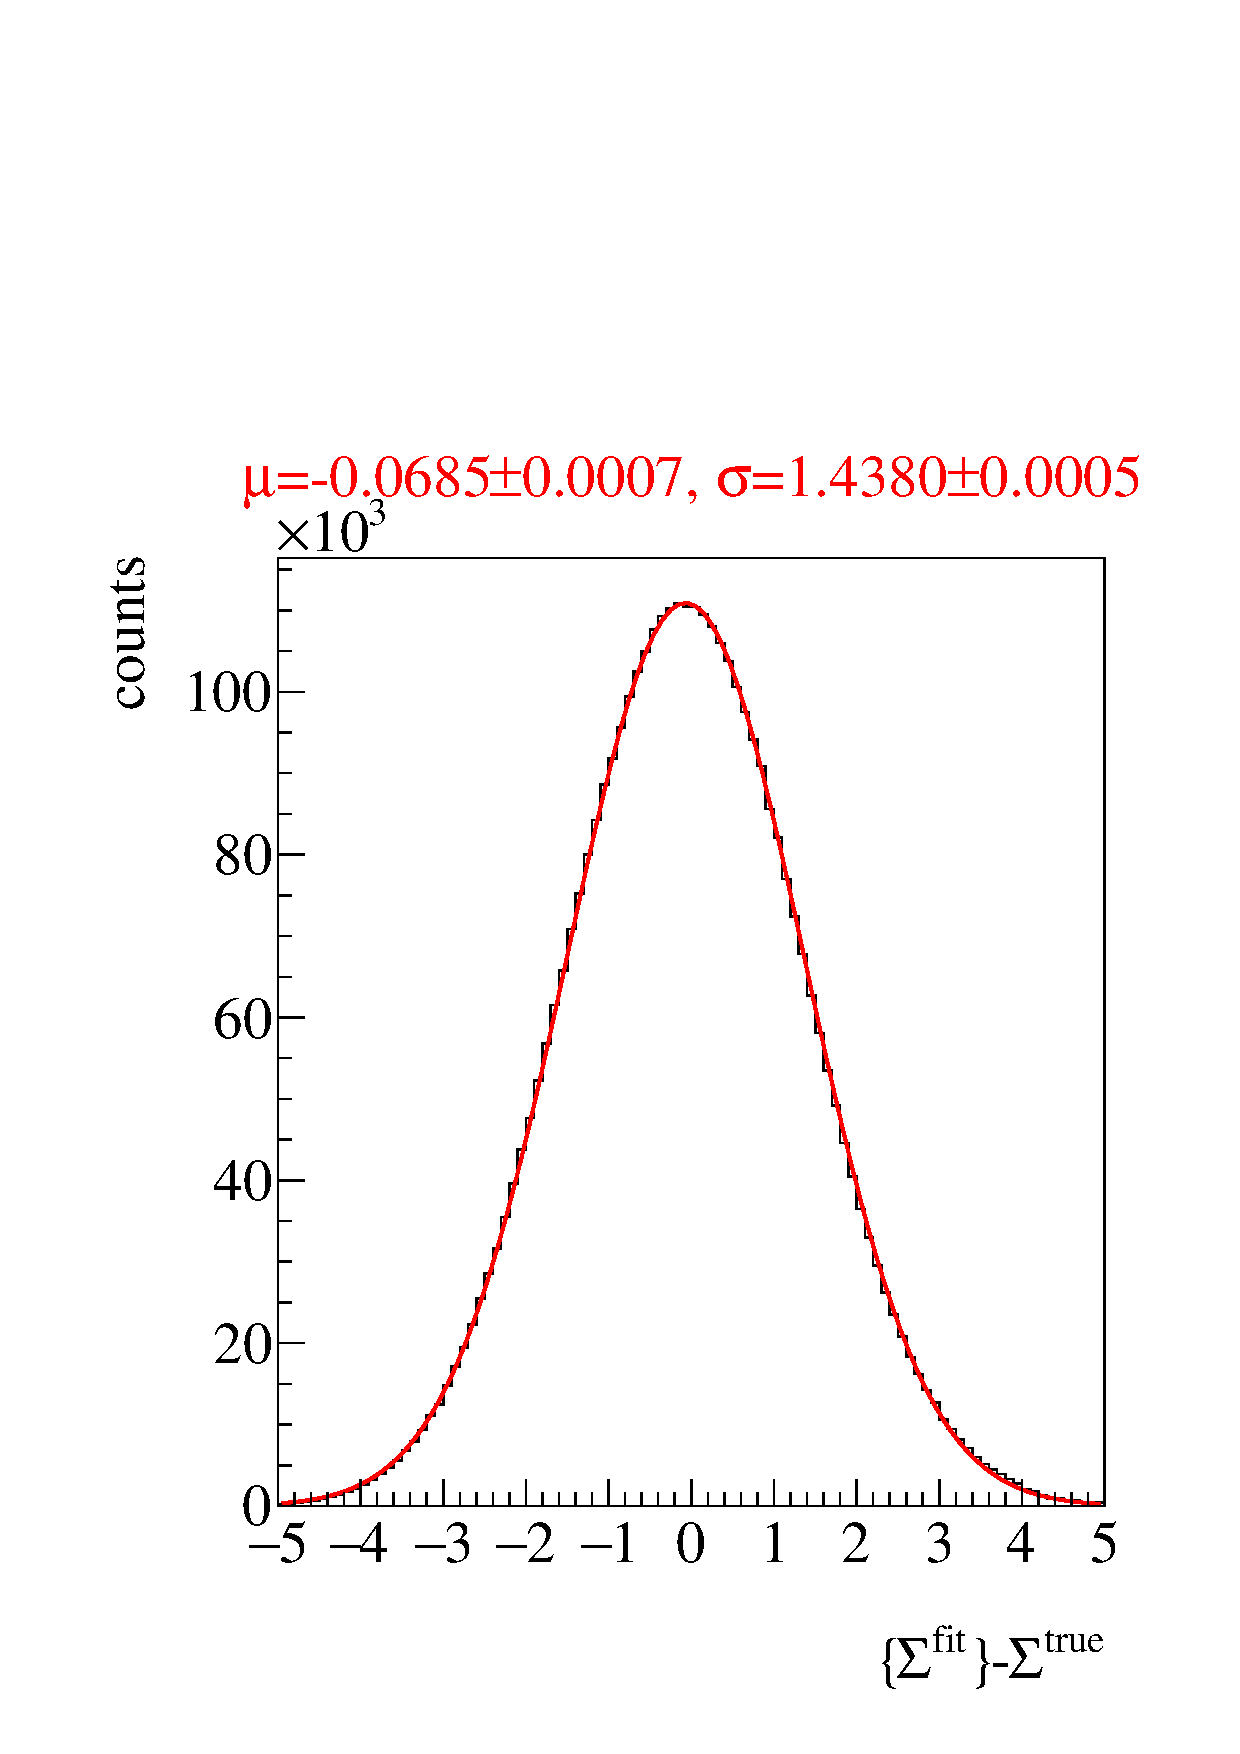
\includegraphics[width=.49\linewidth]{../bayes/event_based_fit/plots/combined_post_add.pdf}
		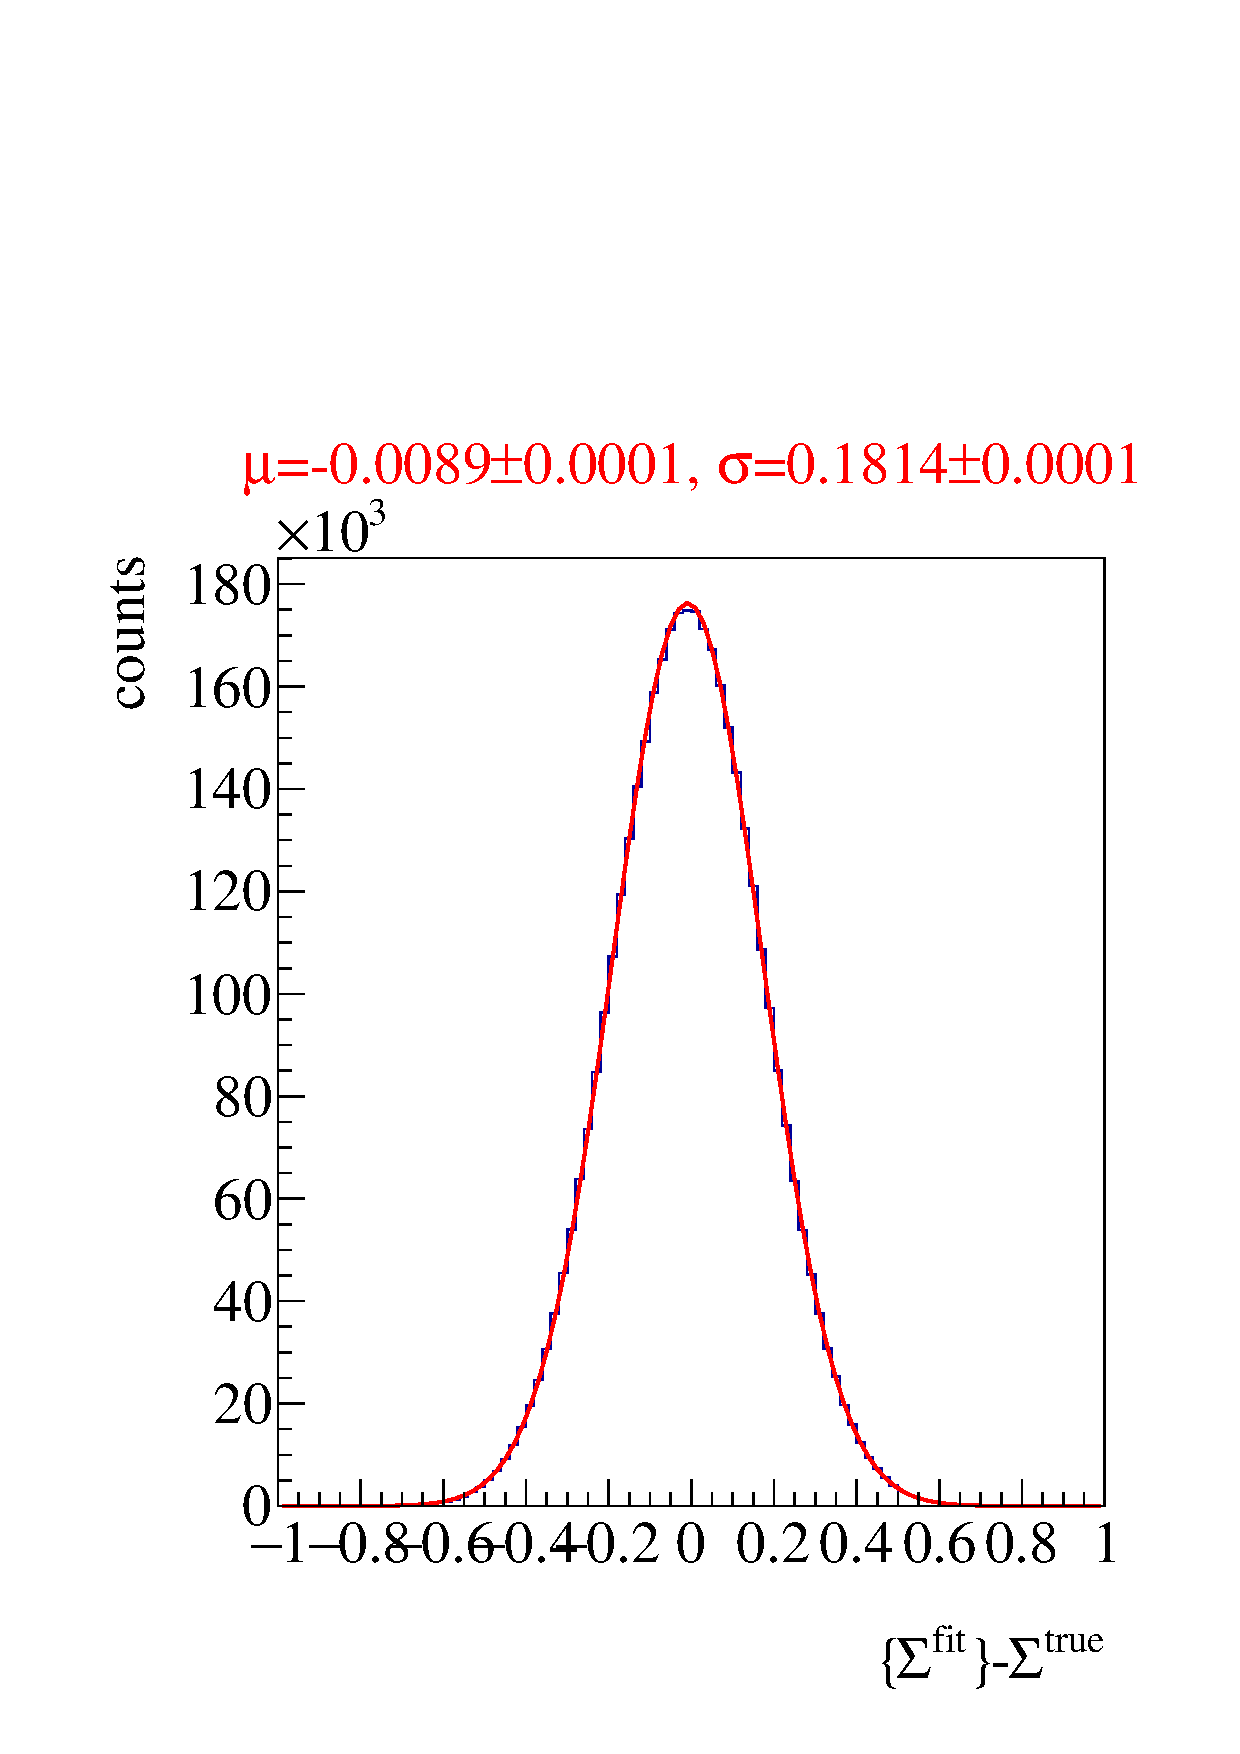
\includegraphics[width=.49\linewidth]{../bayes/event_based_fit/plots/combined_post_add_raw.pdf}
		\subcaption{Signal beam asymmetry $\Sigma$}
	\end{subfigure}
	\begin{subfigure}{\linewidth}
		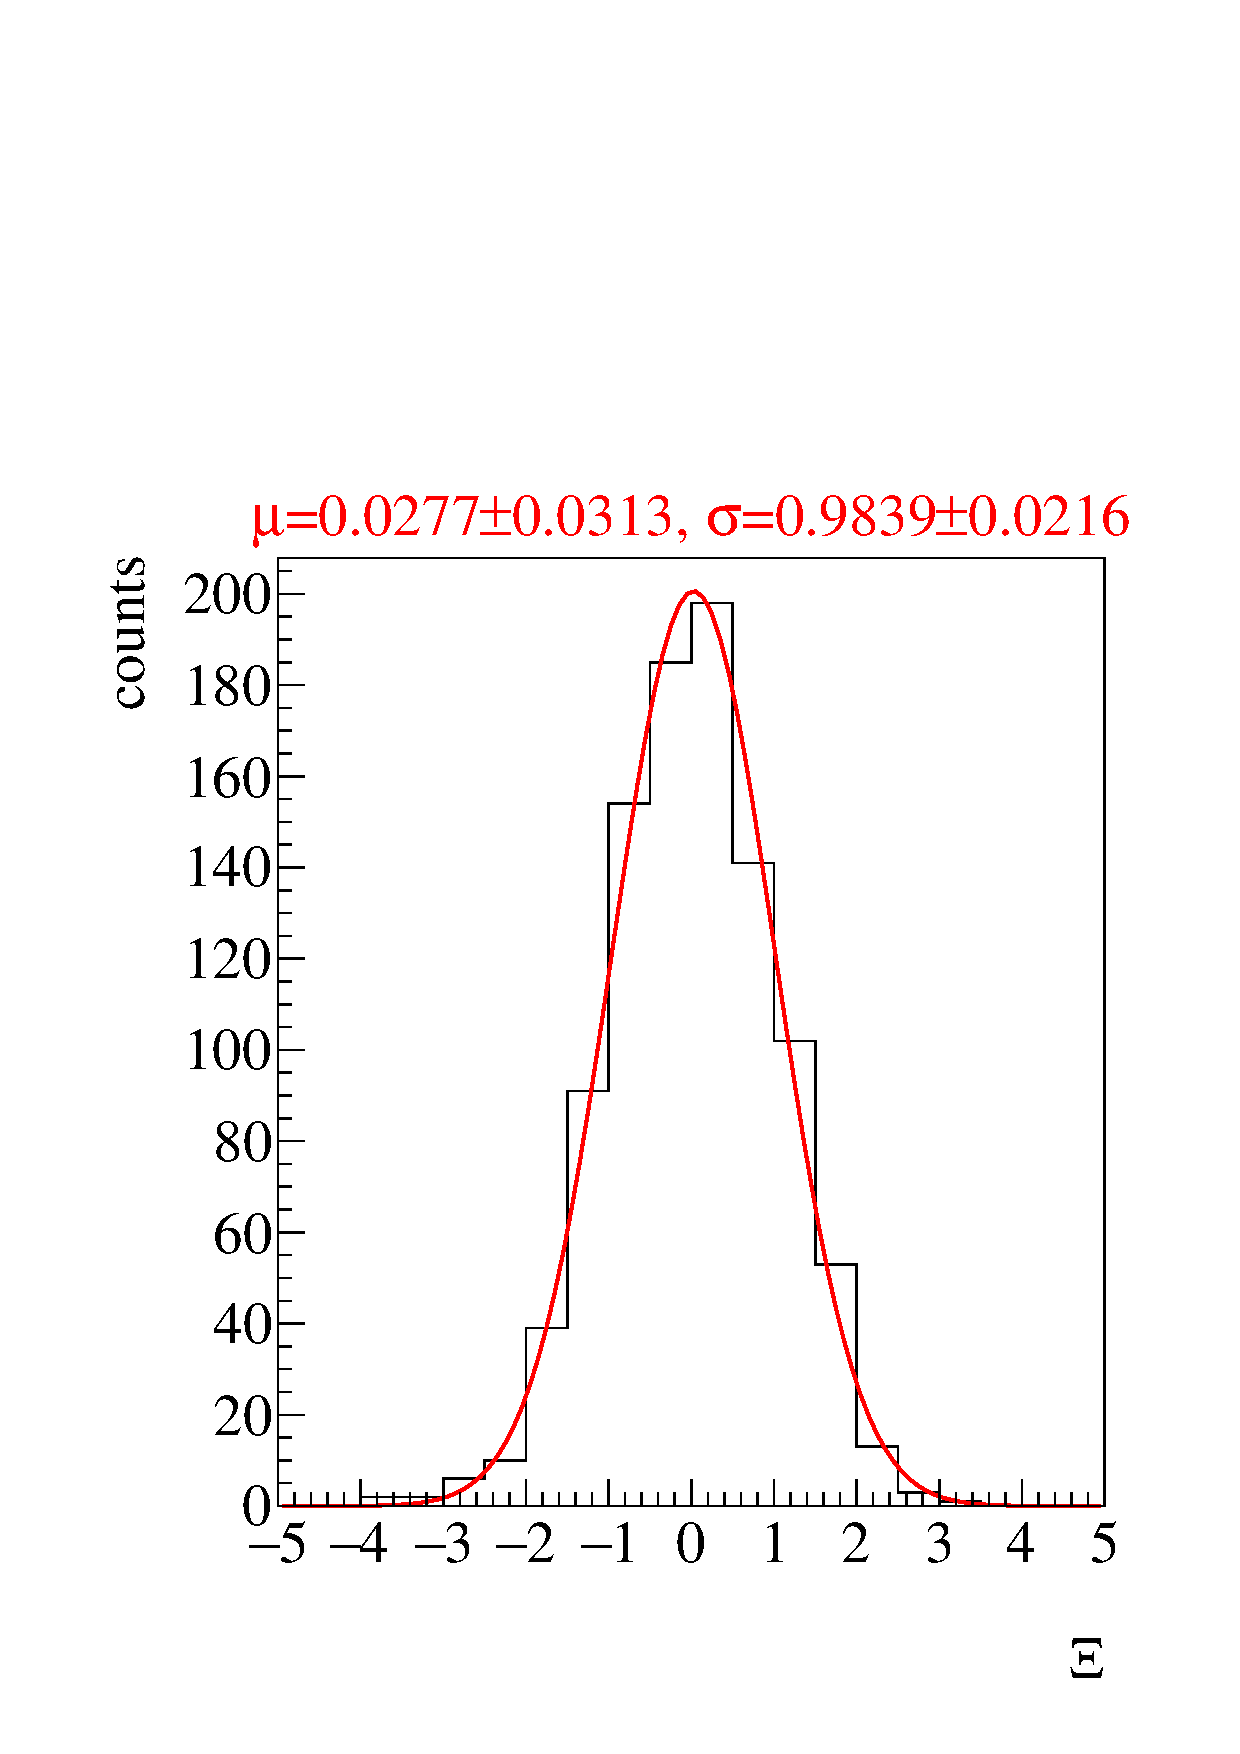
\includegraphics[width=.49\linewidth]{../bayes/event_based_fit/plots/combined_post_add_bkg.pdf}
		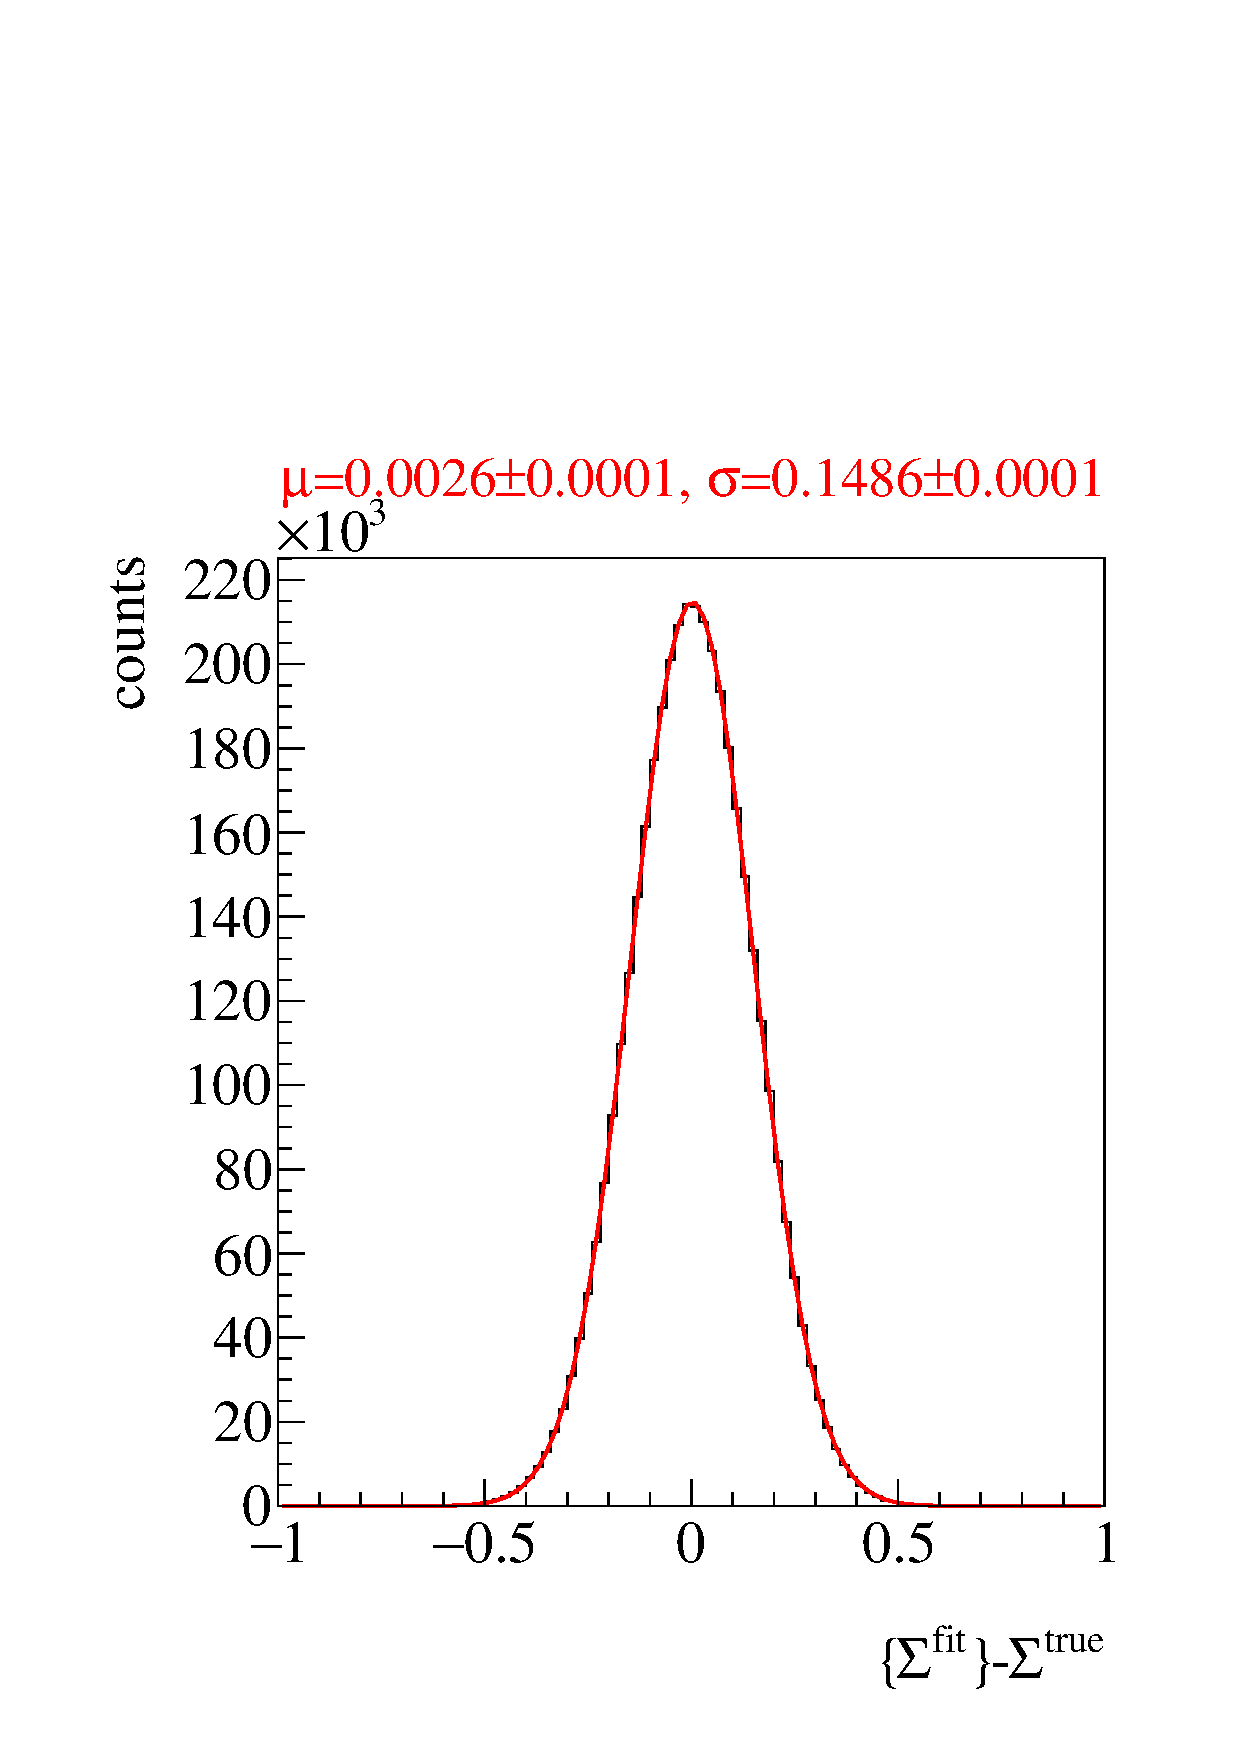
\includegraphics[width=.49\linewidth]{../bayes/event_based_fit/plots/combined_post_add_raw_bkg.pdf}
		\subcaption{Background beam asymmetry $\Sigma^\text{bkg}$}
	\end{subfigure}
	\caption{Combined posteriors for the beam asymmetries $\Sigma$ and $\Sigma^\text{bkg}$ from all 1000 event based fits. Left: Residuals $\Xi$ Right: Unnormalized posterior distributions. A \textsc{Gaussian} fit is performed on the distributions with results for mean $\mu$ and standard deviation $\sigma$ on top.}
	\label{fig:toyMCposteriors}
\end{figure}
Note that the distributions are truncated towards the tails at $\Sigma\to1$ and $\Sigma^\text{bkg}\to-1$ as implemented in the \textsc{Bayesian} fit in Stan. Also the event based fit is able to reproduce the true values within one standard deviation of the posterior distribution $\sigma_\text{posterior}$. Only slight bias towards smaller values of the signal beam asymmetry is seen, but again with negligible effect on the results in comparison to the widths of the distributions. Additionally, the mean of the distributions are 0 within $3\sigma$ of their statistical error and the errors are estimated correctly, since $\sigma_\text{posterior}=1$ within the statistical error. Note that the background beam asymmetry is estimated closer to its true value than the signal beam asymmetry because there are more random background events than signal events.

If the total amount of posterior distributions is not too large one might also combine them in a \emph{pooled likelihood} approach (see subsection \ref{subsec:combinf}). This is shown in Figure \ref{fig:poollik} for both determined asymmetries.
\begin{figure}[htbp]
	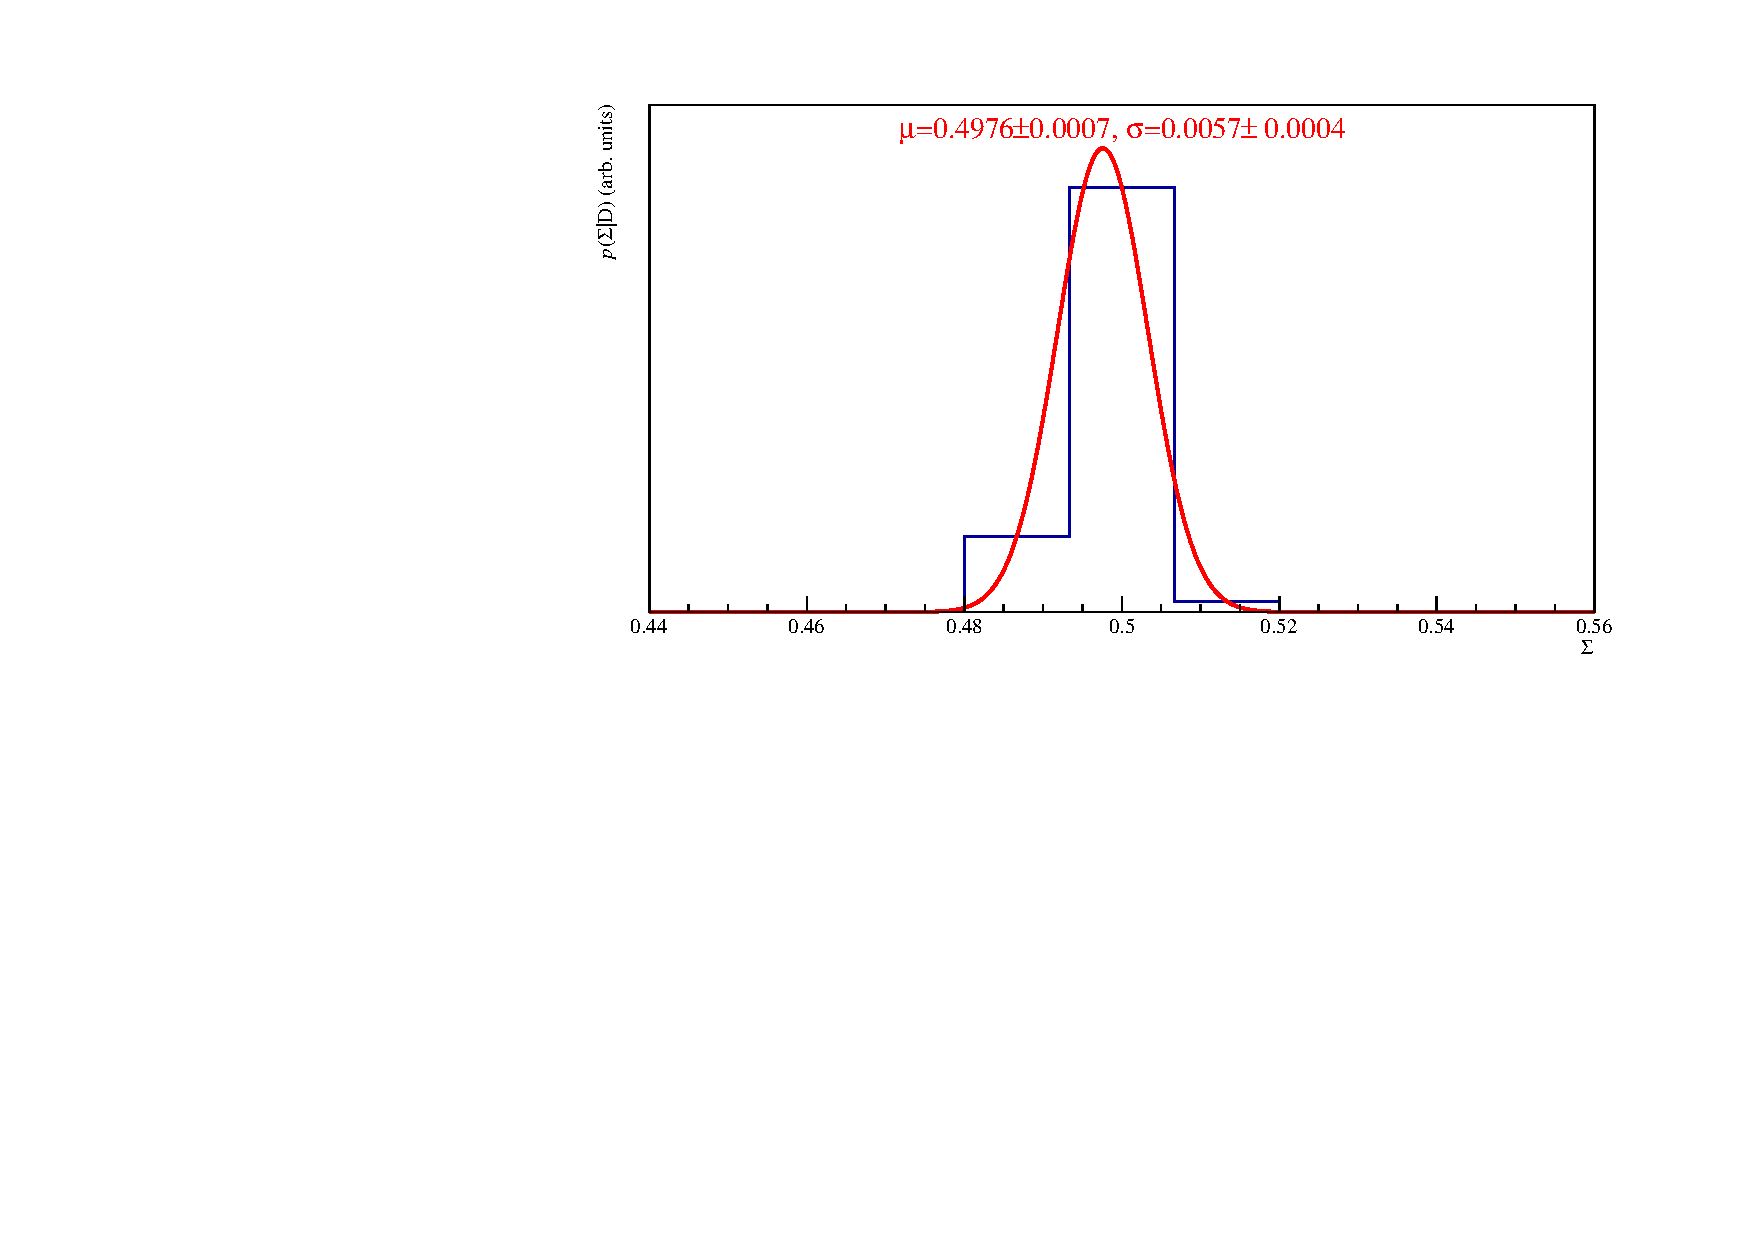
\includegraphics[width=.49\linewidth]{../bayes/event_based_fit/plots/combined_post_mul.pdf}
	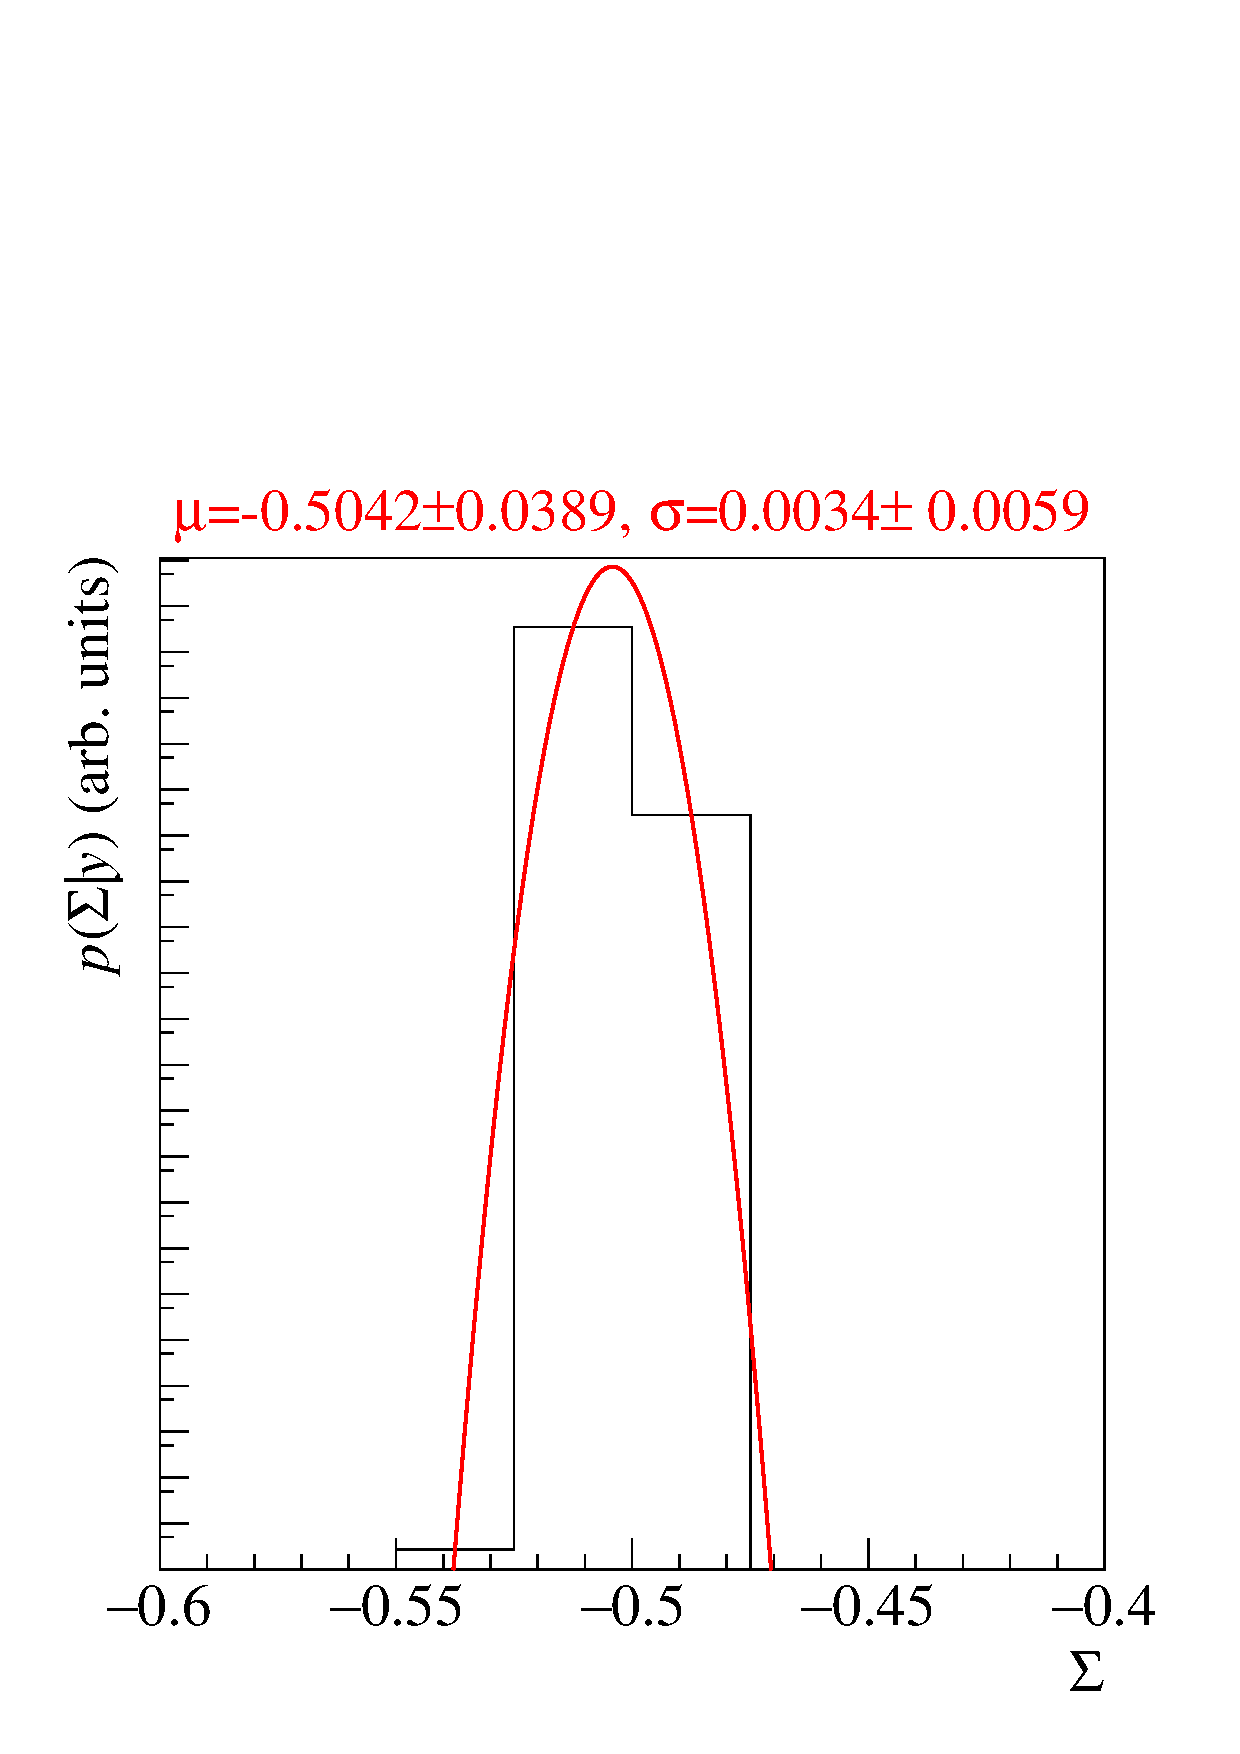
\includegraphics[width=.49\linewidth]{../bayes/event_based_fit/plots/combined_post_mul_bkg.pdf}
	\caption{Combined posterior probabilities using the \emph{pooled likelihood} approach. Left: Signal beam asymmetry, Right: background beam asymmetry. Mean and standard deviation as obtained from a \text{Gaussian} fit are shown on top}
	\label{fig:poollik}
\end{figure}
 Because the true asymmetries are within $1\sigma$ of the resulting distribution one can finally conclude that the event based fit estimates positions and widths of the posterior distributions correctly. 
 
 A check of the relative MCSE and $\widehat{R}$ values as shown in Figure \ref{fig:toyMC_diagnostics1} reveals also that the hyperparameters $n_\text{chain},n_\text{samples},n_\text{warm up}$ are correctly tuned.
 \begin{figure}[htbp]
 	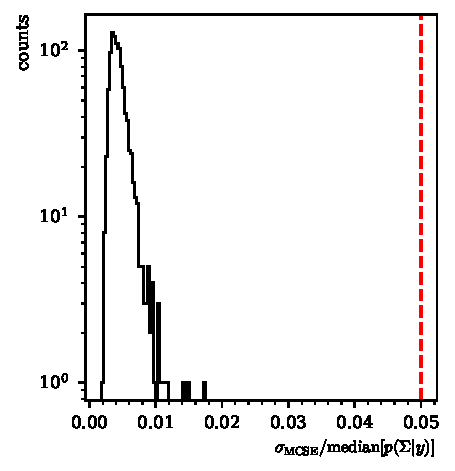
\includegraphics[width=.49\linewidth]{../bayes/event_based_fit/plots/toyMC_mcse_hist.pdf}
 	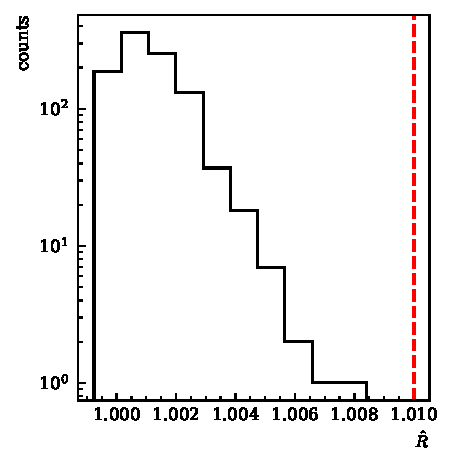
\includegraphics[width=.49\linewidth]{../bayes/event_based_fit/plots/toyMC_rhat_hist.pdf}
 	\caption{ Left: relative error $\frac{\sigma_\text{MCSE}}{\text{median}\left[p\left(\Sigma|y\right)\right]}$ Right: $\widehat{R}$ associated with the fit parameter $\Sigma$. Both are shown for all 1000 fits. The critical values that should not be exceeded are marked by dashed lines.}
 	\label{fig:toyMC_diagnostics1}
 \end{figure}
It is noteworthy that the event based fit creates more precise results although less Monte Carlo experiments in total were performed than for the binned fit. 

Next to signal and background beam asymmetry the fit also estimates an efficiency function $\epsilon(\phi)$ that is described by a \textsc{Fourier} series. The polarization weighted sum of event yields allows to confirm whether a good description of the efficiency is achieved because it is given by the efficiency function modulated only by a constant, see previous section \ref{sec:meth} $\alpha \tilde{N}^\parallel + \beta\tilde{N}^\bot = c\cdot\epsilon\left(\phi\right).$ Figure \ref{fig:toyMC_eff_func} shows the weighted sum of event yields with the same binning as used in the binned fit together with a posterior predictive check using the draws of all parameters distributions $a,b$. 
\begin{figure}[htbp]
	\centering
	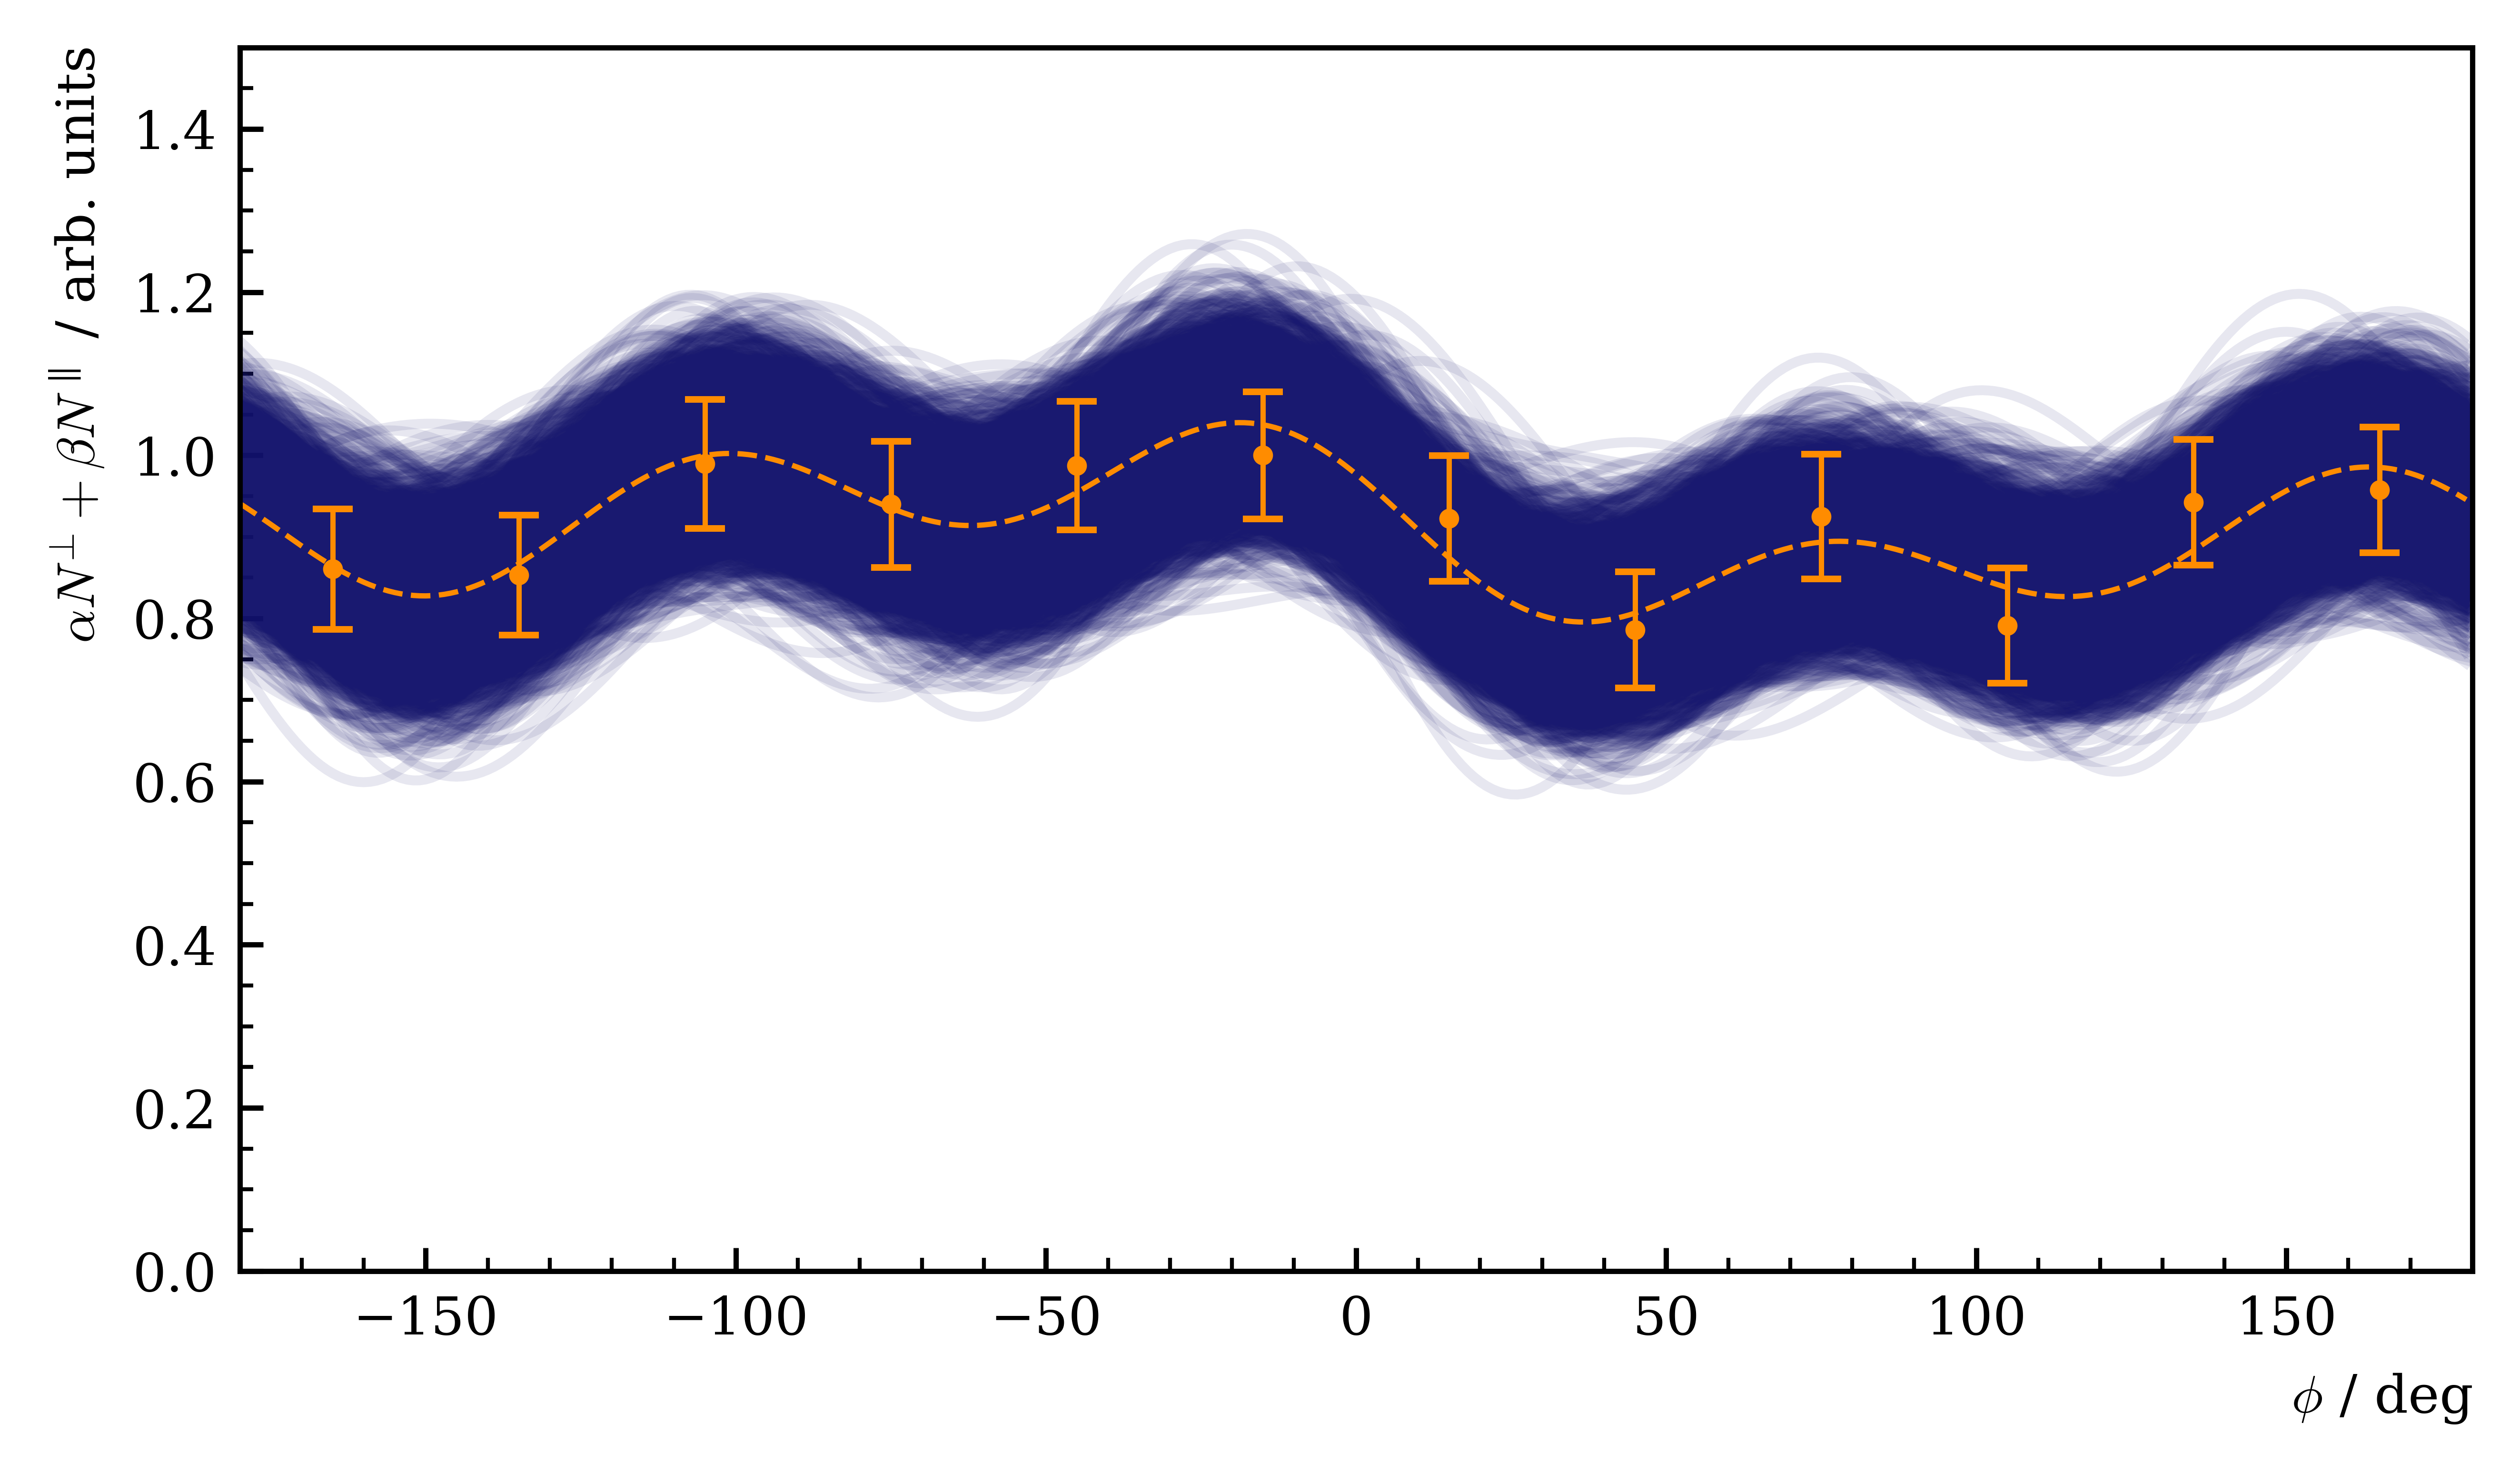
\includegraphics[width=\linewidth]{../bayes/event_based_fit/plots/toyMC_eff_PPC.png}
	\caption{Posterior predictive check using the draws of the detector coefficients $a$ and $b$. Points with error bars are the polarization weighted sum of event yields. The dashed line is the mean of the predictive values while the solid opaque lines are representative of one simulation draw $a^{(s)},b^{(s)}$.}
	\label{fig:toyMC_eff_func}
\end{figure}
As opposed to the binned fit it is not only performed at each data point but for significantly more points. This mimics a continuous function as is appropriate for an unbinned fit. However, for better visibility the posterior predictive distributions are not built at every point but the efficiency function is plotted for each set of draws $a^{(s)},b^{(s)}, s=1\dots4000$. No $p$ values are estimated since they would not be representative of the whole fit. The mean of the posterior predictive distributions is given by the dashed line and agrees within statistical error bars with the simulated data.
\newpage
\subsection{Application of methods to data}
Since both methods were tested successfully using toy Monte Carlo data, both are subsequently applied to real data to extract the beam asymmetry. Since the number of fits is small compared to the amount of fits performed during testing, the amount of posterior draws was increased to $5000$ per chain. All other hyperparameters were left the same
\begin{align}
	n_\text{samples}=5000 && n_\text{chain}=4 && n_\text{warm up}=1000.
\end{align}
\subsubsection{Event yield asymmetries}
In all bins of beam energy and meson polar angle the binned fit was performed. Similar to the Monte Carlo samples, 12 bins in phi are built to comply with the binning in reference \cite{farahphd}, and guarantee comparability.

Figure \ref{fig:asym} shows the resulting asymmetry $A(\phi)$ for all angular bins for the energy bin $\SI{1250}{\mega\eV}\leq E_\gamma<\SI{1310}{\mega\eV}$ as orange data points with statistical error bars.  Additionally shown is a $\chi^2$ fit (orange line) to the asymmetry together with posterior predictive checks as obtained from a fully \textsc{Bayesian} fit according to the introduced model (blue distributions). The goodness of fit is checked via the introduced $p$-values $p=T(A_\text{rep}>A)$, and are shown as black points with propagated error bars on the bottom. The optimal value of $p=0.5$ is marked by the dashed line and realizes the mean of the distribution of all $p$-values, so that one can assume good description of the data by the fits, see Figure \ref{fig:pvals}. This replaces the investigation of the $\chi^2/\text{NDF}$ distribution in the case of a frequentist fit.   
\newpage

	\begin{sidewaysfigure}[htbp]
		\centering
		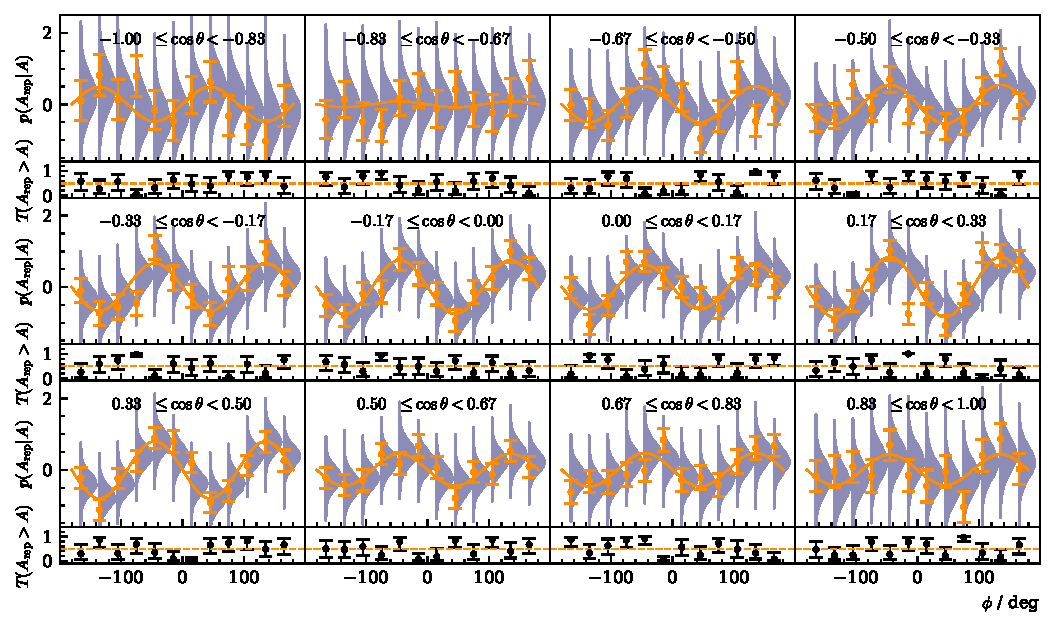
\includegraphics[width=\linewidth]{../bayes/realdeal/plots/ppd_checks.pdf}
		\caption{Posterior predictive checks $p\left(A_\text{rep}\big|A\right)$ from a \textsc{Bayesian} fit to the event yield asymmetries for all angular bins of the energy bin $\SI{1250}{\mega\eV}\leq E_\gamma<\SI{1310}{\mega\eV}$. The data points in the upper plot are the asymmetry $A\left(\phi\right)$, which was additionally fitted using a $\chi^2$ fit (solid line). The goodness of fit is shown using $p$-values, which give the fraction $T\left(A_\text{rep}>A\right)$ of replicated samples greater than the original measured value, with propagated statistical error bars on the bottom of each plot. The expected mean value of $T\left(A_\text{rep}>A\right)=0.5$ is indicated by the dashed line. }
		\label{fig:asym}
	\end{sidewaysfigure}

\newpage


\begin{figure}[htbp]
	\centering
	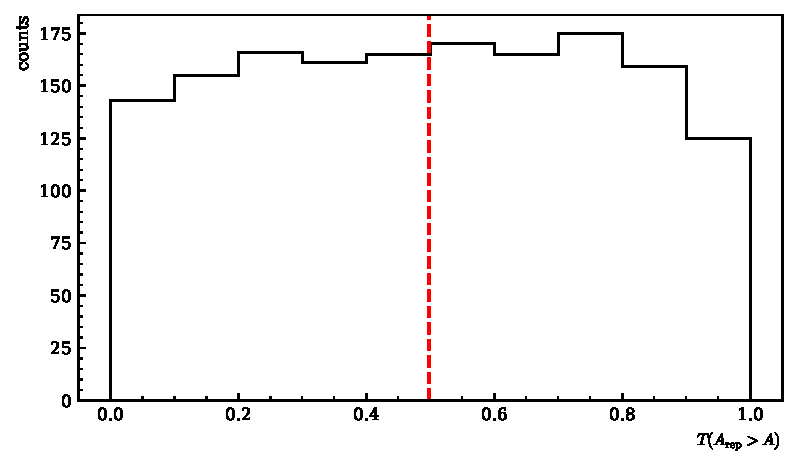
\includegraphics[width=\linewidth]{../bayes/realdeal/plots/pval_hist.pdf}
	\caption{$p$ values generated using all fits. They are centered around their mean at $0.5$, which is indicated by the dashed line, and show no bias towards higher or lower values, thus confirming an adequate fit.}
	\label{fig:pvals}
\end{figure}
The MCMC diagnostics reveal that all \textsc{Markov} chains have converged and explored the available parameter space completely which is characterized by $\widehat{R}=1.00$ for all fits. The increment of posterior draws removed any fluctuations in the $\widehat{R}$ value that was present before. The relative MCSE is below the (self-)defined threshold of $\frac{\sigma_\text{MCSE}}{\text{median}\left[p\left(\Sigma|y\right)\right]}<5\%$ for $95\%$ of all fits. The remaining $5\%$ are fits that estimated the beam asymmetry close to $0$ such that further incrementing the number of posterior draws will not amend this. Both, relative MCSE and $\widehat{R}$ associated with the fit parameter $\Sigma$ of the binned fit, are shown in Figure \ref{fig:diagnostics}. Thus, one can conclude the successful tuning of hyperparemeters concerning the \textsc{Bayesian} fit. 
\begin{figure}[htbp]
	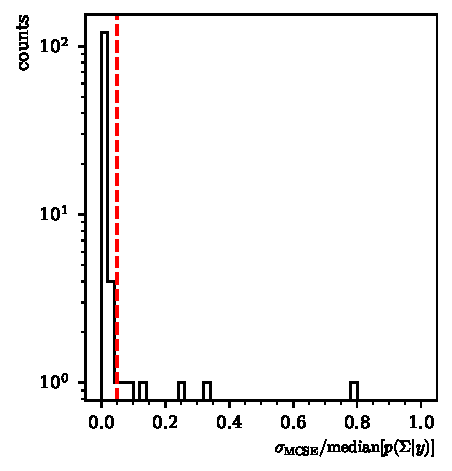
\includegraphics[width=.49\linewidth]{../bayes/realdeal/plots/mcse_hist.pdf}
	\includegraphics[width=.49\linewidth]{../bayes/realdeal/plots/rhat_hist.pdf}
	\caption{ Left: relative error $\frac{\sigma_\text{MCSE}}{\text{median}\left[p\left(\Sigma|y\right)\right]}$ Right: $\widehat{R}$ associated with the fit parameter $\Sigma$. Both are shown for all $11\cdot12$ binned fits to the asymmetry $A\left(\phi\right)$. The critical values that should not be exceeded are marked by dashed lines.}
	\label{fig:diagnostics}
\end{figure}
\subsubsection{Event based fit}
The discussed \textsc{Bayesian} event based fit is also performed for all kinematic bins. The MCMC diagnostics reveal good choice of hyperparameters, as Figure \ref{fig:diagnostics1} shows. As already observed during the toy Monte Carlo experiments, the unbinned fit produces more precise results; $98\%$ of all fits exhibit an MCSE below threshold, those bins with error above threshold are again explained by values of the beam asymmetry $\Sigma\approx0.$ Good within and between chain convergence is reached, as $\widehat{R}=1.00$ for all fits shows.

The only illustrative measure regarding the performance of the unbinned fit is the posterior predictive distribution of the detector coefficients $a,b$. Figure \ref{fig:eff_func} shows the weighted sum of event yields with the same binning as used in the binned fit together with a posterior predictive check using the draws of all parameters distributions $a,b$ for the kinematic bin $\SI{1250}{\mega\eV}\leq E_\gamma<\SI{1310}{\mega\eV}, 0\leq\cos\theta<0.17$. 
As opposed to the binned fit it is not only performed at each data point but for significantly more points. This mimics a continuous function as is appropriate for an unbinned fit. However, for better visibility the posterior predictive distributions are not built at every point but the efficiency function is plotted for each set of draws $a^{(s)},b^{(s)}, s=1\dots20000$. No $p$ values are estimated since they would not be representative of the whole fit. Note that the detector efficiency $\epsilon\left(\phi\right)$ is almost flat as opposed to the simulated efficiency in subsection \ref{subsec:toyMC}. This is an overall observation and not specific to the shown kinematic bin and further confirmed by the fact that the sums of all fit coefficients $a,b$ are distributed around zero. Regardless of the significance of detection inefficiencies the unbinned fit is nevertheless able to obtain good agreement between fit and data; the mean of all posterior predictive distributions (dashed line) agrees within statistical error bars with the data points.
 \begin{figure}[htbp]
	\includegraphics[width=.49\linewidth]{../bayes/event_based_fit/plots/mcse_hist.pdf}
	\includegraphics[width=.49\linewidth]{../bayes/event_based_fit/plots/rhat_hist.pdf}
	\caption{ Left: relative error $\frac{\sigma_\text{MCSE}}{\text{median}\left[p\left(\Sigma|y\right)\right]}$ Right: $\widehat{R}$ associated with the fit parameter $\Sigma$. Both are shown for all $11\cdot12$ unbinned fits. The critical values that should not be exceeded are marked by dashed lines.}
	\label{fig:diagnostics1}
\end{figure}
\begin{figure}[htbp]
	\centering
	\includegraphics[width=\linewidth]{../bayes/event_based_fit/plots/eff_PPC.png}
	\caption{Posterior predictive check using the draws of the detector coefficients $a$ and $b$ for the kinematic bin $\SI{1250}{\mega\eV}\leq E_\gamma<\SI{1310}{\mega\eV}, 0\leq\cos\theta<0.17$. Points with error bars are the polarization weighted sum of event yields. The dashed line is the mean of the predictive values while the solid opaque lines are representative of one simulation draw $a^{(s)},b^{(s)}$.}
	\label{fig:eff_func}
\end{figure}
\subsection{Discussion}
\label{sec:sigma_eta}
The final results for the beam asymmetry obtained with both methods are shown in Figure \ref{fig:eta_res} for all bins in beam energy and meson polar angle. Along with the marginal posterior distributions obtained from both introduced methods point estimates from a $\chi^2$ fit and an unbinned fit \cite{farahphd} are shown. An important intermediate result is that all results agree with each other within statistical error bars or within the width of the marginal posterior distributions. Any effects that lead to slightly distinguishable point estimates from a binned or unbinned fit are propagated directly throughout the \textsc{Bayesian} fit; then each distribution is centered around the point estimate of the respective fitting method. The results from the binned and unbinned fit with error bars on average cover $68\%$ of the respective marginal posterior distributions, corresponding to a $1\sigma$ interval. Thus, in general, the application of \textsc{Bayesian} methods has proven to give the same results and no systematic error is introduced by the \textsc{Bayesian} approach. 

The effort of implementing the binned or unbinned fit in a \textsc{Bayesian} approach is comparable to using standard libraries provided by e.g. \emph{python} \cite{python} or \emph{ROOT} \cite{root}. Due to the probabilistic structure of the Stan language \cite{stan} implementation of likelihood and prior models is straightforward and the sampling algorithms can be accessed or modified to ones needs intuitively. However, the \textsc{Bayesian} fit requires more careful preparation and also diagnostics. On one hand, the choice of priors has to be made. On the other hand, the fitting procedure is inherently different; not only the goodness of fit compared with data has to be checked but also the convergence of the \textsc{Markov} chains themselves. 

The computational cost also increases greatly in comparison to the traditional frequentist approaches. Especially the unbinned \textsc{Bayesian} fit requires a lot of computation time,  where the number of data points is of order $\mathcal{O}(10^4)$ as opposed to 12 data points for the binned fit. This can be understood considering the underlying algorithms; the least squares fit and also the unbinned maximum likelihood fit both aim to minimize a given test statistic which is achievable by (numeric) differentiation. Determining marginal posterior distributions from \textsc{Bayesian} inference on the other hand requires (numeric) integration, making it the more complex task which is observable in the consumed computation time. 

Yet, the additional effort is rewarded by the fact that the \textsc{Bayesian} fit will yield \emph{distributions} for all parameters as opposed to point estimates with error bars. This is especially useful for polarization observables which may be used as input for PWA calculations. Here error estimates can be derived from the distributions e.g. as (multiple) standard deviations, the full width at half maximum or similar. If furthermore a \textsc{Bayesian} approach is  pursued, also the whole distributions may be used. Another advantage of the \textsc{Bayesian} fit is the ability to truncate the posterior samples to the relevant or allowed parameter space. In the very first energy bin in Figure \ref{fig:eta_res} this is visible clearly where several point estimates exceed the physical limit of $\Sigma=1$ as opposed to the obtained marginal posteriors. Lastly, the \textsc{Bayesian} fit allows much more flexible changes to the fitted model, as will be discussed in the next section \ref{sec:sigma_etap}.
	\begin{sidewaysfigure}[htbp]
		\centering
		\includegraphics[width=\linewidth]{../bayes/event_based_fit/plots/sigma_eta.pdf}
		\caption{Final results for the beam asymmetry $\Sigma$ in $\eta$ photoproduction off the proton for all kinematic bins obtained with \textsc{Bayesian} methods. They are compared with the results of a least squares fit and an unbinned fit as given in reference \cite{farahphd}. All results agree within statistical error bars or within the widths of marginal posterior distributions.}
		\label{fig:eta_res}
	\end{sidewaysfigure}

      
\section{Determination of $\Sigma_{\eta'}$}
\label{sec:sigma_etap}
After successfully testing the application of \textsc{Bayesian} methods this section will demonstrate the extraction of new results for the beam asymmetry in $\eta'$ photoproduction off the proton obtained at the CBELSA/TAPS experiment. Only the event based fitting method is applied and the binned fitting of event yield asymmetries is discarded because on one hand the available statistics will on average give only few counts per bin $\left(E_\gamma,\cos\theta,\phi\right)$ of order $\mathcal{O}\left(10^1\right)$, depending on the specific number of $\phi$-bins. This will result in very large statistical errors per bin. On the other hand this could be compensated by choosing fewer bins in $\phi$ which would however amplify the systematic underestimation of the beam asymmetry which is discussed in appendix \ref{app:binnedfits}.

The event based fits are performed as unbinned maximum likelihood fit and as \textsc{Bayesian} fit. New toy Monte Carlo experiments are thrown adapting to the significantly decreased statistics. Also, tests regarding the background contamination of Monte Carlo samples are made.   
\subsection{Application of event based fit to toy Monte Carlo data}
After selecting all suitable event candidates for $\gamma p \to p \eta'\to p\gamma\gamma$ reactions there still remain significant background contributions which make up roughly $20\%$ of all events averaged over all kinematic bins. Investigation of Monte Carlo simulations of different mesonic final states revealed they are mainly realized by the false reconstruction of $2\pi^0$ photoproduction events (see chapter \ref{chap:events}). It was thus investigated how the presence of two beam asymmetries $\Sigma_1$ and $\Sigma_2$ affects the fit. The combined differential cross section is then given by \begin{align}
	\frac{\text{d}\sigma}{\text{d}\Omega}_\text{pol}\left(\phi\right)&=\frac{\text{d}\sigma}{\text{d}\Omega}_\text{pol}^{(1)}\left(\phi\right)+\frac{\text{d}\sigma}{\text{d}\Omega}_\text{pol}^{(2)}\left(\phi\right)\\&=\frac{\text{d}\sigma}{\text{d}\Omega}_0^{(1)}\cdot\left(1-p_\gamma\Sigma_1\cos\left(2\phi\right)\right)+\frac{\text{d}\sigma}{\text{d}\Omega}_0^{(2)}\cdot\left(1-p_\gamma\Sigma_2\cos\left(2\phi\right)\right).
	\label{eq:asym1}
\end{align}
If now the fraction $\delta$ of events in the final state with beam asymmetry $\Sigma_2$ is known one can express the unpolarized cross sections via a common combined unpolarized cross section as
\begin{align}
	\frac{\text{d}\sigma}{\text{d}\Omega}_0^{(1)}=\left(1-\delta\right)\cdot\frac{\text{d}\sigma}{\text{d}\Omega}_0&&\frac{\text{d}\sigma}{\text{d}\Omega}_0^{(2)}=\delta\cdot\frac{\text{d}\sigma}{\text{d}\Omega}_0.
	\label{eq:delta}
\end{align}
Plugging Equation \eqref{eq:delta} into Equation \eqref{eq:asym1} then yields
\begin{equation}
	\frac{\text{d}\sigma}{\text{d}\Omega}_\text{pol}\left(\phi\right)=\frac{\text{d}\sigma}{\text{d}\Omega}_0\cdot\left(1-p_\gamma\left[\left(1-\delta\right)\cdot\Sigma_1+\delta\cdot\Sigma_2\right]\cos\left(2\phi\right)\right).
\end{equation}
In the presence of background $\Sigma^\text{bkg}$\footnote{For clarity, the beam asymmetry associated with random time background will in this section be denoted as $\Sigma^\text{bkg}_t$ and the beam asymmetry associated with background reactions as $\Sigma^\text{bkg}$} all measured values for the beam asymmetry $\Sigma^\text{meas}$ are systematically shifted from their true value $\Sigma^\text{true}$, depending on the amount of background, if the methods described in section \ref{sec:meth} are used without modification, i.e.
\begin{equation}
	\Sigma^\text{meas}=\left(1-\delta\right)\cdot\Sigma^{\text{true}}+\delta\cdot\Sigma^{\text{bkg}}.
	\label{eq:sigmeas}
\end{equation}
This is an important intermediate result: If the background asymmetry $\Sigma^\text{bkg}$ and the corresponding fraction of events $\delta$ that exhibit this asymmetry are known, the true values $\Sigma^\text{true}$ can be obtained. If $\Sigma^\text{bkg}$ is not known this is a source of systematic error.

Table \ref{tab:mcsum1} shows all characteristics of the investigated toy Monte Carlo experiments, the values for polarization and statistics per bin were chosen to match the respective average values in the selected data for the $\gamma p \to p\eta'\to p\gamma\gamma$ final state. Furthermore $\delta=20\%$ of all events were simulated as background with beam asymmetry $\Sigma_2$ while the remainder of events is simulated with beam asymmetry $\Sigma_1$. The amount of random time background in the prompt peak is set to $(1-f)=0.05$ while the sideband events are weighted by $w=\frac{13}{200}$ (see section \ref{sec:time}). The same efficiency function and hyperparameters as previously are employed with the exception of the number of posterior draws which is raised to $n_\text{samples}=5000$ from the beginning. Because of the smaller amount of data this does not increase the computational cost irrationally.
\begin{table}[htbp]
	
	\renewcommand{\arraystretch}{1.5}
	\centering
	\begin{tabularx}{\linewidth}{l|XXX}
		\toprule
		\textbf{chosen parameters} & \multicolumn{3}{l}{$p_\gamma^\parallel=0.3,p_\gamma^\bot=0.3,\Sigma_1=0.5$, $\Sigma_2=-0.3$,$\Sigma$ $\Sigma^\text{bkg}_t=-0.5$, $f=0.95$, $\delta=0.2$}\\ &\multicolumn{3}{l}{$w=\frac{13}{200}$}\\
		\hline
		\textbf{simulation draws} &\multicolumn{3}{c}{$ N^\parallel_{\text{total}}\sim\mathcal{P}(200)$, $ N^\bot_{\text{total}}\sim\mathcal{P}(200)$}\\
		\cline{2-4}
		&signal in prompt&background in prompt& sideband \\
		&$N^{\parallel/\bot}_\text{total}\cdot f$&$N^{\parallel/\bot}_\text{total}\cdot\left(1-f\right)$&$N^{\parallel/\bot}_\text{total}\cdot\left(1-f\right)\cdot1/w$\\
		\hline
		\textbf{efficiency function}&\multicolumn{3}{l}{$\epsilon\left(\phi\right)=1/10.5\cdot\left(9.3+0.28\cdot\cos\phi+0.24\cdot\sin3\phi\right)$}\\
		\hline
		\textbf{hyperparameters}&\multicolumn{3}{l}{$n_\text{samples}=5000,n_\text{chain}=4,n_\text{warm up}=1000$}\\
		\bottomrule
	\end{tabularx}
	\caption{Summary of the complete setting of all toy Monte Carlo experiments for the event based fit. Table layout adapted from \cite{farahphd}.}
	\label{tab:mcsum1}
\end{table}
\subsubsection{Unbinned maximum likelihood fit}
To test the unbinned maximum likelihood fit and its response to the presence of background, 10000 toy Monte Carlo bins are created according to table \ref{tab:mcsum1}. The expected beam asymmetry is \begin{equation}
	\Sigma^\text{meas}=0.8\cdot0.5-0.2\cdot0.3=0.34.
\end{equation} 
Building the normalized residuals with respect to $\Sigma^\text{meas}$ and the random time background asymmetry $\Sigma^\text{bkg}_t$ yields standard normal distributions, see Figures \ref{fig:ml_sigma} and \ref{fig:ml_sigmat}, thus fulfilling the expectations entirely. This allows Equation \eqref{eq:sigmeas} to be applied on results obtained with this method provided the background beam asymmetry is known. Any errors on $\Sigma^\text{bkg}$ may be propagated in a \textsc{Gaussian} manner. The beam asymmetry is estimated without bias and the errors are correctly estimated as confirmed by $\mu=0$ and $\sigma=1$ for the normalized residuals within few widths of the statistical errors. Note that the unnormalized distributions are significantly broader than the ones examined in the previous section which is due to the decreased statistics in each bin which already indicates larger statistical errors. The decreased statistics also cause greater variation in the fitted efficiency function that is seen in Figure \ref{fig:toyMCeff}, which still describes the data very well.
\begin{figure}[htbp]
	\centering
	\includegraphics[width=.49\linewidth]{../RooFit/plots/residuals.pdf}
	\includegraphics[width=.49\linewidth]{../RooFit/plots/sigma.pdf}
	\caption{Normalized residuals (left) and unaltered distribution (right) of all 10000 fits for the beam asymmetry $\Sigma=(1-\delta)\cdot\Sigma_1+\delta\cdot\Sigma_2$. \textsc{Gaussian} fits are performed with results given on top of each plot.}
	\label{fig:ml_sigma}
\end{figure}
\begin{figure}[htbp]
	\centering
	\includegraphics[width=.49\linewidth]{../RooFit/plots/residuals_bkg.pdf}
	\includegraphics[width=.49\linewidth]{../RooFit/plots/sigma_bkg.pdf}
	\caption{Normalized residuals (left) and unaltered distribution (right) of all 10000 fits for the background beam asymmetry $\Sigma^\text{bkg}_t$. \textsc{Gaussian} fits are performed with results given on top of each plot.}
	\label{fig:ml_sigmat}
\end{figure}
\begin{figure}[htbp]
	\centering
	\includegraphics[width=\linewidth]{../RooFit/plots/toyMC_eff_unbinned_fit.pdf}
	\caption{Fitted efficiency function (red line) applied to the polarization weighted sum of event yields (data points) for one toy Monte Carlo bin. 12 bins in $\phi$ are built for demonstration.}
	\label{fig:toyMCeff}
\end{figure}
\newpage
\subsubsection{Unbinned \textsc{Bayesian} fit}
When performing a \textsc{Bayesian} fit a systematic shift like Equation \eqref{eq:sigmeas} as result of background contributions is not easily applicable. The posterior distributions may be shifted by a constant value but including statistical errors of the background beam asymmetry is not possible. To circumvent this, the background beam asymmetry can be included inherently in the likelihood function that is part of the model being fitted. In practice, $\delta$ and $\Sigma_2$ have to be part of the data that is fed into the probabilistic model. In general though $\Sigma_2$ will have a statistical error, which can be included in the fashion of modeling \emph{missing data} \cite{stan}. Doing so, the value for $\Sigma_2$ is regarded as an estimate for the true, unknown (or missing) value $\Sigma_2^\text{true}$. The statistical error $\tau$ of $\Sigma_2$ specifies the measurement model assuming \textsc{Gaussian} errors 
\begin{equation}
	\Sigma_2^\text{true}\sim\mathcal{N}\left(\Sigma_2,\tau\right).
\end{equation}
 With this $\Sigma_2^\text{true}$ is added as an additional fit parameter to the probabilistic model, so that the  likelihood is modified as  
 \begin{equation}
 	\begin{aligned}
 		\ln\mathcal{L}&=\sum_{i=1}^{n}\ln p_\text{prompt}\left(\phi_i,p_{\gamma,i}\big|(1-\delta)\cdot\Sigma_1+\delta\cdot\Sigma_2^\text{true},a,b,\Sigma^\text{bkg}_t,a^\text{bkg},b^\text{bkg}\right)\\&+\sum_{j=1}^m \ln p_\text{sideband}\left(\phi_j,p_{\gamma,j}\big|\Sigma^\text{bkg}_t,a^\text{bkg},b^\text{bkg}\right).\label{eq:likalt}
 	\end{aligned}
 \end{equation}
For a complete inference $\Sigma_2^\text{bkg}$ also needs to be assigned a prior, which is chosen to be uniform to keep the number of fit parameters minimal. \newpage \noindent In total, 1000 bins in accordance with Table \ref{tab:mcsum1} are fitted with the adapted model that includes a background asymmetry $\Sigma_2$ with statistical error $\tau$ which are used to estimate the additional fit parameter $\Sigma_2^\text{true}$. For the sake of the toy Monte Carlo experiments the measurement error is arbitrarily chosen to be $\tau=0.05$.


Figure \ref{fig:toyMCpost} shows the combined posteriors for the fit parameters $\Sigma_1$ and $\Sigma_t^\text{bkg}$ of the event based \textsc{Bayesian} fit for all generated toy Monte Carlo bins. The posteriors are added up since the truncation of the posteriors biases the results when combining them in a pooled likelihood model or normalized residuals $\Xi$. Although previous experiments already proved sensible error estimation, i.e. distribution widths, when using the unbinned \textsc{Bayesian} fit, this is further confirmed by removing the truncation and repeating the investigation of posteriors. This is discussed in appendix \ref{app:trunc}. The input parameters are very well reproduced within the statistical error, which is given by the standard deviation of the \textsc{Gaussian}. The posterior distribution of $\Sigma_1$ is wider than the posterior of the background beam asymmetry $\Sigma_t^\text{bkg}$ because an additional measurement of $\Sigma_2$ with measurement error $\tau$ is used to estimate $\Sigma_1$. This is in complete analogy to shifting the point estimates $\Sigma^\text{meas}$ to their true values $\Sigma^\text{true}$, as described previously, which will also result in larger statistical error bars according to \textsc{Gaussian} error propagation.
\begin{figure}[htbp]
	\centering
	\includegraphics[width=.49\linewidth]{../bayes/etap_event_based_fit/plots/combined_post_add_raw.pdf}
	\includegraphics[width=.49\linewidth]{../bayes/etap_event_based_fit/plots/combined_post_add_raw_bkg.pdf}
	\caption{Combined (added) posteriors of all 1000 fits. Left: Signal beam asymmetry $\Sigma_1$ Right: Background beam asymmetry $\Sigma_t^\text{bkg}$. A \textsc{Gaussian} fit is performed with results given on top.}
	\label{fig:toyMCpost}
\end{figure}
Since the signal beam asymmetry $\Sigma_1$ was recognized correctly by the fit it is evident that the combined posterior distributions for $\Sigma_2$ are in full agreement with the expectations, see figure \ref{fig:toyMCpostalt}. Mean $\mu$ and standard deviation $\sigma$ are reproduced exactly as they were modeled as a \textsc{Gaussian} fit to the combined posteriors reveals.
\begin{figure}[htbp]
	\centering
	\includegraphics[width=.6\linewidth]{../bayes/etap_event_based_fit/plots/combined2pi0_post_add_raw.pdf}
	\caption{Combined (added) posteriors of all fits for the fit parameter $\Sigma_2^\text{true}$. A \textsc{Gaussian} fit is performed which reproduces exactly the values that were used for the simulations.}
	\label{fig:toyMCpostalt}
\end{figure}

\noindent It remains to investigate the properties of the employed \textsc{Markov} chains. First of all one observes that the accuracy of results, i.e. the relative MCSE, suffers from the available statistics which are significantly smaller in comparison with the previously investigated case for the $p\eta\to\gamma\gamma$ final state. Only $97\%$ of all unbinned fits fulfill the self set criterion of $\sigma_\text{MCSE}/\text{median}\left(p\left(\Sigma|y\right)\right)\leq0.05$ whereas for the toy Monte Carlo experiments in the previous section \ref{sec:sigmaeta} this was the case for \emph{all} unbinned fits. This observation however is not resembling a failing fit but rather the possibility for the data to mimic beam asymmetries close to zero because of the fewer available data points. In these cases the relative MCSE exceeds the threshold as has also been observed before. Convergence and full exploration of the available parameter space on the other hand is guaranteed for all fits because all $\widehat{R}$ values for all parameters and fits are within the demanded thresholds.


 Lastly, consistency of the fit results with the data that is fitted can be checked as before by a posterior predictive check of the detector coefficients $a,b$ plugged into the efficiency function $\epsilon\left(\phi\right)=\frac{1}{c}\cdot\left(\alpha \tilde{N}^\parallel + \beta\tilde{N}^\bot\right)$ as can be seen in Figure \ref{fig:toyMC_eff}. Each draw $a^{(s)},b^{(s)},s=1,\dots,20000$ is plotted as an opaque blue line. The mean over the posterior draws is indicated by the dashed line and follows the polarization weighted sum of event yields which is shown as data points. The mean agrees within statistical error bars at each point indicating finally a successful fit in every respect. 
 
It has been demonstrated that the chosen \textsc{Bayesian} model can describe data generated with two beam asymmetries very well. Note that expanding the existing model from before requires minimal changes since \emph{Stan} \cite{stan} allows modular implementations; only the new parameter $\Sigma_2^\text{true}$ and the new data points $(\Sigma_2,\tau,\delta)$ have to be added to give correctly centered posteriors that are not anymore systematically shifted. More effort would have to be made to get similar results with the traditional unbinned fitting method described before.


\begin{figure}[htbp]
	\centering
	\includegraphics[width=.49\linewidth]{../bayes/etap_event_based_fit/plots/toyMC_mcse_hist.pdf}
	\includegraphics[width=.49\linewidth]{../bayes/etap_event_based_fit/plots/toyMC_rhat_hist.pdf}
	\caption{MCMC diagnostics for the event based \textsc{Bayesian} fit. Left: MCSE, Right: $\widehat{R}$-value. The critical values not to be exceeded are marked by the dashed lines.}
	\label{fig:toyMCdiagnostics}
\end{figure}
\begin{figure}[htbp]
	\centering
	\includegraphics[width=\linewidth]{../bayes/etap_event_based_fit/plots/toyMC_eff_PPC.png}
	\caption{Posterior predictive checks of one toy Monte Carlo bin using the draws from the marginal posteriors of the detector coefficients $a,b$ (opaque blue lines). The mean values are marked by the dashed line and follow the distribution of the data points which are the polarization weighted sum of event yields, using 12 $\phi$ bins.}	
	\label{fig:toyMC_eff}
\end{figure}
\newpage
\subsection{Application of event based fit to data}
Investigation of toy Monte Carlo experiments showed that the presence of polarized background events cause a systematic shift in the extracted beam asymmetry. The shift may be compensated by a modified likelihood function for the \textsc{Bayesian} fit or by reversing the shift \emph{after} obtaining intermediate results for $\Sigma^\text{meas}$ with an unbinned maximum likelihood fit. By studying Monte Carlo simulations of various mesonic final states it has been found that the main background contributions in the analysis of the final state $\gamma p \to p\eta'\to p\gamma\gamma$ is given by the false reconstruction of events $\gamma p \to p 2\pi^0\to p 4\gamma$, see chapter \ref{chap:events}. Conveniently, this includes the determination of the fraction of background events $\delta$, see Figure \ref{fig:bkg}. Furthermore, preliminary results for the beam asymmetry in double pion photoproduction at the CBELSA/TAPS experiment using the same binning as this analysis \cite{mahlbergphd} were available so that the previously discussed corrections can in fact be applied in each kinematic bin. It is hereby assumed that the \emph{entire} background is realized by $2\pi^0$ production and the fraction $\delta$ is determined by an according fit of Monte Carlo spectra. This holds only approximately for each kinematic bin and is thus a source of systematic error, which is discussed in the next subsection \ref{subsec:sys}.

Figure \ref{fig:sigmaetap} shows the final results for the beam asymmetry in the reaction $\gamma p \to p\eta' \to p\gamma\gamma$ obtained from data taken at the CBELSA/TAPS experiment. Shown are two sets of results; the dark blue distributions are the results of a unbinned \textsc{Bayesian} without any modifications to the original model whatsoever. The dark orange data points are the corresponding results of an unbinned maximum likelihood fit $\Sigma^\text{meas}$. The light blue distributions however depict the results that were obtained from the modified \textsc{Bayesian} model, i.e. with the additional fit parameter $\Sigma_2^\text{true}$, the light orange data points correspond to the corrected point estimates $\Sigma^\text{true}$ according to Equation \eqref{eq:sigmeas}. In addition to the beam asymmetry $\Sigma_1=\Sigma_{\eta'}$ the fit also determines marginal posteriors for $\Sigma_2^\text{true}=\Sigma_{2\pi^0}$. To check consistency of the fit, these posterior distributions are compared to the results $\left(\Sigma_2,\tau\right)$ that were used as input \cite{mahlbergphd}, they are shown in Figure \ref{fig:sigma2pi0}. 

Several remarks can be made regarding these results:
\begin{enumerate}
	\item As has been found studying toy Monte Carlo simulations, the modified \textsc{Bayesian} fit again successfully reconstructs two separate beam asymmetries. Figure \ref{fig:sigma2pi0} impressively shows the good agreement of input data points $\left(\Sigma_2,\tau\right)$ and posterior of $\Sigma_2^\text{true}$. On average $\Sigma_2\pm\tau$ covers $68\%$ of the posterior distributions, corresponding to a $1\sigma$ region, proving that no systematic error is made by introducing the additional fit parameter $\Sigma_2^\text{true}$.
	\item There is very good agreement between point estimates and corresponding posterior distributions. The point estimates give mean and standard deviation of the marginal posteriors to good approximation. If the point estimates are corrected according to Equation \eqref{eq:sigmeas} their statistical error increases. Similarly, the distributions from the modified \textsc{Bayesian} fit are wider, agreeing with the corrected point estimates and errors.
	\item Errors and distributions widths are rather large, which could be expected due to the small amount of events that could be used to extract the results. However, distributions are rarely truncated because they are mostly centered around $\Sigma\approx0$
	\item Shifting the final results of the beam asymmetry depending on the amount of background has marginal impact on the absolute scale. Although background contributions are far from negligible they exhibit only asymmetries close to $0$ (see Figure \ref{fig:sigma2pi0}). Thus, the shifted values still agree within statistical error bars or widths with the original values.
\end{enumerate}
\begin{figure}[htbp]
	\centering
	\includegraphics[width=\linewidth]{../bayes/etap_event_based_fit/plots/sigma_etap.pdf}
	\caption{Final results for the beam asymmetry $\Sigma$ in $\eta'$ photoproduction. Two sets of results are shown: The dark blue distributions and orange data points with errorbars are obtained with an unbinned fit that does not consider any background contributions. The light blue distributions and data points are obtained with the modified \textsc{Bayesian} fit and by correcting the point estimates according to Equation \eqref{eq:sigmeas}, respectively. All errors are statistical errors only.}
	\label{fig:sigmaetap}
\end{figure}
\begin{figure}[htbp]
	\centering
	\includegraphics[width=\linewidth]{../bayes/etap_event_based_fit/plots/sigma_2pi0.pdf}
	\caption{Results for the additionally fitted $\Sigma_2^\text{true}$ (distributions) compared with the underlying data points \cite{mahlbergphd} with statistical errors. The error bars on average cover $1\sigma$ of the distributions, indicating a successful fit. All errors are statistical errors only.}
	\label{fig:sigma2pi0}
\end{figure}
To confirm between- and in-chain convergence for all fits, the $\widehat{R}$-values of all fit parameters are checked to be $1\lesssim\widehat{R}<1.05$. Due to the large number of samples this criterion is fulfilled without complications. Furthermore the relative MCSE with respect to the median of the posterior distributions is checked to confirm the accuracy of all chains. It is $\sigma_\text{mcse}/\text{median}\left(p(\Sigma|y)\right)\leq0.05$ for all but one fit where the beam asymmetry is very close to zero. Figure \ref{fig:etapdiagnostics} shows both quantities for all fits.

A last consistency check of the posterior predictive distributions of the efficiency function reveals no results aside from the expectations. Figure \ref{fig:etap_eff} shows all posterior predictive draws of the detector coefficients $a^{(s)},b^{(s)}$ plugged into the efficiency function $\epsilon\left(\phi\right)$. The mean of all draws describes the polarization weighted sum of event yields within statistical errors. The observed efficiency is less peaked than the simulated one (Figure \ref{fig:toyMC_eff}), confirming the results that have been found in section \ref{sec:sigmaeta}. Yet, more inefficiencies are observed compared to the $p\eta$ final state due to the decreased statistics.
\begin{figure}[htbp]
	\centering
	\includegraphics[width=.49\linewidth]{../bayes/etap_event_based_fit/plots/mcse_hist.pdf}
	\includegraphics[width=.49\linewidth]{../bayes/etap_event_based_fit/plots/rhat_hist.pdf}
	\caption{MCMC diagnostics for the event based \textsc{Bayesian} fit. Left: MCSE, Right: $\widehat{R}$-value. The critical values not to be exceeded are marked by the dashed lines.}
	\label{fig:etapdiagnostics}
\end{figure}
\begin{figure}[htbp]
	\centering
	\includegraphics[width=\linewidth]{../bayes/etap_event_based_fit/plots/eff_PPC.png}
	\caption{Posterior predictive checks of the kinematic bin $\SI{1700}{\mega\eV}\leq E_\gamma<\SI{1800}{\mega\eV}, 0.67\leq\cos\theta<1$ using the draws from the marginal posteriors of the detector coefficients $a,b$ (opaque blue lines). The mean values are marked by the dashed line and follow the distribution of the data points which are the polarization weighted sum of event yields, using 12 $\phi$ bins.}	
	\label{fig:etap_eff}
\end{figure}
\subsection{Systematic error}
\label{subsec:sys}
There are two major sources for systematic error in the discussed analysis. On one hand, the determination of the polarization degree of the incident photon beam is not exactly accurate and thus influences the fit results which heavily depend on the linear polarization degree. On the other hand, neglecting polarized background events that have been falsely regarded as $2\pi^0$ events when shifting the intermediate results may create systematic errors. 

The relative error of the polarization degree can be estimated during the determination process where analytically calculated bremsstrahlung spectra (ANB) are fitted to measured spectra \cite{farahphd}. This allows to give the relative error in the beam energy region that was analyzed as \cite{farahphd}
\begin{equation}
	\frac{\Delta p_\gamma}{p_\gamma}=
	\begin{cases}
		0.05,& \text{ if } E_\gamma<\SI{1600}{\mega\eV}\\
		0.08,& \text{ otherwise. }
	\end{cases}
\end{equation}
It was assumed that 
\begin{equation}
	\Sigma^\text{meas}=\left(1-\delta\right)\cdot\Sigma^\text{true}+\delta\Sigma^\text{bkg},
\end{equation}
with $\Sigma^\text{true}=\Sigma_{\eta'}$ and $\Sigma^\text{bkg}=\Sigma_{2\pi^0}$ and according modifications to the obtained results have been made. However regarding the entire background contributions to double pion photoproduction holds only approximately in each bin. Actually, the measured value for the beam asymmetry is given by \begin{equation}
\Sigma^\text{meas}=\left(1-\delta_1-\delta_2\right)\cdot\Sigma_{\eta'}+\delta_1\Sigma_{2\pi^0}+\delta_2\Sigma^\text{bkg},
\end{equation}
where $\delta_1$ is the relative contribution of $2\pi^0$ production events and $\delta_2$ the relative contribution of other background events, e.g. $\pi^0\eta$ production, that have been neglected before that may exhibit an asymmetry $\Sigma^\text{bkg}$. The systematic uncertainty of $\Sigma_{\eta'}$ can then be determined by setting $\Sigma^\text{bkg}=\pm1$ and determining the maximum deviation from the previous results. The results from the unbinned maximum likelihood fit are used which to good approximation also give the median and mean of the posterior distributions.
\begin{equation}
	\Delta\Sigma_{\eta'}=\text{max}\left[\left|\frac{\Sigma^\text{meas}-\delta_1\cdot\Sigma_{2\pi^0}\pm\delta_2\cdot1}{1-\delta_1-\delta_2}-\frac{\Sigma^\text{meas}-\delta\cdot\Sigma_{2\pi^0}}{1-\delta}\right|\right]
\end{equation}
The total absolute systematic error is then given by
\begin{equation}
	\Delta\Sigma_{\eta'}^\text{sys}=\sqrt{\left(\frac{\Delta p_\gamma}{p_\gamma}\Sigma_{\eta'}\right)^2+\left(\Delta\Sigma_{\eta'}\right)^2}.
\end{equation}
Figure \ref{fig:etapsys} shows all results with systematic uncertainites given on the bottom of each plot.

\begin{figure}[htbp]
	\centering
	\includegraphics[width=\linewidth]{../bayes/etap_event_based_fit/plots/sigma_etap_sys.pdf}
	\caption{Final results for the beam asymmetry $\Sigma_{\eta'}$ for all energy and angular bins. Only the corrected results from the unbinned maximum likelihood fit and distributions from the modified \textsc{Bayesian} fit are shown. The bottom of each plot indicates the systematic error as gray bars. It was determined as previously discussed.}
\end{figure}

%% !TEX root = master_thesis.tex
\chapter{Determination of the beam asymmetry $\Sigma_{\eta'}$}
% !TEX root = master_thesis.tex
\chapter{Summary and outlook}
% Uncomment the following command to get references per chapter.
% Put it inside the file or change \include to \input if you do not want the references
% on a separate page
% \printbibliography[heading=subbibliography]

%------------------------------------------------------------------------------
% Include the following lines and comment out \printbibliography if
% you use BiBTeX for the bibliography.
% If you use biblatex package the files should be specified in the preamble.
% \KOMAoptions{toc=bibliography}
% {\raggedright
%   \bibliographystyle{../refs/atlasBibStyleWithTitle.bst}
%   % \bibliographystyle{unsrt}
%   \bibliography{./thesis_refs,../refs/standard_refs-bibtex}
% }

%------------------------------------------------------------------------------
\appendix
% \part*{Appendix}
% Add your appendices here - don't forget to also add them to \includeonly above
%------------------------------------------------------------------------------
\chapter{Illustration of used software tools}
\label{app:soft}
\section{ExPLORA}
Figure \ref{fig:xml} shows an example of a \texttt{.xml} file that was used to call the plugin that was written to select the reaction $\gamma p\to p\eta'\to p\gamma\gamma$. First of all, several files have to be included in order to acquire certain \emph{containers} that inhibit the raw data of the final state particles. Then the plugin is embedded with the options 
\begin{itemize}
	\item \texttt{MC} (bool) -- determines whether Monte Carlo or measured data are analyzed 
	\item \texttt{PWA} (bool) -- determines whether used Monte Carlo simulation have PWA weights
	\item \texttt{FOURGAMMAS} (bool) -- determines whether the generated final state has four photons or two
	\item \texttt{REALGAMMAS} (bool) -- determines whether real photons are part of the decay or not (e.g. $n\pi^+$)
	\item \texttt{allroutes} (CBTConfigString) -- gives the container that contains the routes of charged particles
\end{itemize}
\begin{figure}[htbp]
	\centering
	\includegraphics[width=\linewidth]{../demonstration/new_gg.png}
	\caption{Example \texttt{.xml} file that was used to call the plugin \texttt{CBTetaprimeanalysis.cpp} (line 20) with several self defined options.}
	\label{fig:xml}
\end{figure}
\section{Stan}
In chapter \ref{chap:intro} an example fit using \emph{Stan} was shown. Data was fitted that followed a cosine distribution
\begin{equation}
	y=a\cdot \cos x +b+\epsilon.
\end{equation}
Here $y$ is a measured quantity with \textsc{Gaussian} noise $\epsilon$, $x$ are predictors and $a$ and $b$ are fit parameters. Assuming each datapoint $y_n$ is independent and exhibits an individual noise term $\epsilon_n\sim\mathcal{N}(0,\sigma_n)$, the likelihood $p(y|a,b)$ can be formulated as
\begin{align}
	y_n\sim\mathcal{N}(a\cdot\cos(x_n) +b,\sigma_n)&&\Leftrightarrow& &p(y|a,b)=\prod_{i=1}^N\mathcal{N}(y_n|a\cdot\cos(x_n)+b,\sigma_n),
\end{align} 
if there are $N$ datapoints in total. Specifying e.g. normal priors for the two regression coefficients $a$ and $b$ completes the inference
\begin{align}
	a\sim\mathcal{N}(0,1)&&b\sim\mathcal{N}(0,1).
\end{align}
Figure \ref{fig:stan} shows the implementation of the described model in \emph{Stan}. First of all, all data that is read in has to be defined. Conveniently this can be done using the \texttt{vector} class, that corresponds to a list of e.g. all $x$ values. Next, the parameters of the model are defined and the likelihood and priors are specified. Samples from the posterior predictive distribution are randomly sampled using all simulation draws in a last step.
\begin{figure}[htbp]
	\centering
	\includegraphics[width=\linewidth]{../demonstration/stanfile.png}
	\caption{Example \texttt{.stan} file that can be used to perform a simple linear fit.}
	\label{fig:stan}
\end{figure}
\chapter{Additional plots and calculations}
\label{sec:app}
%------------------------------------------------------------------------------
This chapter will give additional calculations and plots which would have interrupted the train of thought unnecessarily in the main part. 
\section{Statistical error for the asymmetry $A(\phi)$}
\allowdisplaybreaks
\label{sec:stat_err}
Let $\tilde{N}^{\parallel/\bot}_i$ be the normalized event yields at bin $\phi_i$. As mentioned in section \ref{sec:meth}, the asymmetry $A_i$ at bin $i$ is then given by
\begin{equation}
	A_i=\frac{\tilde{N}^\bot_i-\tilde{N}^\parallel_i}{p_\gamma^\parallel\tilde{N}^\bot_i+p_\gamma^\bot\tilde{N}^\parallel_i}=\Sigma\cos\left(2\left(\alpha^\parallel-\phi_i\right)\right),
	\label{eq:evyieldasym_app}
\end{equation}
where the event yields are normalized over all $M$ $\phi$-bins $$\tilde{N}^{\parallel/\bot}_i=\frac{N_i^{\parallel/\bot}}{\sum_{j=1}^{M}N_j^{\parallel/\bot}}.$$
 To estimate statistical errors according to \textsc{Gaussian} error propagation, the partial derivatives with respect to $\tilde{N}_i^{\parallel/\bot}$ have to be built:
 \begin{equation}
 	\left(\Delta A_i\right)^2=\left(\frac{\partial A_i}{\partial \tilde{N}^\parallel_i}\Delta \tilde{N}^\parallel_i\right)^2+\left(\frac{\partial A_i}{\partial \tilde{N}^\bot_i}\Delta \tilde{N}^\bot_i\right)^2,
 \end{equation}
where
\begin{align}
	\left(\frac{\partial A_i}{\partial \tilde{N}^{\parallel/\bot}_i}\right)^2&=\left[\frac{\tilde{N}^{\bot/\parallel}_i\left(p_\gamma^\bot+p_\gamma^\parallel\right)}{\left(p_\gamma^\parallel\tilde{N}^{\bot}_i+p_\gamma^\bot\tilde{N}^\parallel_i\right)^2}\right]^2,\\
	&\text{ and with } \tilde{N}_i^{\bot/\parallel}=\tilde{N}_i\\
	\left(\Delta\tilde{N}_i\right)^2&=\left[\frac{\partial}{\partial N_i}\left(\frac{N_i}{\sum_{j}N_j}\right)\cdot\Delta N_i\right]^2+\sum_{j\neq i}\left[\frac{\partial}{\partial N_j}\left(\frac{N_i}{\sum_{j}N_j}\right)\cdot\Delta N_j\right]^2\\
	&=\left[\frac{\sum_{j\neq i} N_j}{\left(\sum_{j} N_j\right)^2}\cdot\Delta N_i\right]^2+\sum_{j\neq i}\left[-1\cdot\frac{N_i}{\left(\sum_{j}N_j\right)^2}\cdot\Delta N_j\right]^2\\
	&=\frac{1}{\left(\sum_{j} N_j\right)^4}\cdot\left[\left(\sum_{j\neq i} N_j \cdot\Delta N_i\right)^2+\sum_{j\neq i}\left(N_i\cdot\Delta N_j\right)^2\right].
\end{align}
One can then further use that $\left(\Delta N_i\right)^2  \approx N_i$. This holds only approximately, since the histograms are filled $N$ times with weights $w_n$ (see chapter \ref{sec:time}), but since the weights are either $w=1$ or $w\ll1$
\begin{equation}
	\Delta N_i=\sqrt{\sum_{n=1}^N w^2}\approx\sqrt{N_i}.
\end{equation}
\newpage
\section{Kinematic variables for each bin}
\label{sec:kinv}
\subsection{Coplanarity}
\begin{figure}[H]
	\centering
	\begin{subfigure}{\linewidth}
		\includegraphics[width=\linewidth]{../figs/hydrogen/bin_cuts/phicut_ebin1.pdf}
		\subcaption{$\SI{1500}{\mega\eV}\leq E_\gamma<\SI{1600}{\mega\eV}$}
	\end{subfigure}

	\begin{subfigure}{\linewidth}
		\includegraphics[width=\linewidth]{../figs/hydrogen/bin_cuts/phicut_ebin2.pdf}
		\subcaption{$\SI{1600}{\mega\eV}\leq E_\gamma<\SI{1700}{\mega\eV}$}
	\end{subfigure}
\caption{Coplanarity $\Delta\phi$ for all energy and angular bins. Data points are displayed as open circles, scaled Monte Carlo data belonging to $\eta'$ photoproduction is displayed as solid histogram. The determined cut ranges are indicated by the dashed red lines.}
\end{figure}
\begin{figure}[H]
\ContinuedFloat
	\begin{subfigure}{\linewidth}
		\includegraphics[width=\linewidth]{../figs/hydrogen/bin_cuts/phicut_ebin3.pdf}
		\subcaption{$\SI{1700}{\mega\eV}\leq E_\gamma<\SI{1800}{\mega\eV}$}
	\end{subfigure}
\caption{Coplanarity $\Delta\phi$ for all energy and angular bins. Data points are displayed as open circles, scaled Monte Carlo data belonging to $\eta'$ photoproduction is displayed as solid histogram. The determined cut ranges are indicated by the dashed red lines.}
\label{fig:appcopl}	
\end{figure}
Figure \ref{fig:appcopl} shows the coplanarity for all energy and angular bins. Cut ranges were determined from a \textsc{Gaussian} fit to the data points. Only slight dependency on beam energy and meson polar angle can be identified. Only $\eta'$ Monte Carlo data are fitted because the measured points do not give enough reference points for the fit to identify different contributing final states. There is good agreement between Monte Carlo simulations and measured data.
\newpage
\subsection{Polar angle difference}
\begin{figure}[H]
	\centering
	\begin{subfigure}{\linewidth}
		\includegraphics[width=\linewidth]{../figs/hydrogen/bin_cuts/thetacut_ebin1.pdf}
		\subcaption{$\SI{1500}{\mega\eV}\leq E_\gamma<\SI{1600}{\mega\eV}$}
	\end{subfigure}
	
	\begin{subfigure}{\linewidth}
		\includegraphics[width=\linewidth]{../figs/hydrogen/bin_cuts/thetacut_ebin2.pdf}
		\subcaption{$\SI{1600}{\mega\eV}\leq E_\gamma<\SI{1700}{\mega\eV}$}
	\end{subfigure}
\caption{Polar angle difference $\Delta\theta$ for all energy and angular bins. Data points are displayed as open circles, scaled Monte Carlo data belonging to $\eta'$ photoproduction is displayed as solid histogram. The determined cut ranges are indicated by the dashed red lines.}
\end{figure}
\begin{figure}[H]
	\ContinuedFloat
	\begin{subfigure}{\linewidth}
		\includegraphics[width=\linewidth]{../figs/hydrogen/bin_cuts/thetacut_ebin3.pdf}
		\subcaption{$\SI{1700}{\mega\eV}\leq E_\gamma<\SI{1800}{\mega\eV}$}
	\end{subfigure}
\caption{Polar angle difference $\Delta\theta$ for all energy and angular bins. Data points are displayed as open circles, scaled Monte Carlo data belonging to $\eta'$ photoproduction is displayed as solid histogram. The determined cut ranges are indicated by the dashed red lines.}
\label{fig:apptheta}	
\end{figure}
Figure \ref{fig:apptheta} shows the polar angle difference for all energy and angular bins. Cut ranges were determined from a \textsc{Gaussian} fit to the data points. Only slight dependency on beam energy can be identified whereas clear correlation between width of the distribution and meson polar angle exists. This is due to the hit detectors which exhibit different angular resolutions, as has been discussed in the main part. Only $\eta'$ Monte Carlo data are fitted because the measured points do not give enough reference points for the fit to identify different contributing final states. There is good agreement between Monte Carlo simulations and measured data.
\newpage
\subsection{Missing mass}
\begin{figure}[H]
	\centering
	\begin{subfigure}{\linewidth}
		\includegraphics[width=\linewidth]{../figs/hydrogen/bin_cuts/mismcut_ebin1.pdf}
		\subcaption{$\SI{1500}{\mega\eV}\leq E_\gamma<\SI{1600}{\mega\eV}$}
	\end{subfigure}
	
	\begin{subfigure}{\linewidth}
		\includegraphics[width=\linewidth]{../figs/hydrogen/bin_cuts/mismcut_ebin2.pdf}
		\subcaption{$\SI{1600}{\mega\eV}\leq E_\gamma<\SI{1700}{\mega\eV}$}
	\end{subfigure}
\caption{Missing mass $m_x$ for all energy and angular bins. Data points are displayed as open circles, scaled Monte Carlo data belonging to $\eta'$ (black), $2\pi^0$ (yellow) and $\pi^0\eta$ (magenta) photoproduction is displayed as solid histogram while their sum is displayed as turquoise histogram. The determined cut ranges are indicated by the dashed red lines.}
\end{figure}
\begin{figure}[H]
	\ContinuedFloat
	\begin{subfigure}{\linewidth}
		\includegraphics[width=\linewidth]{../figs/hydrogen/bin_cuts/mismcut_ebin3.pdf}
		\subcaption{$\SI{1700}{\mega\eV}\leq E_\gamma<\SI{1800}{\mega\eV}$}
	\end{subfigure}
	\caption{Missing mass $m_X$ for all energy and angular bins. Data points are displayed as open circles, scaled Monte Carlo data belonging to  $\eta'$ (black), $2\pi^0$ (yellow) and $\pi^0\eta$ (magenta) photoproduction is displayed as solid histogram while their sum is displayed as turquoise histogram. The determined cut ranges are indicated by the dashed red lines.}
	\label{fig:appmism}
\end{figure}
Figure \ref{fig:appmism} shows the missing mass for all energy and angular bins. Cut ranges were determined from a \textsc{Novosibirsk} fit to the Monte Carlo data. Only slight dependency on meson polar angle can be identified. Especially at higher beam energies the missing mass peak grows wider with flat background contributions from $2\pi^0$ and $\pi^0\eta$ production towards higher masses. The Monte Carlo fit mostly shows consistency with the fit of the invariant mass spectra. However, spectra are to be seen with caution, since the shapes of the two different background contributions are very similar and there is no other reference point in the missing mass spectrum as opposed to the invariant mass. Fits to the invariant mass spectra may reveal background contributions where a fit to the missing mass spectrum failed to find any. There is good agreement between Monte Carlo simulations and measured data.
\newpage
\subsection{Invariant mass}
\begin{figure}[H]
	\centering
	\begin{subfigure}{\linewidth}
		\includegraphics[width=\linewidth]{../figs/hydrogen/bin_cuts/invcut_ebin1.pdf}
		\subcaption{$\SI{1500}{\mega\eV}\leq E_\gamma<\SI{1600}{\mega\eV}$}
	\end{subfigure}
	
	\begin{subfigure}{\linewidth}
		\includegraphics[width=\linewidth]{../figs/hydrogen/bin_cuts/invcut_ebin2.pdf}
		\subcaption{$\SI{1600}{\mega\eV}\leq E_\gamma<\SI{1700}{\mega\eV}$}
	\end{subfigure}
\caption{Invariant mass $m_\text{meson}$ for all energy and angular bins. Data points are displayed as open circles, scaled Monte Carlo data belonging to $\eta'$ (black), $2\pi^0$ (yellow), $\pi^0\eta$ (magenta), $\pi^0$ (green) and $\omega$ (blue) photoproduction is displayed as solid histogram while their sum is displayed as turquoise histogram. The determined cut ranges are indicated by the dashed red lines.}
\end{figure}
\begin{figure}[H]
	\ContinuedFloat
	\begin{subfigure}{\linewidth}
		\includegraphics[width=\linewidth]{../figs/hydrogen/bin_cuts/invcut_ebin3.pdf}
		\subcaption{$\SI{1700}{\mega\eV}\leq E_\gamma<\SI{1800}{\mega\eV}$}
	\end{subfigure}
\caption{Invariant mass $m_\text{meson}$ for all energy and angular bins. Data points are displayed as open circles, scaled Monte Carlo data belonging to $\eta'$ (black), $2\pi^0$ (yellow), $\pi^0\eta$ (magenta), $\pi^0$ (green) and $\omega$ (blue) photoproduction is displayed as solid histogram while their sum is displayed as turquoise histogram. The determined cut ranges are indicated by the dashed red lines.}
\label{fig:appinv}
\end{figure}
Figure \ref{fig:appinv} shows the invariant mass for all kinematic bins. Hardly any dependence on meson direction and beam energy is observed. However, background contributions are especially observed in very forward and backward direction towards higher beam energies in consistency with findings from the missing mass spectra.  A flat background is realized by $2\pi^0$ and $\pi^0\eta$ production. There is good agreement between Monte Carlo simulations and measured data.
\chapter{Discussion of binned fits}
\label{app:binnedfits}
Investigation of toy Monte Carlo experiments (cf. section \ref{sec:sigma_etap}) revealed that the choice of binning leads to systematic errors regarding the parameter $\Sigma$ when fitting a binned distribution to the equation 
\begin{equation}
	A\left(\phi\right)=\Sigma\cdot\cos\left(2\left(\alpha^\parallel-\phi\right)\right).
\end{equation}
To investigate this further, the distributions $A\left(\phi\right)$ from different toy Monte Carlo experiments where fitted for several binnings in $\phi$. Three different Monte Carlo experiments were considered, each corresponding roughly to the expected statistics in one kinematic bin for $\pi^0$, $\eta$ and $\eta'$ photoproduction, respectively. For simplicity's sake, only least squares fits are shown here, although similar results were found for \textsc{Bayesian} fits also. The equivalency of \textsc{Bayesian} and least squares fit has been demonstrated sufficiently up until now. To identify the bias that is introduced by binning the data, 10000 toy Monte Carlo bins for each setting are fitted for $n=10,15,20,\dots,100$ bins. Then the dependence from the amount of bins of the mean $\mu$ of the normalized residuals $\xi$ as well as the mean $\chi^2$ value of all fits is investigated. This is shown in Figure \ref{fig:appbin}; The fitted mean of the normalized posteriors $\xi$ is plotted against the number of bins (blue data points, left ordinate) as well as the mean $\chi^2$ of 10000 fits depending on the number of bins (red data points, right ordinate). Clear dependencies can be made out: while too few bins tend to underestimate the true value of the beam asymmetry, too much bins will lead to an overcompensation. For this reason, the functions $\chi^2(n)$ and $\mu(n)$ are monotonously rising with increasing number of bins $n$. An exception is realized by the samples that simulated the statistics of the $\eta'$ final state, which can be explained by the fact, that after reaching a certain number of bins, no sensible fit estimates can be made anymore because too few data points are available. A minimum deviation from the nominal value is reached with $n=10,20,30$ bins for statistics comparable to $\eta',\eta$ and $\pi^0$ production respectively. This does not coincide with a minimum $\chi^2$ necessarily, although the mean $\chi^2$ values associated with the best estimation of the input value are compatible with 1. Figure \ref{fig:appbin} however remarkably shows the influence binning has on the extraction of the beam asymmetry. Since there exist other methods, binned fits should only be used as a sanity check, but generally avoided, to circumvent the introduction of any systematics inherent to binning.
\begin{figure}[htbp]
	\centering
	\includegraphics[width=\linewidth]{../bayes/toyMC/plots/binnedfits.pdf}
	\caption{Fit performance in dependence of the number of bins. Left axis shows the mean $\mu$ of the distribution of the normalized residuals $\xi$, right axis shows the mean $\chi^2$ of all fits. Squares simulate fits with statistics similar to the $\gamma p \to p\eta'\to p\gamma\gamma$ final state, triangles statistics similar to the $\gamma p\to p\eta\to p\gamma\gamma$ and final state, pentagons statistics similar to the $\gamma p \to p \pi^0\to p\gamma\gamma$. Dotted red line indicates the ideal value of $\chi^2=1$, while the dashed blue line indicates the ideal mean of the normalized residuals at $\mu=0$.}
	\label{fig:appbin}
\end{figure}
\chapter{Investigation of posteriors without truncation}
\label{app:trunc}
In section \ref{sec:sigma_etap} the investigation of posterior distributions from unbinned \textsc{Bayesian} fits was incomplete, since the normalized residuals as well as the likelihood pool could not be built with truncated posteriors. This is now supplemented here. After the fits have been repeated without implementing a truncation for the posteriors, all introduced measures to argue good fit quality can be examined. As a reminder, the data were generated with $\Sigma_1=0.5$ and $\Sigma_t=-0.5$. Figure \ref{fig:completpost} shows the combined posteriors of all fits. The left hand side shows the normalized residuals $\Xi$ and the right hand side the unnormalized combination of all posteriors. The results completely meet the expectations, the input values for the beam asymmetries are very well reproduced, and the normalized residuals follow a standard normal distribution as \textsc{Gaussian} fits show. Together with the results obtained from the independent likelihood pool (Figure \ref{fig:applik}), which is able to reproduce the input values within $1\sigma$, this suffices to conclude correct estimation of distribution widths with no inherent bias, as had already been found in section \ref{sec:sigma_eta}.

\begin{figure}[htbp]
	\begin{subfigure}{\linewidth}
		\includegraphics[width=.49\linewidth]{../bayes/etap_event_based_fit/plots/combined_post_add_notrunc.pdf}
		\includegraphics[width=.49\linewidth]{../bayes/etap_event_based_fit/plots/combined_post_add_notrunc_raw.pdf}
		\subcaption{Beam asymmetry $\Sigma_1$}
	\end{subfigure}
	\begin{subfigure}{\linewidth}
	\includegraphics[width=.49\linewidth]{../bayes/etap_event_based_fit/plots/combined_post_add_notrunc_bkg.pdf}
	\includegraphics[width=.49\linewidth]{../bayes/etap_event_based_fit/plots/combined_post_add_notrunc_bkg_raw.pdf}
	\subcaption{Background beam asymmetry $\Sigma_t$}
\end{subfigure}
	\caption{Combined posteriors of all 1000 fits without truncation for the signal beam asymmetry $\Sigma_1$ and the background beam asymmetry $\Sigma_t$. Left: normalized residuals $\Xi$, Right: unaltered added posterior distributions. \textsc{Gaussian} fits have been performed with results given on top of each plot.}
	\label{fig:completpost}
\end{figure}
\begin{figure}[htbp]
	\includegraphics[width=.49\linewidth]{../bayes/etap_event_based_fit/plots/combined_post_mul.pdf}
	\includegraphics[width=.49\linewidth]{../bayes/etap_event_based_fit/plots/combined_post_mul_bkg.pdf}
	\caption{Posterior distributions of $\Sigma_1$ (left) and $\Sigma_t$ (right) combined in an independent likelihood pool. \textsc{Gaussian} fits to the distribution confirm the reproduction of the input values within $1\sigma$. Note that only very few datapoints were available for the fits, because the distributions overwhelmingly converge into a single bin at $\pm0.5$, hence the large errors on the fit parameters.}
	\label{fig:applik}
\end{figure}





\paragraph{Remark:}
It turned out that without the amount of statistics that was used in section \ref{sec:sigmaeta}, normal priors centered at $0$ for the asymmetries $\Sigma_t$ and $\Sigma$ will mislead the fit results for these parameters towards $0$ if no lower and upper boundaries are used. Instead the priors were then chosen to be uniform on the interval $[-2,2]$. This imposes boundaries, but will not truncate the posteriors because the distributions are not expected to be this wide. All distributions shown here are generated using this model to complete the full investigation of posteriors. Previous toy Monte Carlo experiments (Figure \ref{fig:toyMCpost}) as well as very good agreement between point estimates and posterior distributions (Figure \ref{fig:sigmaetap}) together with the results shown here confirm the validity of the fit used in the main part.
% \printbibliography[heading=subbibliography]

%------------------------------------------------------------------------------
% Use biblatex for the bibliography
% Add bibliography to Table of Contents
% Comment out this command if your references are printed for each chapter.
\printbibliography[heading=bibintoc]

%------------------------------------------------------------------------------
% Declare lists of figures and tables and acknowledgements as backmatter
% Chapter/section numbers are turned off
\backmatter

\listoffigures
\listoftables

%------------------------------------------------------------------------------
% Print the glossary and list of acronyms
% \printglossaries

%------------------------------------------------------------------------------
% You could instead add your acknowledgements here - don't forget to
% also add them to \includeonly above
% %------------------------------------------------------------------------------
\chapter*{Acknowledgements}
\label{sec:ack}
%------------------------------------------------------------------------------

I would like to thank ...

You should probably use \texttt{\textbackslash chapter*} for
acknowledgements at the beginning of a thesis and
\texttt{\textbackslash chapter} for the end.

%%% Local Variables: 
%%% mode: latex
%%% TeX-master: "../mythesis"
%%% End: 


%------------------------------------------------------------------------------
% CV needed when you submit your PhD thesis
% \definecolor{lightgray}{gray}{0.8}
\newcolumntype{L}{>{\raggedleft}p{0.15\textwidth}}
\newcolumntype{R}{p{0.8\textwidth}}
\newcommand\VRule{\color{lightgray}\vrule width 0.5pt}

\thispagestyle{empty}
\section*{Curriculum Vitae}

\subsection*{Personal Details}

\begin{tabular}{L!{\VRule}R}
Name & Johann Schmidt \\
Date of Birth &  \\
Email & abc@physik.uni-def.de \\
Family status & Single
\end{tabular}

\subsection*{Education}

\begin{tabular}{L!{\VRule}R}
1997--2003 & Abitur, ABC Secondary School, Hamburg, Germany\\
2004--2007 & BSc in Physics, Rheinische Friedrich-Wilhelms-Universität, Bonn, Germany.\\
2006 & CERN Summer Student, Geneva, Switzerland. \\
2007--2009 &  MSc in Physics Rheinische Friedrich-Wilhelms-Universität, Bonn, Germany. \\
2009--2012 &  PhD in Physics, Rheinische Friedrich-Wilhelms-Universität, Bonn, Germany. \\
2012 & Advanced Data Analysis School, Frankfurt, Germany.
\end{tabular}

\subsection*{Professional Experience}

\begin{tabular}{L!{\VRule}R}
2004 & Summer Student at CERN, Geneva, Switzerland. \\
2007--2012 & Doctoral work at the University of Bonn, Germany. \\
2008--2009 & Fieldwork at CERN, Geneva, Switzerland.\\
2011 & Talk at the Advanced Physics Conference, Timbucto
\end{tabular}

\subsection*{Languages}
\begin{tabular}{L!{\VRule}R}
German & Mother tongue \\
English & Fluent \\
Russian & Basic
\end{tabular}


\end{document}
